% !TeX root = main.tex
% !TeX spellcheck = fr_FR
\documentclass[12pt,a4paper,twoside]{article}
\usepackage[scaled]{helvet}
% Packages and macros
\usepackage[T1]{fontenc}
%\usepackage[utf8]{inputenc}
\usepackage{mathptmx}
\usepackage{pgf}
\usepackage{pgfpages}
\usepackage{parallel}
\usepackage{siunitx}
\usepackage{booktabs}
\usepackage{fancyhdr}
\usepackage{datetime}
\usepackage{multicol}
\usepackage{enumerate}
\usepackage{pifont}
\usepackage{amssymb}
\usepackage[export]{adjustbox}
\usepackage[margin=1in]{geometry}
\usepackage[french]{babel}
\usepackage{caption}
\usepackage{tikz}
\usepackage{tabularx}
\usepackage{gensymb}
\usepackage{hyperref}
\usepackage{graphicx}
\usepackage{pdfpages}
\usepackage{caption}
\usepackage{subcaption}
\usepackage{listings}
\usepackage{afterpage}

\usepackage{textcomp}

\newcommand{\source}[1]{\vspace{-11pt} \caption*{\small \textit{Source: {#1}} }}

\newcommand\blankpage{%
	\null
	\thispagestyle{empty}%
	\addtocounter{page}{-1}%
	\newpage}

\usepackage{verbatim}

\newdateformat{monthyeardate}{%
  \monthname[\THEMONTH], \THEYEAR}

\begin{document}
\pagestyle{fancy}
\lhead{PROJET 2221}
\chead {\today}
\rhead{LocalisationSousMarine}

% ------------------------- TITLE PAGE INSERTION ------------------------
\begin{titlepage}
   \begin{center}
        \vspace*{1cm}
        \LARGE
        {\Huge \textbf{Localisation sous-marine}}
        
        \vspace{0.3cm}
        Système de logging pour déplacement de module sous-marin.
            
        \vspace{1.5cm}

        \textbf{Ali Zoubir} \vspace{5mm}
        
        
\includegraphics[width=0.3\textwidth]{../LOGO-PROJ.png}

        \vfill
            
        Rapport de projet
            
        \vspace{0.8cm}
     
        
\includegraphics[width=0.31\textwidth]{../ETML-ES-LOGO.png}

        Génie électrique\\
        École supérieure\\
        Suisse\\
        \monthyeardate\today
            
   \end{center}
\end{titlepage} 
\afterpage{\blankpage}

\clearpage

% --------------------- TABLE OF CONTENTS  ------------------------------- 
\tableofcontents
\clearpage

% ------------------------- CAHIER DES CHARGES --------------------------- 

% ---- TITRE ----
\author{Ali Zoubir }
\date{November 2022}

\pagestyle{fancy}

\lhead{ETML-ES}
\chead {\monthyeardate\today}
\rhead{Localisation sous-marine V0.0}


\onecolumn


\begin{figure}
\begin{minipage}{0.47\textwidth}
\centering

\includegraphics[width=.4\textwidth,left,]{../ETML-ES-LOGO.png}
\end{minipage}

\hfill
\begin{minipage}{0.7\textwidth}
\raggedleft
\LARGE \textbf{Localisation sous-marine\\ 2022, V0.0}
\end{minipage}
\end{figure}

\begin{figure}

\hfill


\begin{minipage}{1\textwidth}
% ---- DESCRIPTION ----
\section{Cahier des charges}

\subsection{Description}
L’objectif de ce projet, et de stocker des données de mesures du déplacement d’un module sous-marin par une centrale inertielle, dans le but de mathématiquement le localiser depuis son point de départ (référence). Ceci, car la localisation sous-marine n’est pas une tâche aisée due aux différentes contraintes de communication sous-marine notamment que les ondes électromagnétiques ne se propagent pas facilement.
\end{minipage}

\begin{minipage}{1\textwidth}


\subsection{Aperçu}
    \begin{itemize}
        \item	Sauvegarde d’un set de donnée chaque 100ms.
        \item	Profondeur d’utilisation maximum, de 60m.
        \item	2 heure de logging dans carte SD.
        \item	Sensing sur 9 axes :
        \subitem Mesures [Il est souhaitable que les capteurs choisis aient une faible dérive] ;
        \subsubitem Accéléromètre 3-axes. 
        \subsubitem	Gyroscope 3-axes.
        \subsubitem	Magnétomètre 3-axes. 
        \subsubitem	Senseur de température
        \subsubitem	Profondimètre [0->10bar] [Res 1/10]
        \subsubitem	3 à 5 slots libres MikroE pour autres mesures. 
        \item Possibilité de sauvegarder la localisation de points d’intérêts par :
        \subitem Bouton de sauvegarde [A définir : Magnétique, Optique, Mécanique ou autre].
        \item Batterie, autonomie minimum de 2 heures [$\sim$10$\degree$C].
        \item Charge de la batterie par connecteur USB.
        \item (Optionnel) Lecture des données par connecteur USB (Interfaçage électronique, software optionnel dans cette version).
        \item (Optionnel) Interface LED ou petit écran.\\
    \end{itemize}


\end{minipage}

\end{figure}


\clearpage





% ---- TACHES ----
\subsection{Tâches à réaliser}
Développement et intégration d’un PCB avec capteurs et logging sur carte SD dans une lampe de plongée étanche.
    \begin{itemize}
        \item[•] Développement schématique 
        \subitem- Fonctionnement MCU.
        \subitem-	Périphériques de mesures et de sauvegarde / Bus de communication.
        \subitem-	Gestion batterie 
        \item[•]	Routage pour intégration dans boitier de lampe de plongée 200x45mm.
        \item[•]	Programmation mesure et sauvegarde chaque 100ms.
        \subitem-	Configuration MCU.
        \subitem-	Configuration des périphériques de mesure pour 9-DOF.
        \subitem-	Configuration des périphériques de sauvegarde (Carte SD).
        \subitem-	Configuration et communication avec l'interface.
        \subitem-	Communication et traitement des données mesurées.
\end{itemize}


% ---- SChema de principe ----
\begin{figure}[hb]
    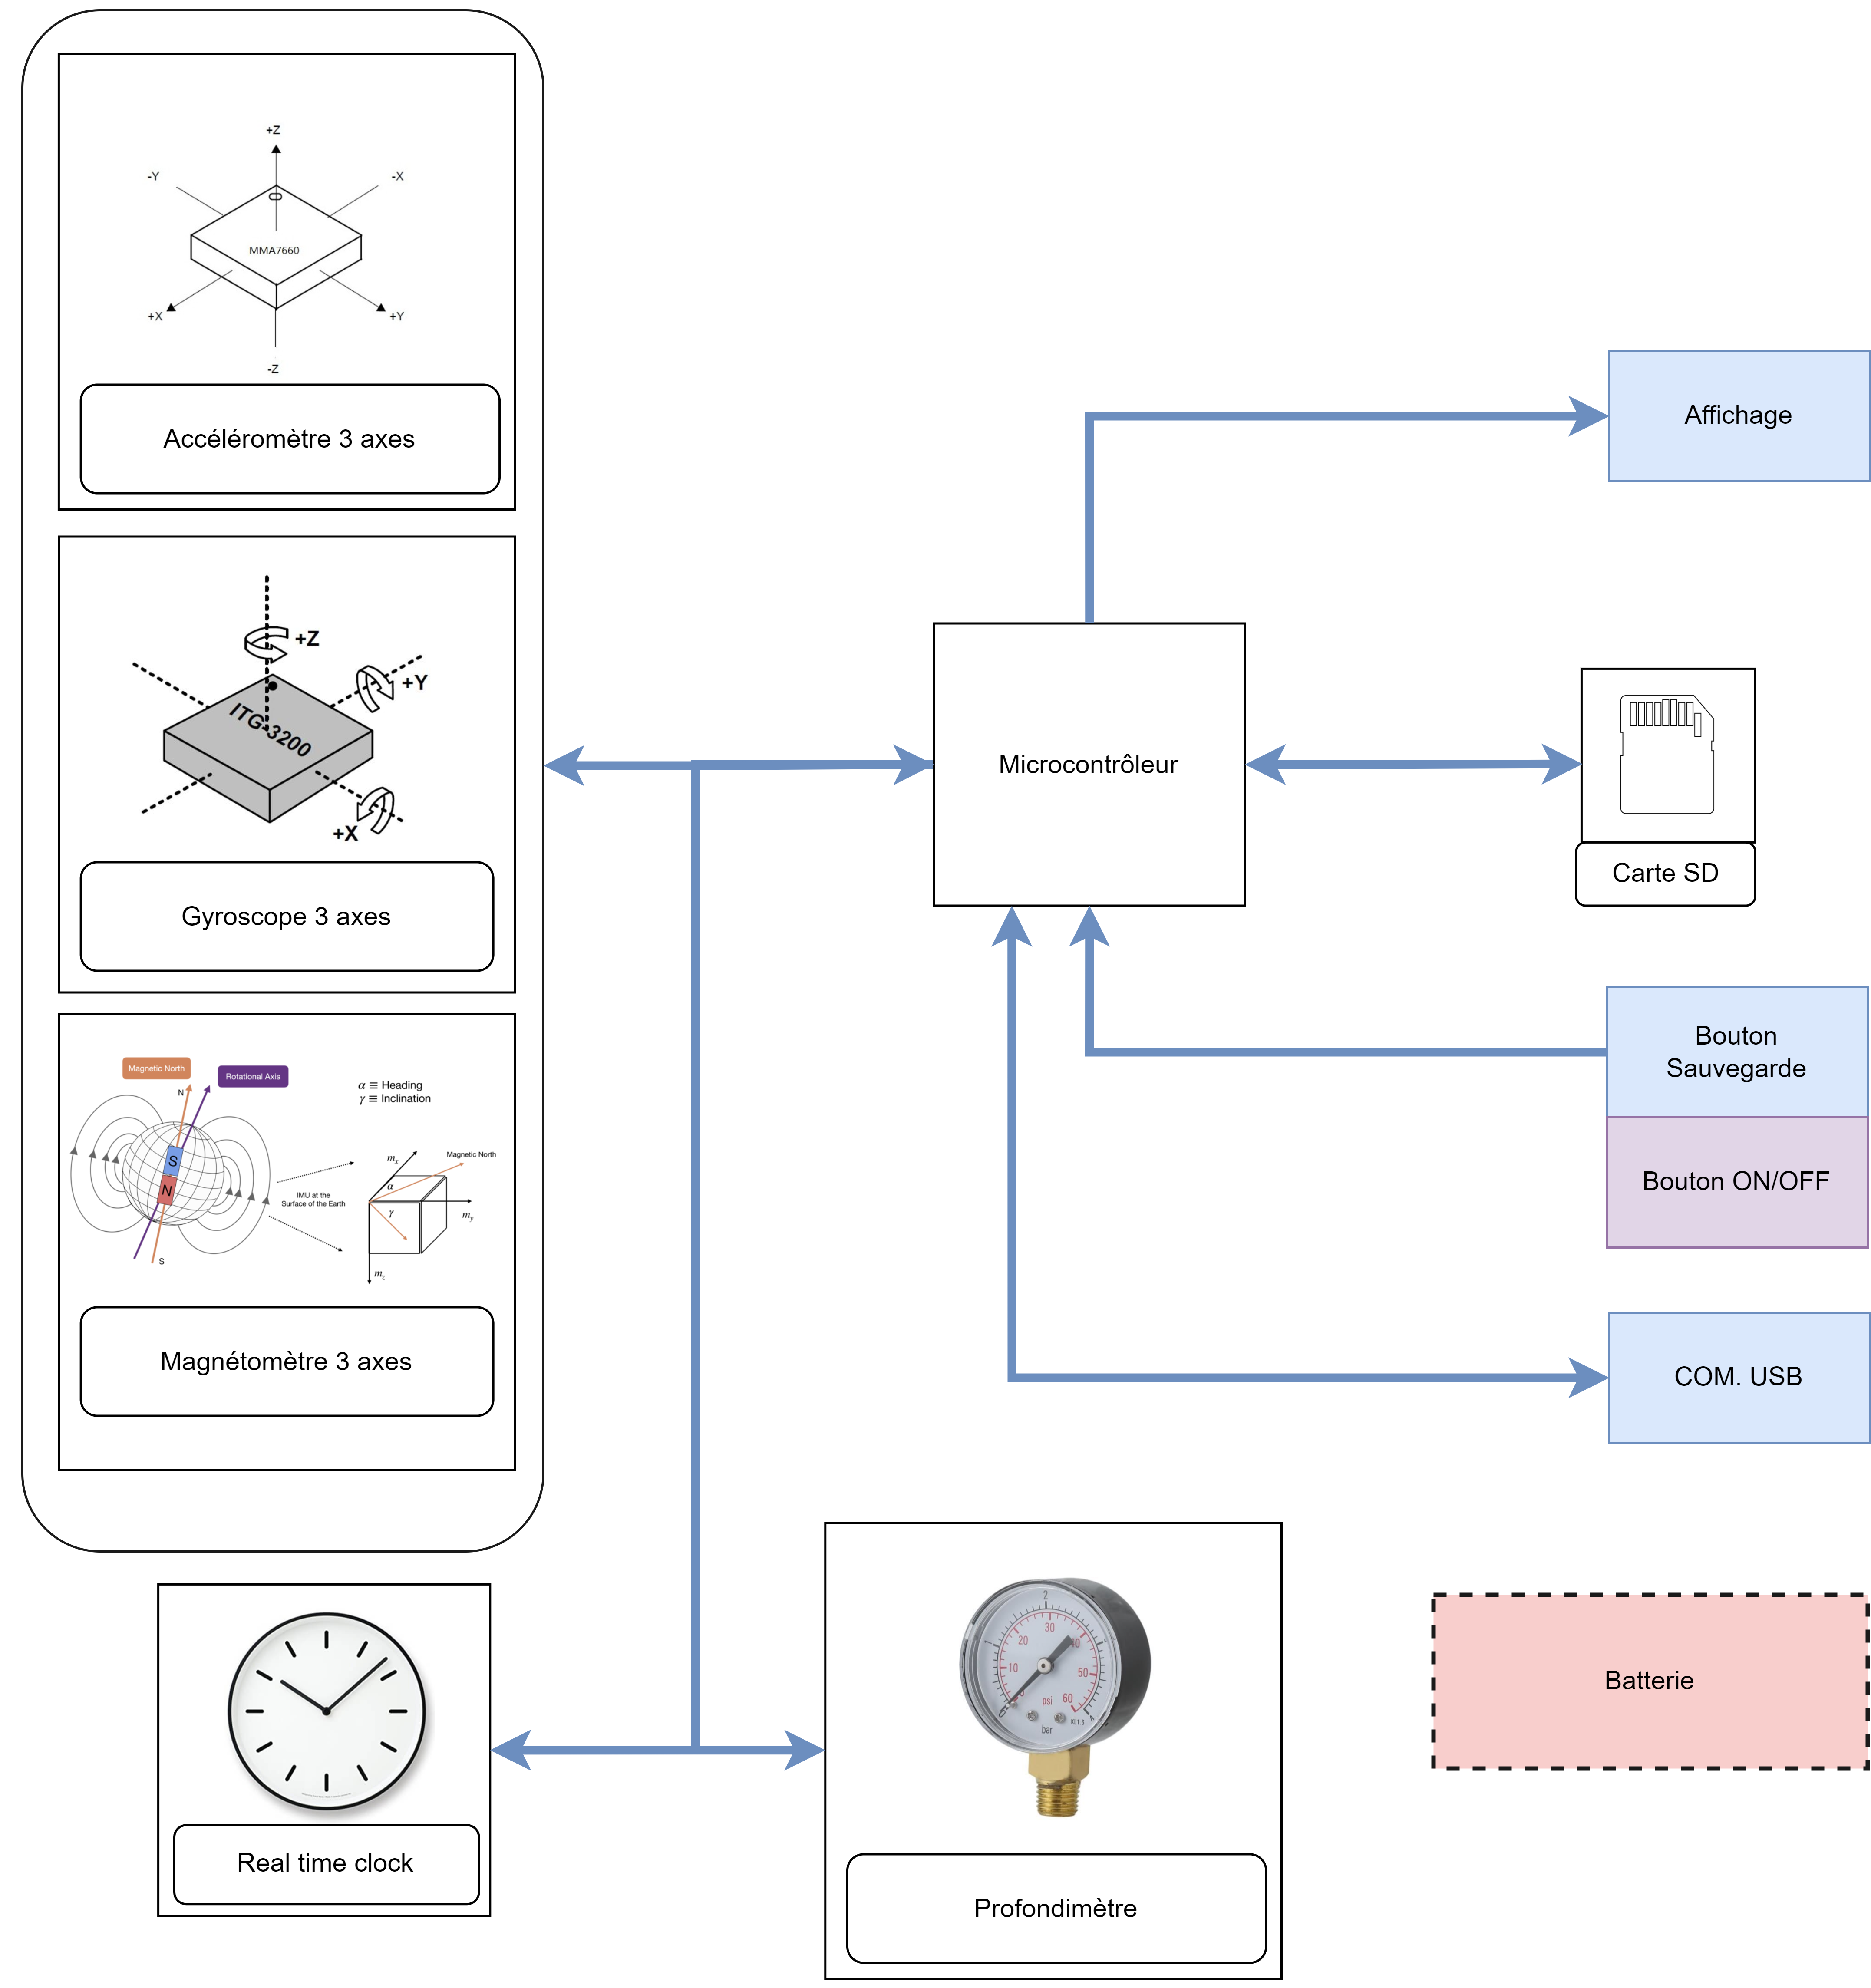
\includegraphics[width=.65\textwidth, center,]{../CDC/Figures/pre-etude.drawio.png}
    \caption{Schéma de principe}
    \source{Auteur}
\end{figure}
\clearpage

% ---- Description des blocs ----
\subsection{Description des blocs}
\begin{enumerate}
    \item \textbf{Carte SD :}\\
    Stockage des données de mesures chaque 100ms, cœur du projet.
    \item \textbf{Accéléromètre-gyroscope-magnétomètre :}\\
    Lecture des données individuelles brute ainsi que de fusion des capteurs, pour mesurer les déplacements sur 9 degrés de libertés.
    \item \textbf{Profondimètre :}\\
    Mesure la pression pour déduire la profondeur, afin de corroborer les autres mesures des capteurs.
    \item \textbf{Real time clock :}\\
    Permet de sauvegarder la temporalité du set de mesure dans la carte SD.
    \item \textbf{Affichage :}\\
    Affichage LED ou écran, pour affichage pas encore définis (ex. Profondeur, état batterie…)
    \item \textbf{Bouton sauvegarde :}\\
    Permet la mise en valeur d’un set de mesure. La forme de ce bouton n’est pas encore définie. Il sera peut-être fusionné avec le bouton ON/OFF.
    \item \textbf{Bouton ON/OFF :}\\
    Permet d’allumer ou d’éteindre le système.
    \item \textbf{Batterie :}\\
    Batterie du système, technologie à définir dans la pré-étude. 
    \item \textbf{COM. USB :}\\
    Permet de charger les batteries. Il faudra également prévoir dans cette version l’interface électronique pour la lecture de la carte SD directement par le port USB.
    \item \textbf{Microcontrôleur :}\\
    Lis et traite les valeurs des capteurs, sauvegarde dans la carte SD...
\end{enumerate}


\clearpage

% ---- JALONS ----
\subsection{Jalons principaux}
\begin{figure}[h!]
    \centering
    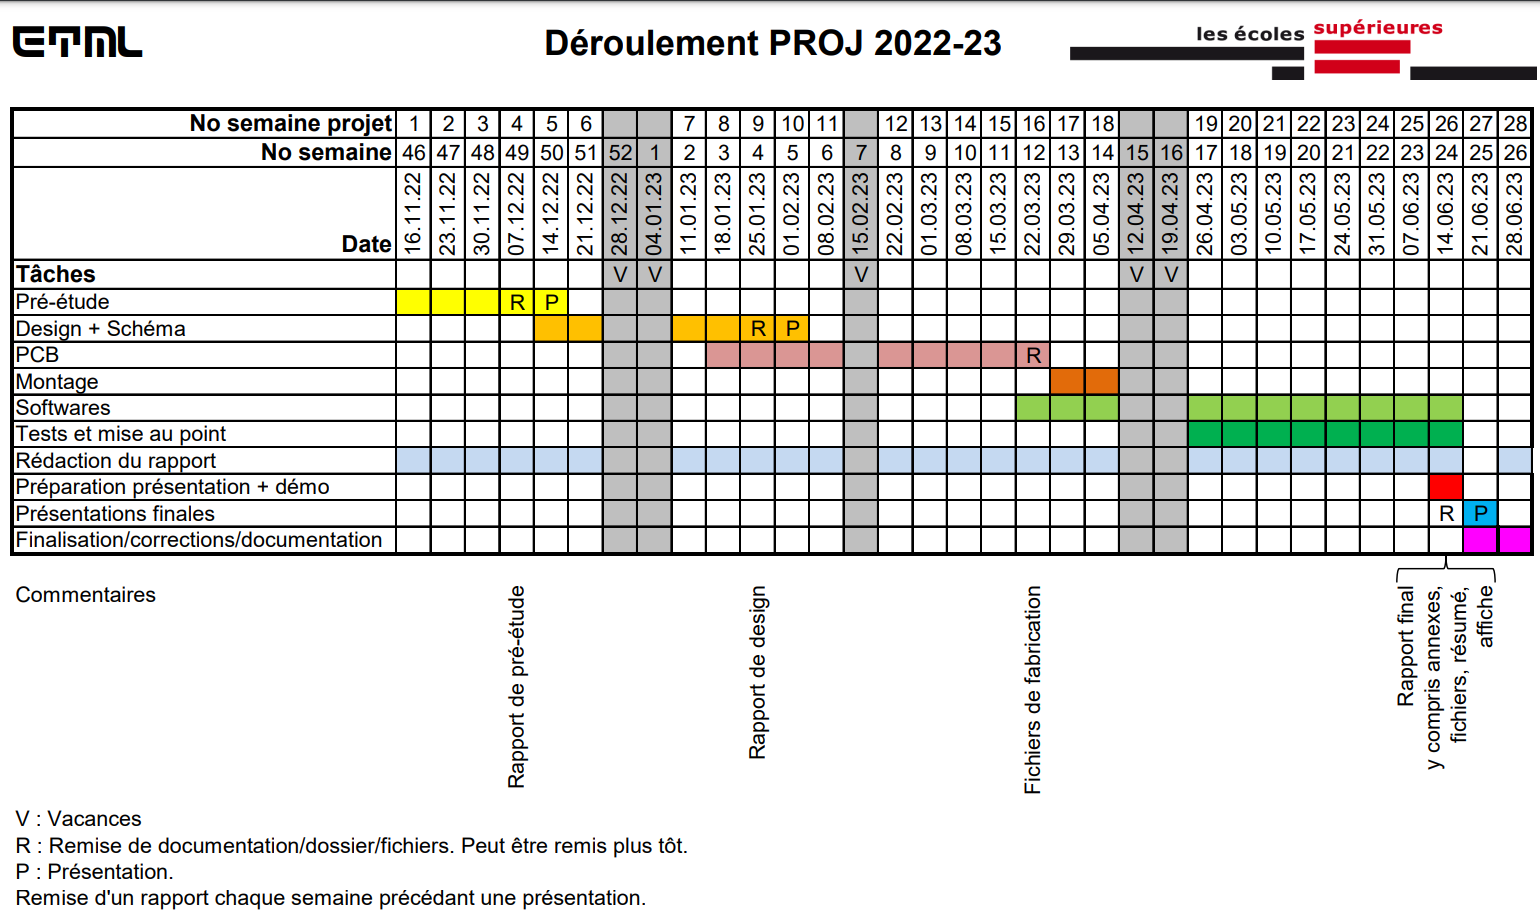
\includegraphics[width=.9\textwidth,center,]{../CDC/Figures/Tab-Jalons-PROJ.PNG}
    \caption{Jalons principaux}
    \label{fig:Jalons}
\end{figure}

\subsection{Livrable}
\begin{itemize}
    \item[•] Les fichiers sources de CAO électronique des PCB réalisés
    \item[•] Tout le nécessaire à fabriquer un exemplaire hardware de chaque :
    \item[•] fichiers de fabrication (GERBER) / liste de pièces avec références pour commande / implantation
    \item[•] Prototype fonctionnel
    \item[•] Modifications / dessins mécaniques, etc
    \item[•] Les fichiers sources de programmation microcontrôleur (.c  / .h)
    \item[•] Tout le nécessaire pour programmer les microcontrôleurs (logiciel ou fichier .hex)
    \item[•] Un calcul / estimation des coûts
    \item[•] Un rapport contenant les calculs - dimensionnement de composants - structogramme, etc.
\end{itemize}

\clearpage


% ------------------- PRE-ETUDE ---------------------- ----
% ------------------------- PRELIMINARY TASK -----------------------------
\section{Pré-étude}
L'objectif de cette pré-étude, est de se pencher sur le fonctionnement plus fondamental du système, faire des petits dimensionnements ainsi que de survoler différents aspects techniques liés au projet.
% ---------------- Subsection 1 ----------------
\subsection{Fonctionnement du système} \label{ssec:num01}
{
\subsubsection{Schéma bloc}

\begin{figure}[h]
    \centering
    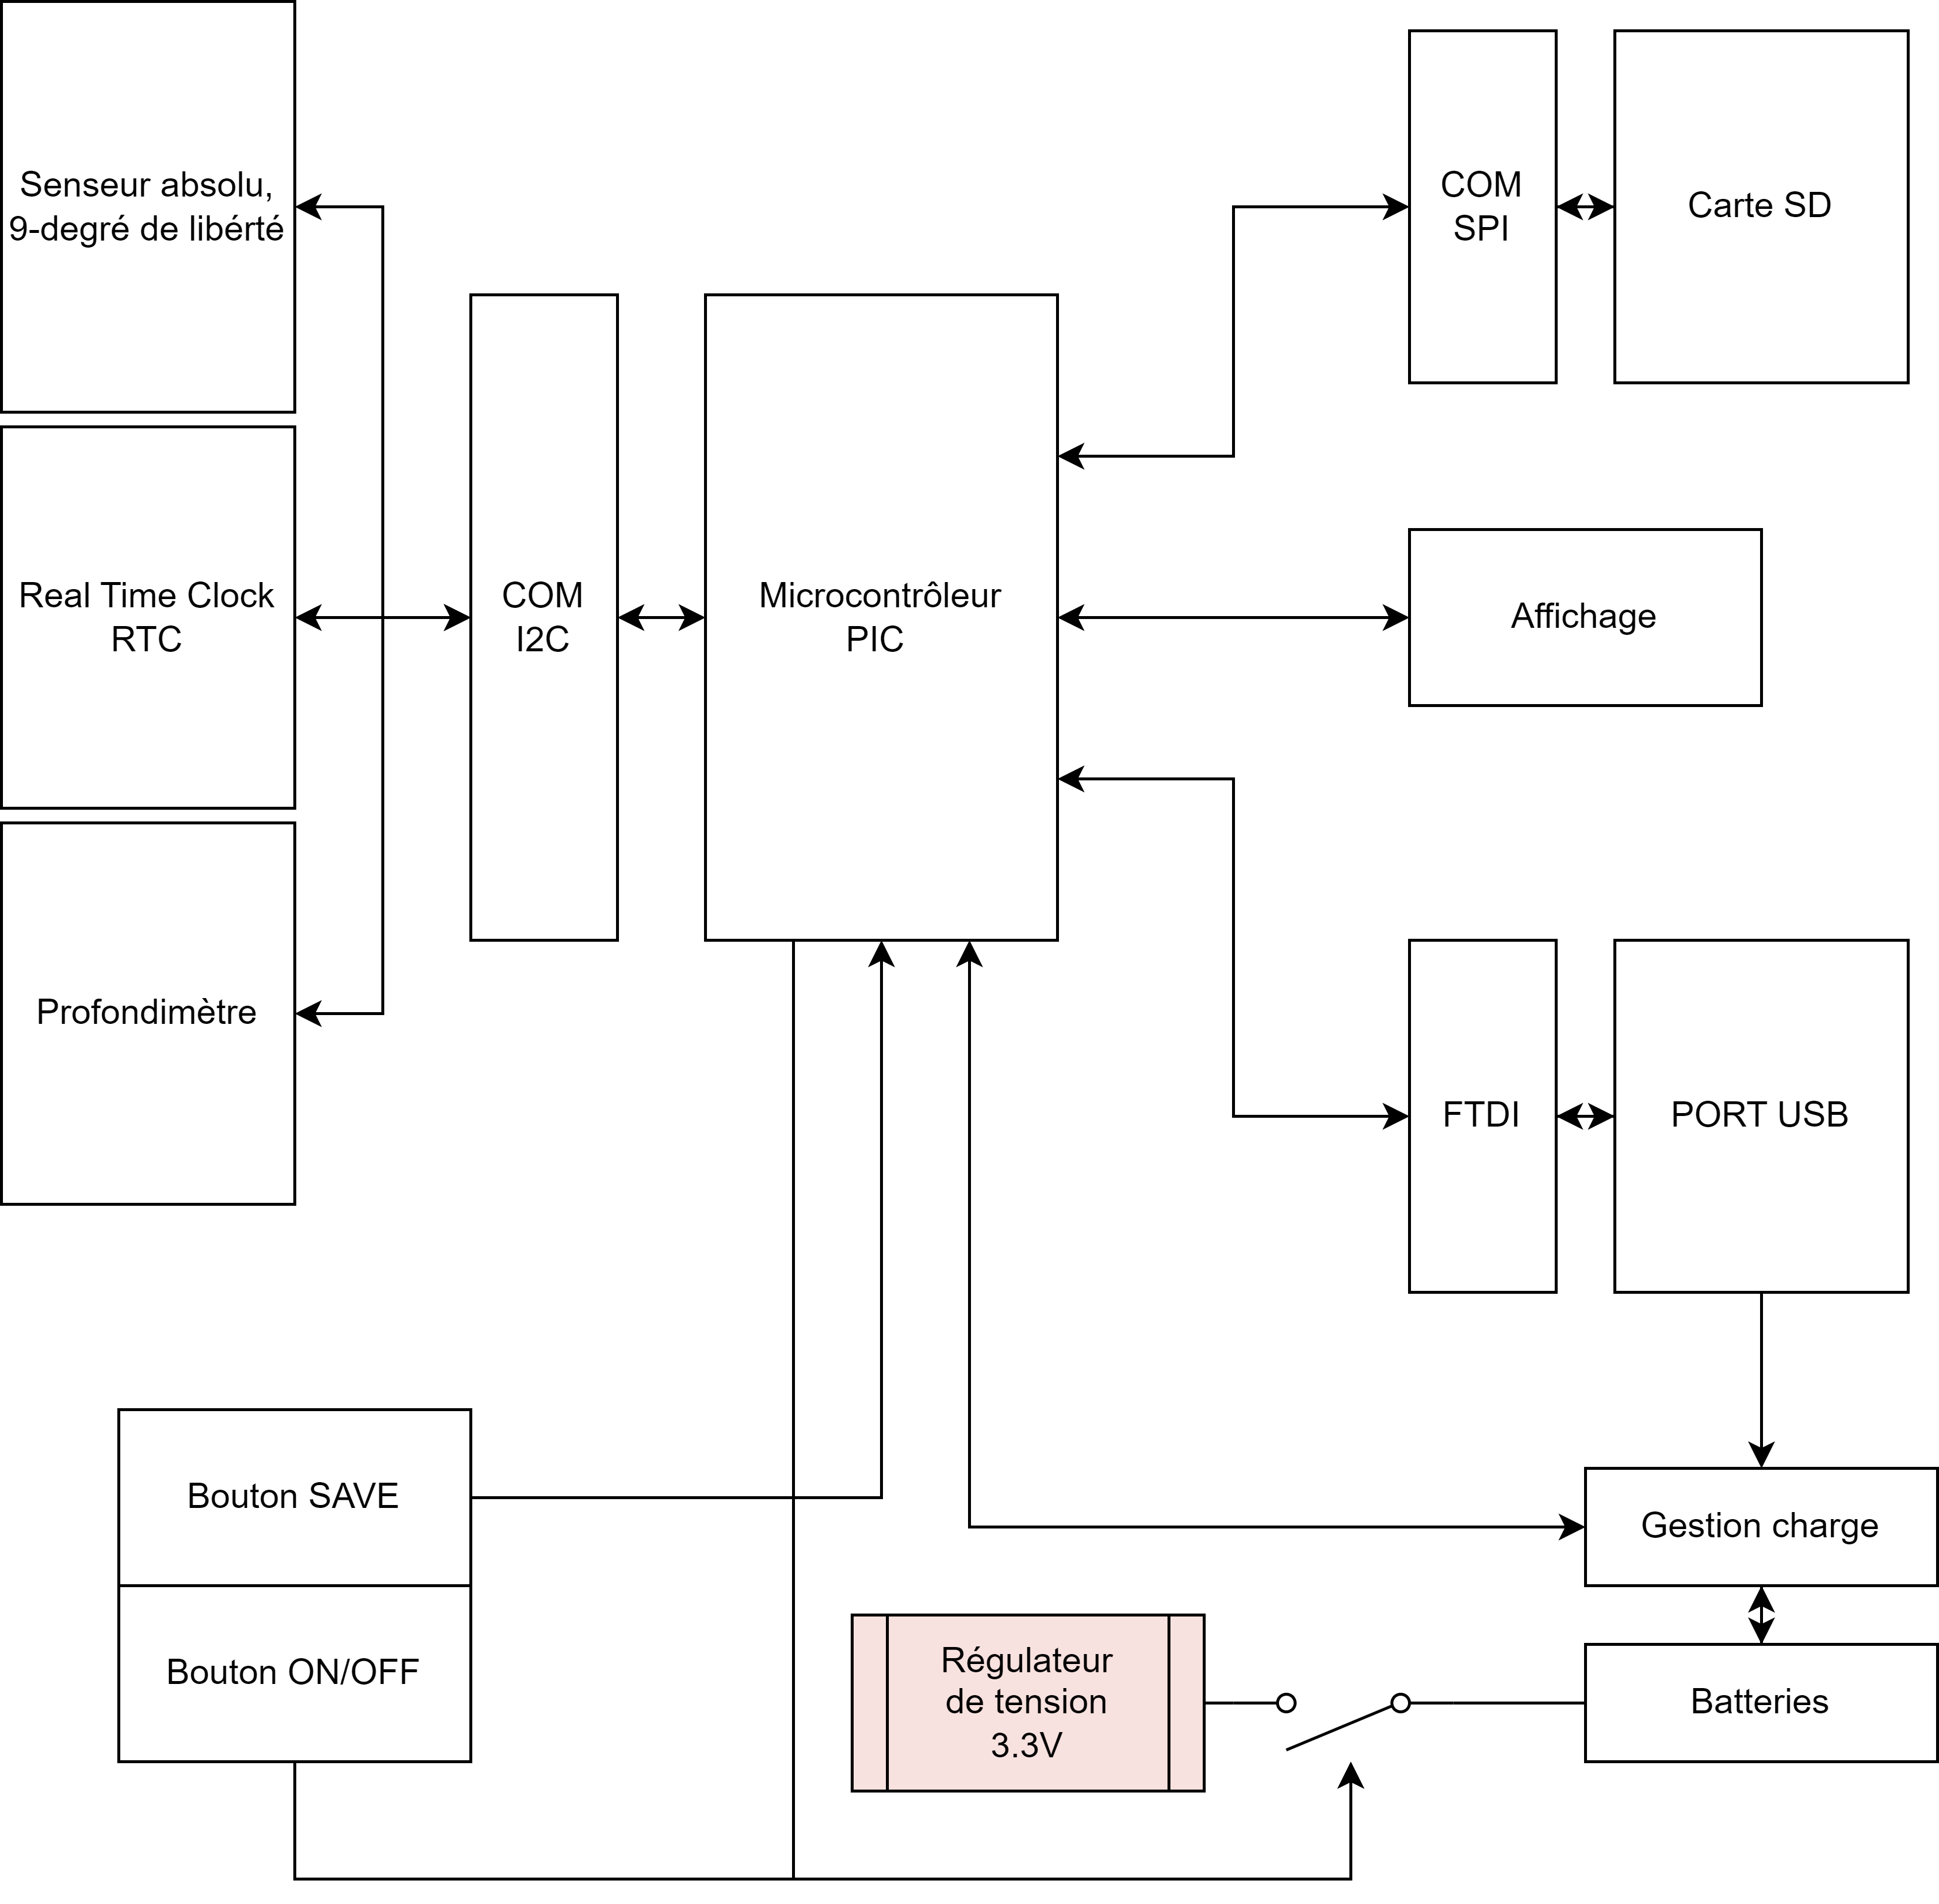
\includegraphics[width=.9\textwidth]{Figures/Schema-bloc-LocalisationSousMarin.drawio}
    \caption{Schéma bloc du module}
    \source{Auteur}
    \label{fig:SchemaBloc}
\end{figure}

\clearpage

\paragraph{Capteurs :} 
Les différents capteurs sont interfacés sur le même bus, et ont comme master le microcontrôleur en communication bidirectionnel, afin d'à la fois configurer les registres des périphériques et de lire leurs mesures.\\

\paragraph{Carte SD :}
La carte SD est interfacée en SPI et va contenir les données des différents capteurs ainsi que leurs éventuels flags d'importance (sauvegarde), sa taille sera dimensionnée ultérieurement.\\

\paragraph{Port USB \& charge :}
Un port USB est présent, afin charger les batteries par un IC de gestion de charge connecté directement au 5V. De plus le port USB est communiquant avec le microcontrôleur par un driver FTDI, afin d'éventuellement ajouter un système de lecture de la carte SD, directement par USB. Ceci dans cette version ou une ultérieure. Le port USB pourrait aussi servir a fixer la référence de la RTC. \\

\paragraph{Bouton multifonction :}
Sachant qu'un bouton étanche est déjà présent sur le module, l'exploiter en tant que bouton multifonction est une solution ergonomique pour ne pas mettre en péril l'étanchéité globale. Ce bouton ferait office de ON/OFF et de "sauvegarde" de point d'intérêt. Pour se faire, le bouton contrôlerait par un transistor de commutation l'alimentation du système, puis lors de l'allumage du microcontrôleur, le MCU prendrait la relève en maintenant le système allumé a sont tour, permettant ainsi de lire le bouton et de sur une pression longue déconnecter l'alimentation.\\

\paragraph{Affichage :}
L'affichage permettra de visualiser différentes données, dont les plus importantes tel que la pression ou le statut de la batterie. \\ La forme de l'affichage est encore a définir selon la mécanique du module, mais le plus élégant, serait l'utilisation d'un petit écran OLED.\\

\paragraph{Capteur de pression :}
Le capteur de pression devra avoir un contact direct avec l'eau, cela impliquera de la mécanique et de la gestion d'étanchéité. Une autre possibilité aurait été de mesurer optiquement la déformation du boîtier pour en déduire la pression, mais la complexité est trop importante.\\
}

\clearpage

% ----------------Subsection 2 ----------------
\subsection{Choix des composants importants} \label{ssec:num02}
{

\subsubsection{Senseur absolu}
{
    Pour le senseur absolu, il existe des IC permettant directement de faire la fusion des senseurs (\textbf{Accéléromètre, gyroscope, magnétomètre et thermomètre}), ce qui épargne toute une phase de calcul chronophage, en permettant directement de lire les \textbf{quaternion, angles de Euler, vecteurs de rotations, cap de direction etc...} directement sur le composant. Il existe différents IC dont deux ce sont montrés très intéressants, le \textbf{BNO85} et le \textbf{BNO55}, les deux étant PIN-Compatibles, j'ai décidé d'opter pour le \textbf{\underline{BNO055}}\footnote{\href{K:/ES/PROJETS/SLO/2221\_LocalisationSousMarine/doc/composants/9DOF-BNO055}{K:/ES/PROJETS/SLO/2221\_LocalisationSousMarine/doc/composants/9DOF-BNO055}}.
    
    \begin{figure}[h]
    \centering
    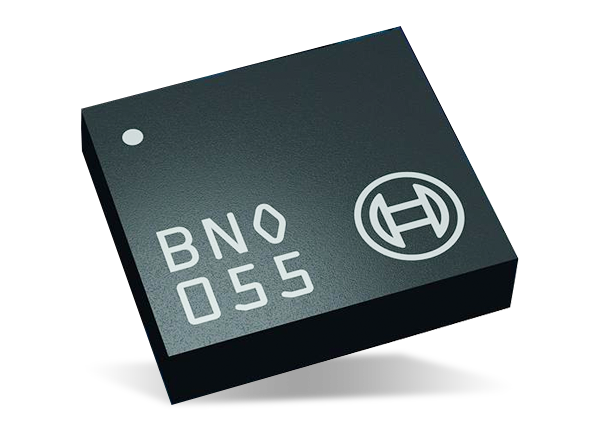
\includegraphics[width=.4\textwidth]{Figures/BNO055-Illustration}
    \caption{Schéma bloc du module}
    \source{\href{https://www.mouser.ch/new/bosch/bosch-bno55-sensor/}{https://www.mouser.ch/new/bosch/bosch-bno55-sensor/}}
    \label{fig:SchemaBloc}
    \end{figure}
    
    Sachant que la brazure de ce type de boîtier est compliquée et également dans un but de simplification du projet, j'ai décidé d'utiliser les cartes d'évaluation d'adafruit \textbf{N°: 4646} qui ont des connections bergs ainsi que tous les composants externes passifs déjà montés. \\
    
    \underline{Caractéristiques importantes :} \\
    
    \begin{tabular}{l l l l}
        Résolution gyroscope & : & 16 & [bits] \\
        Résolution accéléromètre & : & 14 & [bits] \\
        Résolution magnétomètre & : & $\sim$0.3 & [$\mu$T] \\
        $I_{DD}$ & : & 12.3 & [mA] \\
        Dérive de température & : & $\pm$ 0.03 & [\%/K] \\ 
        Dérive accéléromètre & : & 0.2 & [\%/V] \\
        Dérive gyroscope & : & <0.4 & [\%/V]
    \end{tabular} \\
    Nous allons par la suite voir sur la figure \ref{fig:BnoOut}, quelles données du BNO055 sont disponibles ainsi que leurs tailles mémoires.
    
    \begin{figure}[h] 
        \centering
        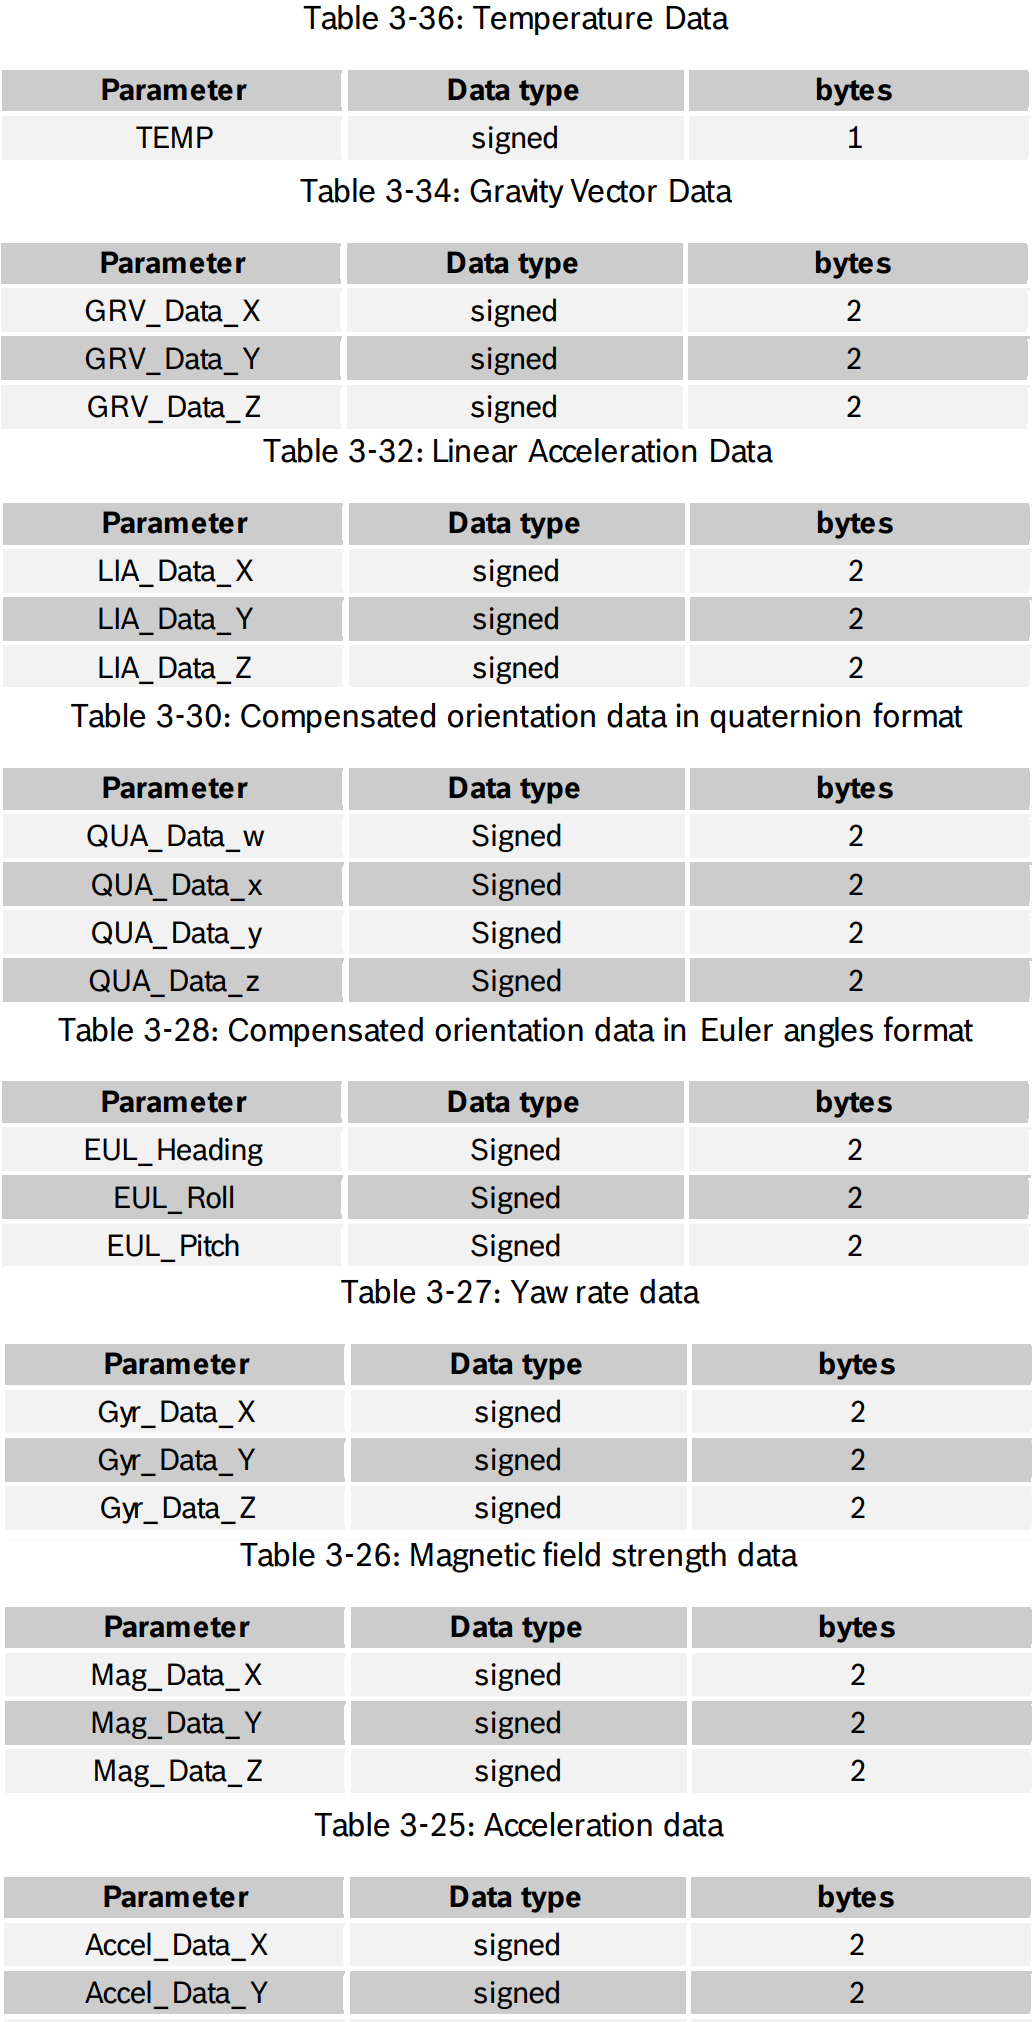
\includegraphics[width=.68\textwidth]{Figures/DATAS-BNO055}
        \caption{Donnée de sortie de l'IC (43 bytes)}
        \source{ \href{https://cdn-shop.adafruit.com/datasheets/BST\_BNO055\_DS000\_12.pdf}{https://cdn-shop.adafruit.com/datasheets/BST\_BNO055\_DS000\_12.pdf} }
        \label{fig:BnoOut}
    \end{figure}
}

\clearpage

\subsubsection{Capteur de pression}
{
Pour le capteur de pression, une modification mécanique du boîter sera très probablement nécessaire. J'ai pu trouver un capteur correspondant aux caractéristiques demandée du projet, celui-ci est plutôt générique et peut communiquer en I2C : \\
\textbf{PTE7300-14AN-1B016BN}

\begin{figure}[h] 
    \centering
    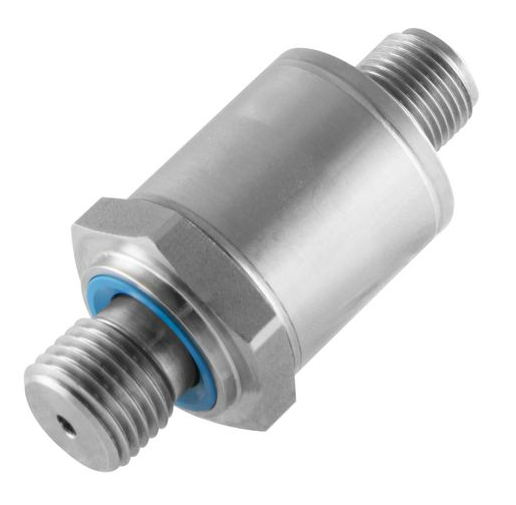
\includegraphics[width=.4\textwidth]{Figures/Capteur-pression}
    \caption{Illustration capteur de pression}
    \source{Distrelec, \href{https://www.distrelec.ch/fr/capteur-de-pression-hermetique-numerique-industriel-g1-16bar-module-sensata-pte7300-14an-1b016bn/p/30302457}{PTE7300-14AN-1B016BN}}
    \label{fig:CaptPress}
\end{figure}

L'avantage avec le capteur ci-dessus est le système hermétique pour le trou, un autre capteur peut être utilisé lors de l'étude, néanmoins la modification mécanique étant probablement inévitable, le système de vissage de la figure \ref{fig:CaptPress} est intéréssant.

}

\subsubsection{Affichage}
{
    Pour l'affichage, je vais essayer d'opter pour un petit afficheur OLED, en gardant la possibilité en cas de de complication lors de l'étude, l'utilisation de simples LEDS d'indications.
    \\
    Il existe plusieurs affichages OLED rond petits formats, sur lesquels je me pencherais plus en détail lors de l'étude.
    


}

\newpage
\subsubsection{Carte SD} \label{sssec:CarteSD}
{
    \paragraph{Taille mémoire : }
    Afin de dimensionner la taille de stockage de la carte SD, il faut utiliser les différentes caractéristiques du projet. Normalement la taille de la carte SD n'est clairement pas un problème, sachant que seulement du texte est enregistré et que les tailles mémoires disponibles peuvent être très élevées. Néanmoins il est intéressant de faire le dimensionnement pour connaître le minimum, et pour éventuellement adapter le projet avec d'autres systèmes de mémorisation.  \\
    Où : \vspace{+14pt} \\
    \begin{tabular}{l l ll|l}
       $ T_{rec} $ & = &  $7200'000$ & $[ms]$ & Temps a enregistrer \\
       $ T_{ech}$ & = & $100$  & $[ms]$ & Temps d'un échantillon \\
       $ S_{mes} $ & = & $150$ & $[bytes]$ & Taille de toutes les données de mesures  \\
       $ S_{timestamp} $ & = & $\sim$3 & $[bytes]$ & Taille de l'information de temporalité  \\
       $ S_{flag} $ & = & $ 1 $ & $[bytes]$ & Taille de l'indication d'importance 
    \end{tabular}
    \vspace{+14pt}
    \\
   \paragraph{ Nombre de mesure a effectuer :}
    \begin{equation} \label{equ:NbMes}
        Nb_{mesures} = \frac{T_{rec}}{T_{ech}}
    \end{equation} 
    D'après (\ref{equ:NbMes}), nous avons un nombre de mesure de 72'000.  \vspace{+8pt} \\
    
   \paragraph{Taille minimum :}
    \begin{equation} \label{equ:TailleMin}
        Taille_{min} = Nb_{mesures} * (S_{mes}+S_{timestamp}+S_{flag}) 
    \end{equation}
    D'après (\ref{equ:TailleMin}), la taille mémoire minimum doit être de \textbf{$\sim$11MB}. \vspace{+8pt} \\ 
    Nous pouvons donc constater que pour une utilisation standard de 2h, la mémoire occupée est très faible, d'où l'intérêt de sauvegarder dans la carte SD la date, afin de pouvoir faire plusieurs "expéditions" en "une fois", sans avoir à vider la carte.
}

\newpage
\subsubsection{Real Time Clock}
{
    L'objectif de la RTC, est de donner l'information de la temporalité de la mesure (timestamp), afin de lors du traitement des donnée avoir accès à ce paramètre. \\
    Sachant que l'échantillonnage des mesures est de 100ms, la RTC devrait permettre cette résolution. Néanmoins une autre information importante, comme mentionnée lors de la section \ref{sssec:CarteSD}, est la date de la mesure, afin de permettre plusieurs expéditions par utilisation de la carte. \vspace{+8pt} \\
    J'ai donc décidé d'utiliser une RTC pour l'heure grossière de départ (Année, date, heure, minute, seconde) et les compteur du MCU pour faire le delta entre chacune des mesures en ms. \\

    La RTC devra pouvoir tenir le minimum de 2 heure d'utilisation, à cette fin, la batterie LI-ION déjà présente sera suffisante. \\ 
    La RTC devra avoir une faible consommation, le calendrier ainsi qu'une bonne précision. A cette fin, la RTC \textbf{S-35390A-T8T1G} est assez générique et possède une bonne documentation.
     
    
}

\subsubsection{Microcontrôleur}
{
    Le microcontrôleur devra avoir un nombre suffisant de communications, sachant que beaucoup sont présentes dans le projet (\textbf{I2C, SPI, UART...}), ce qui signifie un nombre de pattes élevées. 
    
    
    Des calculs peuvent aussi être nécessaire, si il s'avère qu'il faille faire une traitement des données préliminaire, il faudrait donc opter pour un MCU 32bits si possible.


    La famille PIC est celle standardisée par l'école supérieure, c'est donc pour cette famille-ci que je vais opter.
    \vspace{+12pt} \\

    \begin{figure}[h] 
        \centering
        
\includegraphics[width=.4\textwidth]{Figures/PIC32MX795F512L-V7X-Regular}
        \caption{Illustration du modèle MCU du kit ETML-ES}
        \source{\href{https://www.microchip.com/en-us/product/PIC32MX795F512L}{https://www.microchip.com/en-us/product/PIC32MX795F512L}}
        \label{fig:MCU}
    \end{figure}
    
}

\clearpage

\subsubsection{Batterie, charge et régulation}
{

Pour la technologie de batterie, en utilisation sous-marine, j'ai trouvé ce tableau de comparaison :

\begin{figure}[h]
    \centering
    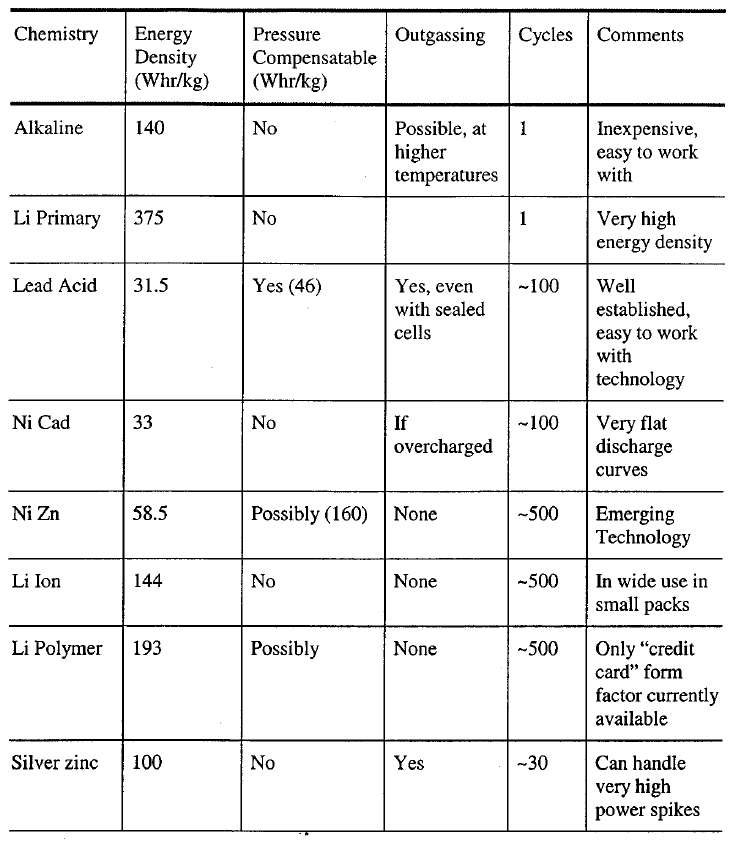
\includegraphics[width=.56\textwidth]{Figures/PowerSystemsComparison}
    \caption{Comparaison des technologies de batteries}
    \source{Power Systems for Autonomous Underwater Vehicles\cite{bradley_power_2001}}
    \label{fig:BatteriesComparaisons}
\end{figure}

Pour des raisons de praticité et étant-donné la documentation plus importante, j'ai décidé d'utiliser la technologie \textbf{LI-ION} : \\

\begin{table}[h]
	\centering
	\begin{tabular}{l|l}
		Avantages &  Inconvénient\\
		\hline
		Haute densité d'énergie & Risque d'éclatement \\
		Poids léger & Risque d'enflammement avec l'eau \\ 
		Haute durée de vie & Sensible a la température \\
		Charge rapide & Décharge complète altérante \\
	\end{tabular}
	\caption{Tableau avantages/inconvénient LI-ION)}
\end{table}

\vspace{+8pt}

Malgré les risque dûs au contact de l'eau (\textbf{Enflammement, éclatement...}) la technologie LI-ION est souvent utilisée pour les application sous-marines dû a ses différents avantages, c'est pour cela que j'opterais pour cette technologie. 

}

}

\newpage
\subsection{Estimation des coûts} \label{ssec:EstPrix}
{
    Ici je vais me baser sur les composants que j'ai pu trouver et estimer le coût moyen de ceux-ci, c'est a titre purement indicatif, (les prix sont généralement estimés a la hausse).
    \vspace{+12pt}
    
    \begin{center}
        \begin{tabular}{l|l}
            Composant & Estimation \\
            \hline
            Profondimètre & 70.- \\
            Centrale inertielle & 35.- \\
            RTC & 5.- \\
            Microcontrôleur & 5.- \\
            Carte SD & 20.- \\
            Affichage OLED & 45.- \\
            FTDI & 4.- \\
            Batterie LI-ION & 20.- \\
            IC chargeur & 4.- \\
            Traco-power 3.3V & 10.- \\
            PCB & 40.- \\
            \hline
            \hline
            Total & 258.-
        \end{tabular} 
    \end{center}
	

    L'estimation des prix étant plutôt élevée, des économies peuvent être très facilement réalisées, en changeant l'affichage OLED pour des LEDS ou en modifiant le PCB (Le simplifier ou changer de fournisseur (eurocircuit)).

}

\subsection{Synthèse développement} \label{ssec:PreeConc}
{

J'ai pu lors de cette pré-étude, établir le fonctionnement global du système, choisir certaines technologies et composants importants, ainsi que pu procéder a certains dimensionnements utiles quant au futur développement. 
Par la suite, je vais affiner les différents éléments abordés lors de la pré-étude, effectuer le développement plus détaillé de chacun des blocs et réaliser la schématique du projet.
Lors de la pré-étude, je n'ai pas eu accès au boîtier mécanique du projet, ce qui a restreint mon champs d'action lors de certains dimensionnement, tandis que pendant l'étude j'aurais accès a celui-ci, ce qui risque d'impacter/modifier certains aspect fixés lors des section antérieures.
Je suis très intéressé par le projet et me réjouis grandement de poursuivre son développement.

}

\clearpage


% ---------- DÉVELOPPEMENT SCHÉMATIQUE --------------------
% ------------------------- MAIN TASK ---------------------------------
\section{Développement schématique}

\subsection{Choix des composants} \label{ssec:num32}
{
	\subsubsection{Microcontrôleur}
	Lors de la recherche de composants, j'ai décidé d'utiliser l'un des PIC32 standards de l'ES :
	\textbf{PIC32MX130F064D-I/PT}.
		
	\begin{figure}[h]
		\centering
		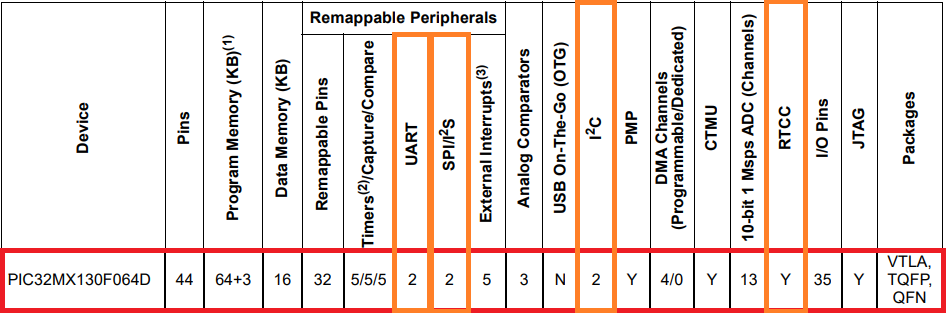
\includegraphics[width=1\linewidth]{Figures/Dev-SCH/PIC32-choisi}
		\caption{Périphériques disponibles du PIC}
		\label{fig:pic32-choisi}
		\source{PIC32MM0256GPM064 family datasheet}
	\end{figure}
	
	Nous pouvons constater sur la figure \ref{fig:pic32-choisi} que les critères minimaux de mon projet sont respectés :
	
	\begin{center}
		\fbox{\textit{1 - I2C}} \fbox{\textit{1 - SPI}} \fbox{\textit{1 - UART}} \fbox{\textit{1 - RTCC}}
	\end{center}
}

\clearpage
\subsection{Dimensionnements} \label{ssec:num31}
{
	\subsubsection{Vue d'ensemble schématique} \label{sssec:SchemaBloc} \vspace{-6mm}
	{
		\begin{figure}[th]
			\centering
			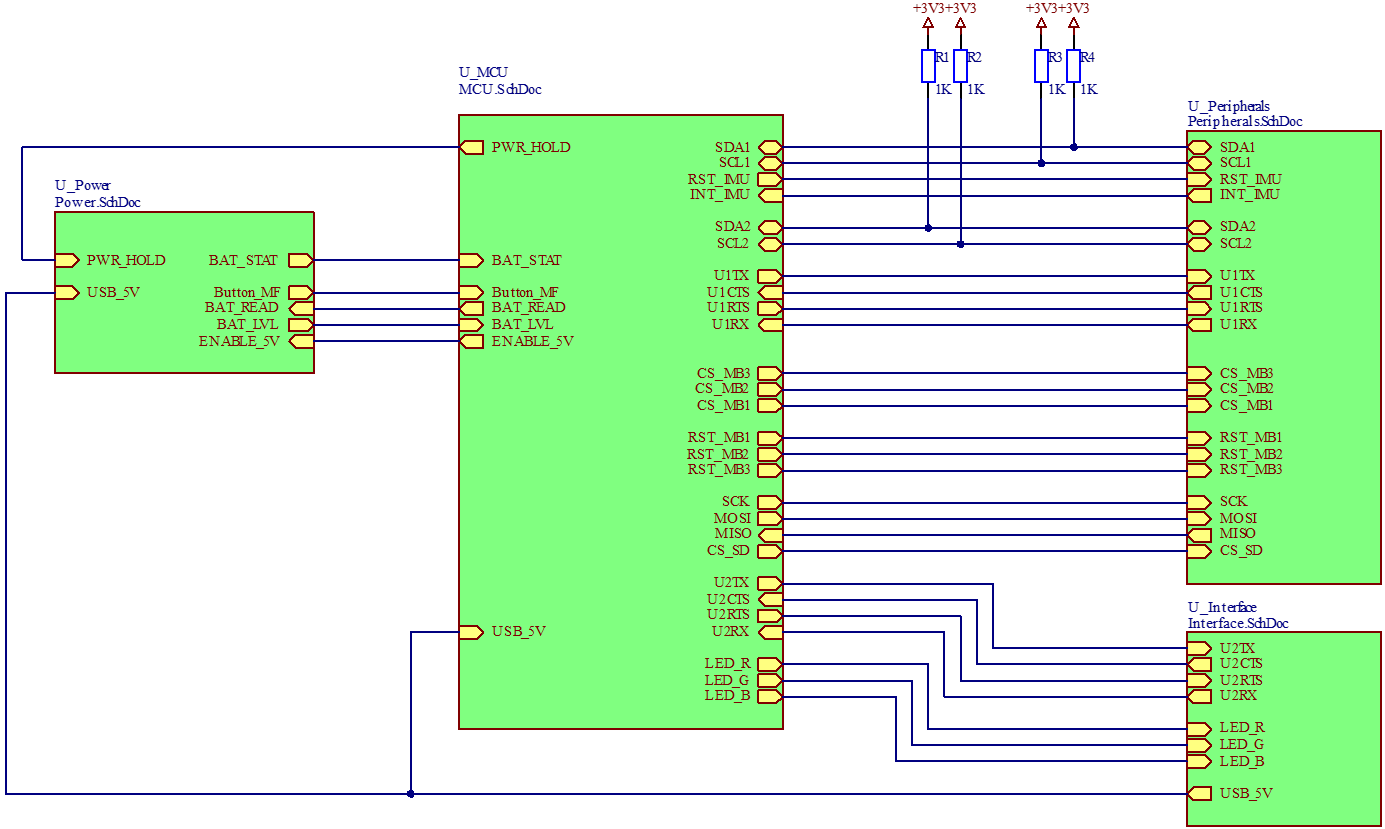
\includegraphics[width=1.1\linewidth]{Figures/Dev-SCH/schemaBloc}
			\caption{Schéma bloc de la schématique}
			\source{Auteur}
			\label{fig:schemablocSCH}
		\end{figure} \vspace{-5mm}
		Nous pouvons constater sur la figure \ref{fig:schemablocSCH} la structure des différents blocs du schéma : 
		
		\begin{tabularx}{18cm}{|X|X|}
			\hline
			Bloc & Description \\
			\hline
			\hline
			Power & Contient les différents régulateurs du système, ainsi que la gestion de charge de la batterie. \\
			\hline
			MCU & Contient l'intelligence du système, avec le microcontrôleur ainsi que tous ses composants passifs associés. \\
			\hline
			Peripherals & Périphériques du système : Carte-SD, Centrale inertielle, Capteur de pression, Slots MikroE. \\ 
			\hline
			Interface & Connecteur USB avec convertisseur serial (FTDI) et tous les composants passifs de sécurité. Interface LED RGB pour le statut. \\
			\hline
		\end{tabularx}
	}


	\clearpage
	\subsubsection{Autonomie du système} \label{sssec:SysAutonomie}
	{
		Afin de proportionner la batterie du circuit, il a fallut dimensionner les différentes consommations des composants, ceci par le biais de leurs documentations :
		
		\begin{center}
			\fbox{\textit{MCU - 30mA}} \fbox{\textit{BNO055 - 12.3mA}} \fbox{\textit{Capt. Pression - 4mA}} \fbox{\textit{\textcolor{red}{Carte-SD - 100mA}}} \fbox{\textit{MikroE - ??mA}} \fbox{\textit{Régulateurs - 40uA}} \fbox{\textit{LED RGB - 25mA}} 
		\end{center}
		
		Nous pouvons constater que la plus grande consommation vient de la carte micro-SD, qui au maximum peut induire 100mA. \footnote{Selon datasheet SanDisk : https://images-na.ssl-images-amazon.com/images/I/91tTtUMDM3L.pdf}
		
		
		Afin d'obtenir une autonomie d'au moins 2h (selon CDC), il faudrait une capacité de :
		
		\begin{equation}
			Capacite = Consommation_{tot} * Temps
		\end{equation}
		
		Ce qui nous fait une capacité de $\sim$342.68mAh, valeur facilement atteignable par les batteries li-ion du marché. Étant-donné que différents projets utilisaient des batteries 3400mAh, dans un objectif de conformité et de simplification des commandes, j'ai choisis cette même valeur.
		Ce qui signifie une autonomie de $\sim$20 heures, sans compter les différents mécanismes d'économie d'énergie.
		
		C'est un temps largement suffisant pour la durée de plusieurs expéditions, néanmoins la RTCC du microcontrôleur requiert d'être alimentée en permanence, j'ai donc décidé de déterminer un fonctionnement, où lorsque l'on charge la batterie la date se mettrait à jour et le mode "éteint" serait juste un mode de veille qui attendrait un niveau positif sur le switch avant de commencer le logging avec un timsetamp principale contenant la date, puis, seulement des deltas entre les mesures. Un diagramme des états est présents à la figure \ref{fig:etatsdiagramme}.
		
		\clearpage
		\begin{figure}[th]
			\centering
			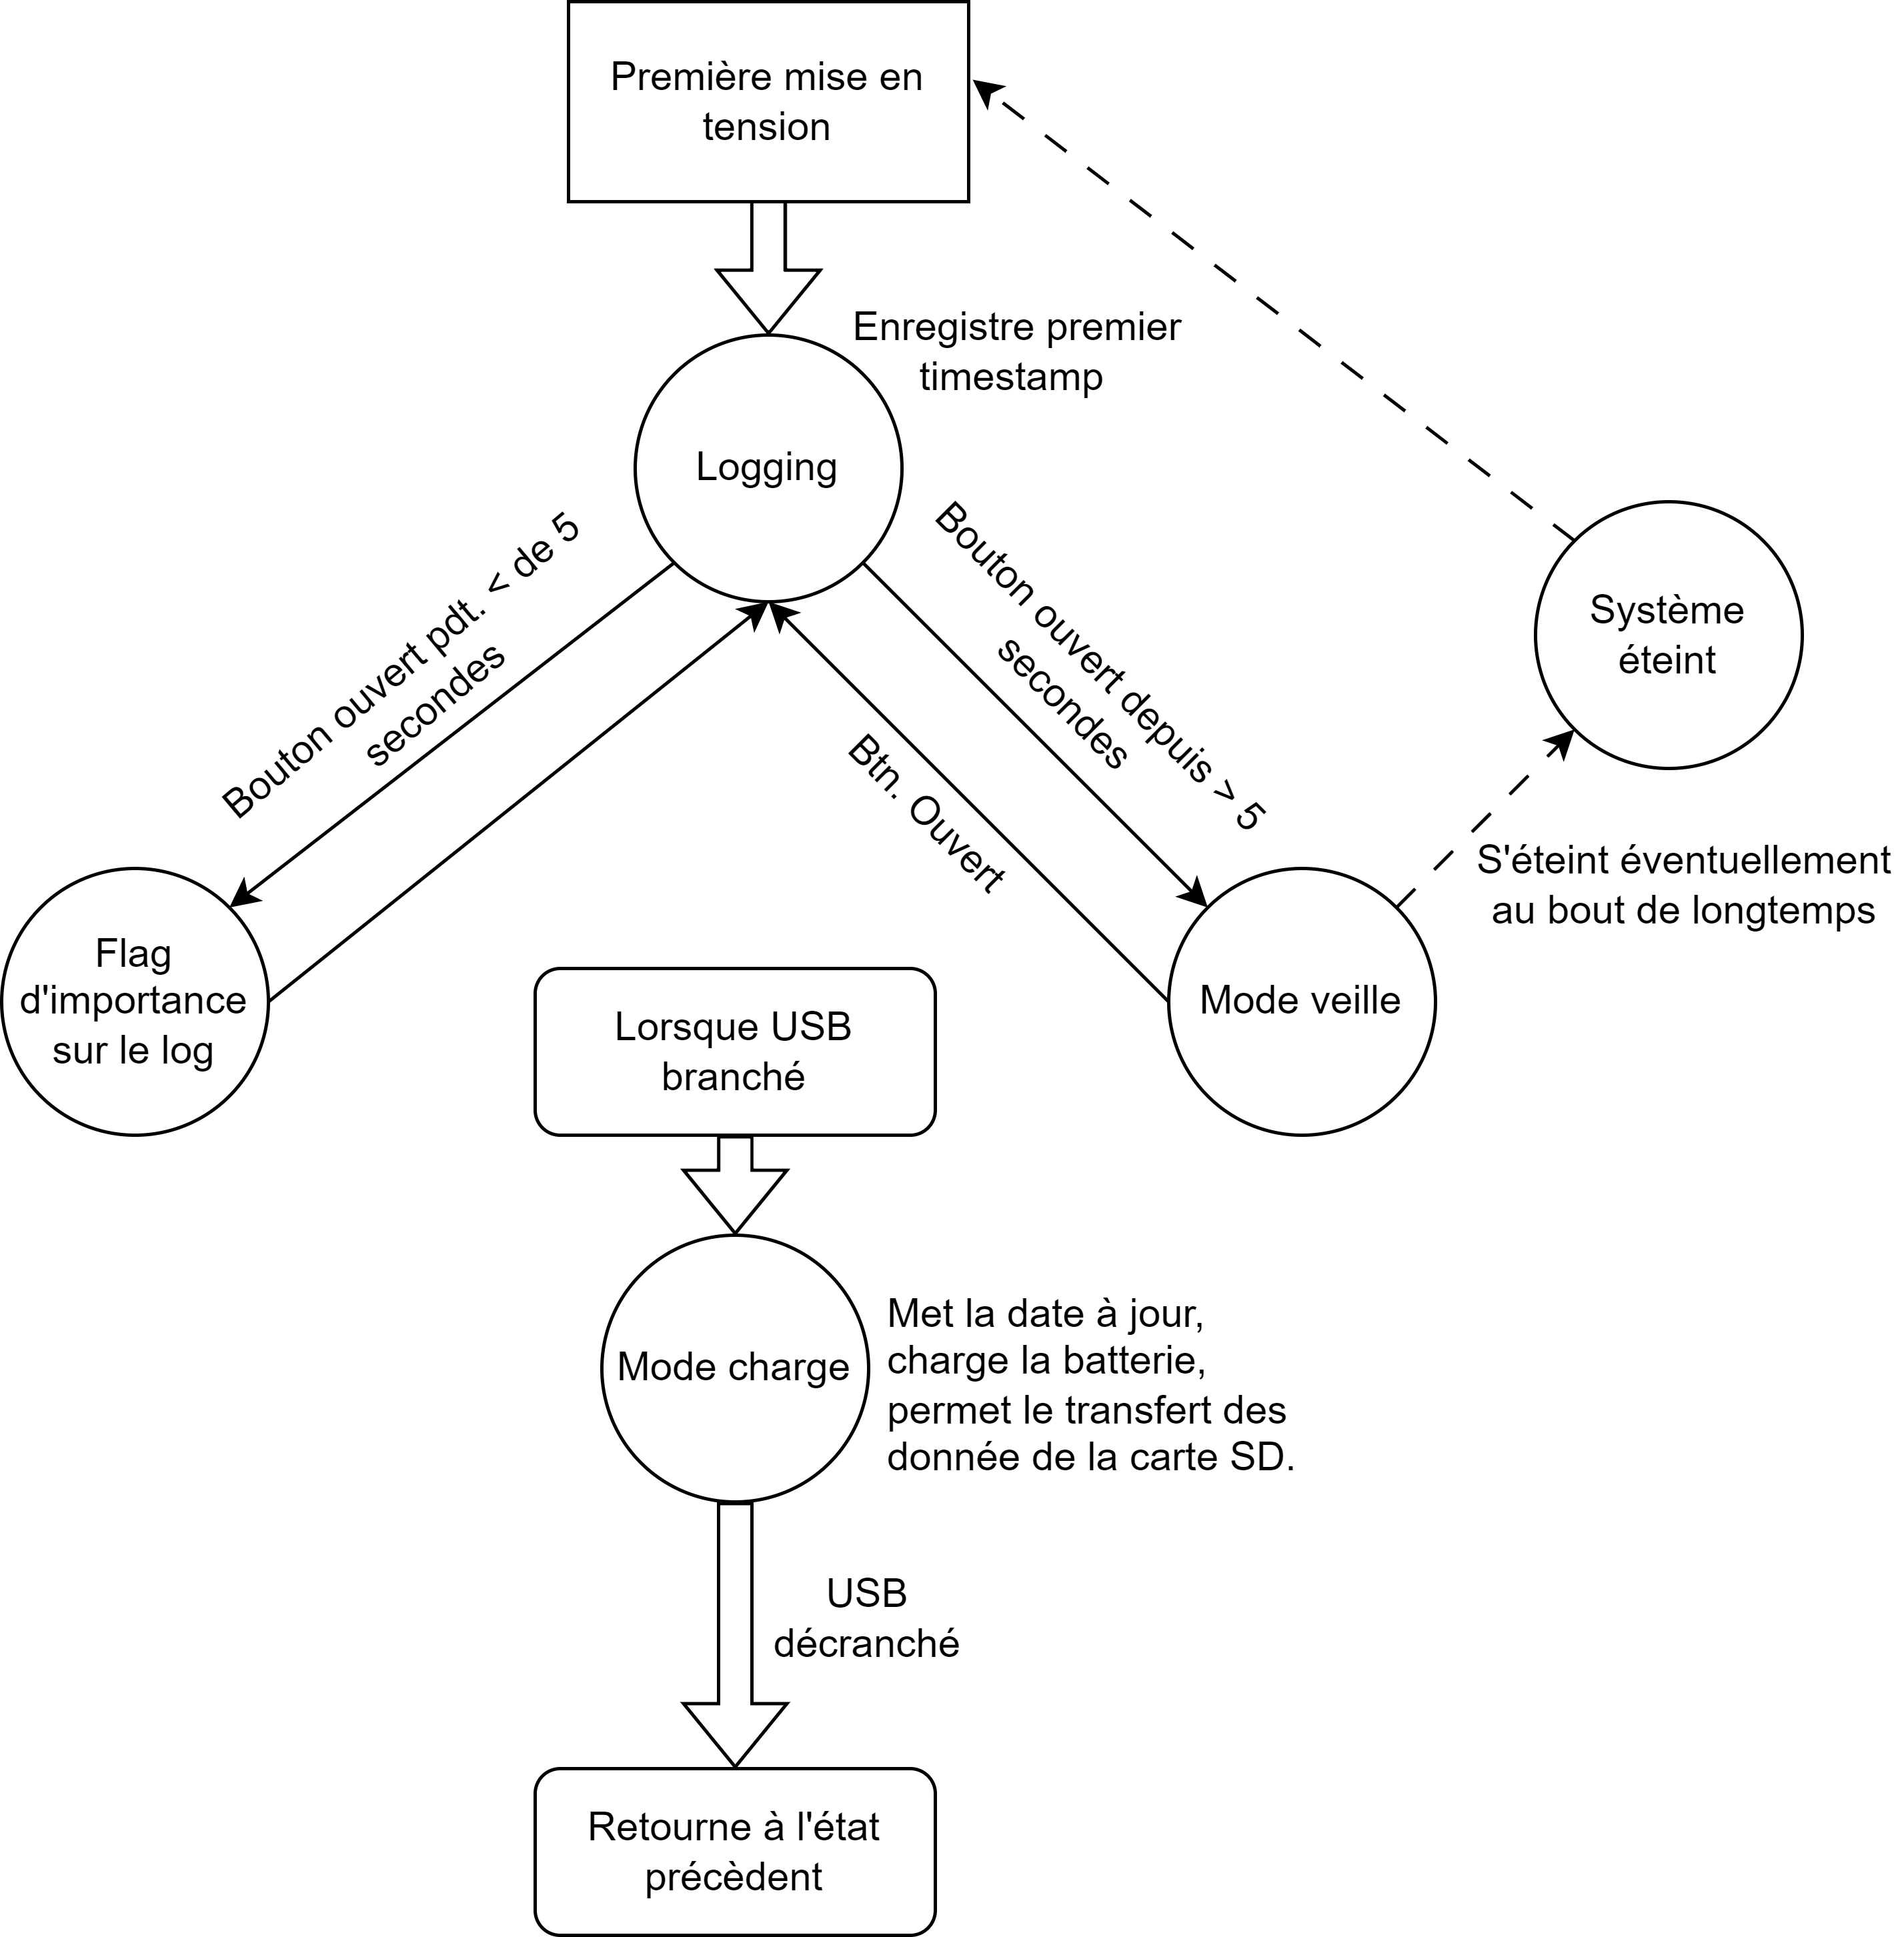
\includegraphics[width=1.1\linewidth]{Figures/Dev-SCH/Etats_diagramme}
			\caption{Diagramme des états du système}
			\label{fig:etatsdiagramme}
			\source{Auteur}
		\end{figure}
		
	}

	\clearpage
	\subsubsection{LED Interface} \label{sssec:DimLedRGB}
	{
		Afin d'informer l'utilisateur de ce qu'il se passe dans le système, j'ai décidé d'implémenter en tant qu'interface, une led RGB. Celle-ci sera un minimum puissante, afin de pouvoir être lisible lors de l'utilisation sous-marine du module.
		
		La consommation de la led RGB étant relativement importante, des mécanismes d'économie d'énergie seront mis en place dans le développement firmware. \vspace{+3mm}
		
		\textbf{Diagramme d'interface :}
		
		\begin{figure}[h]
			\centering
			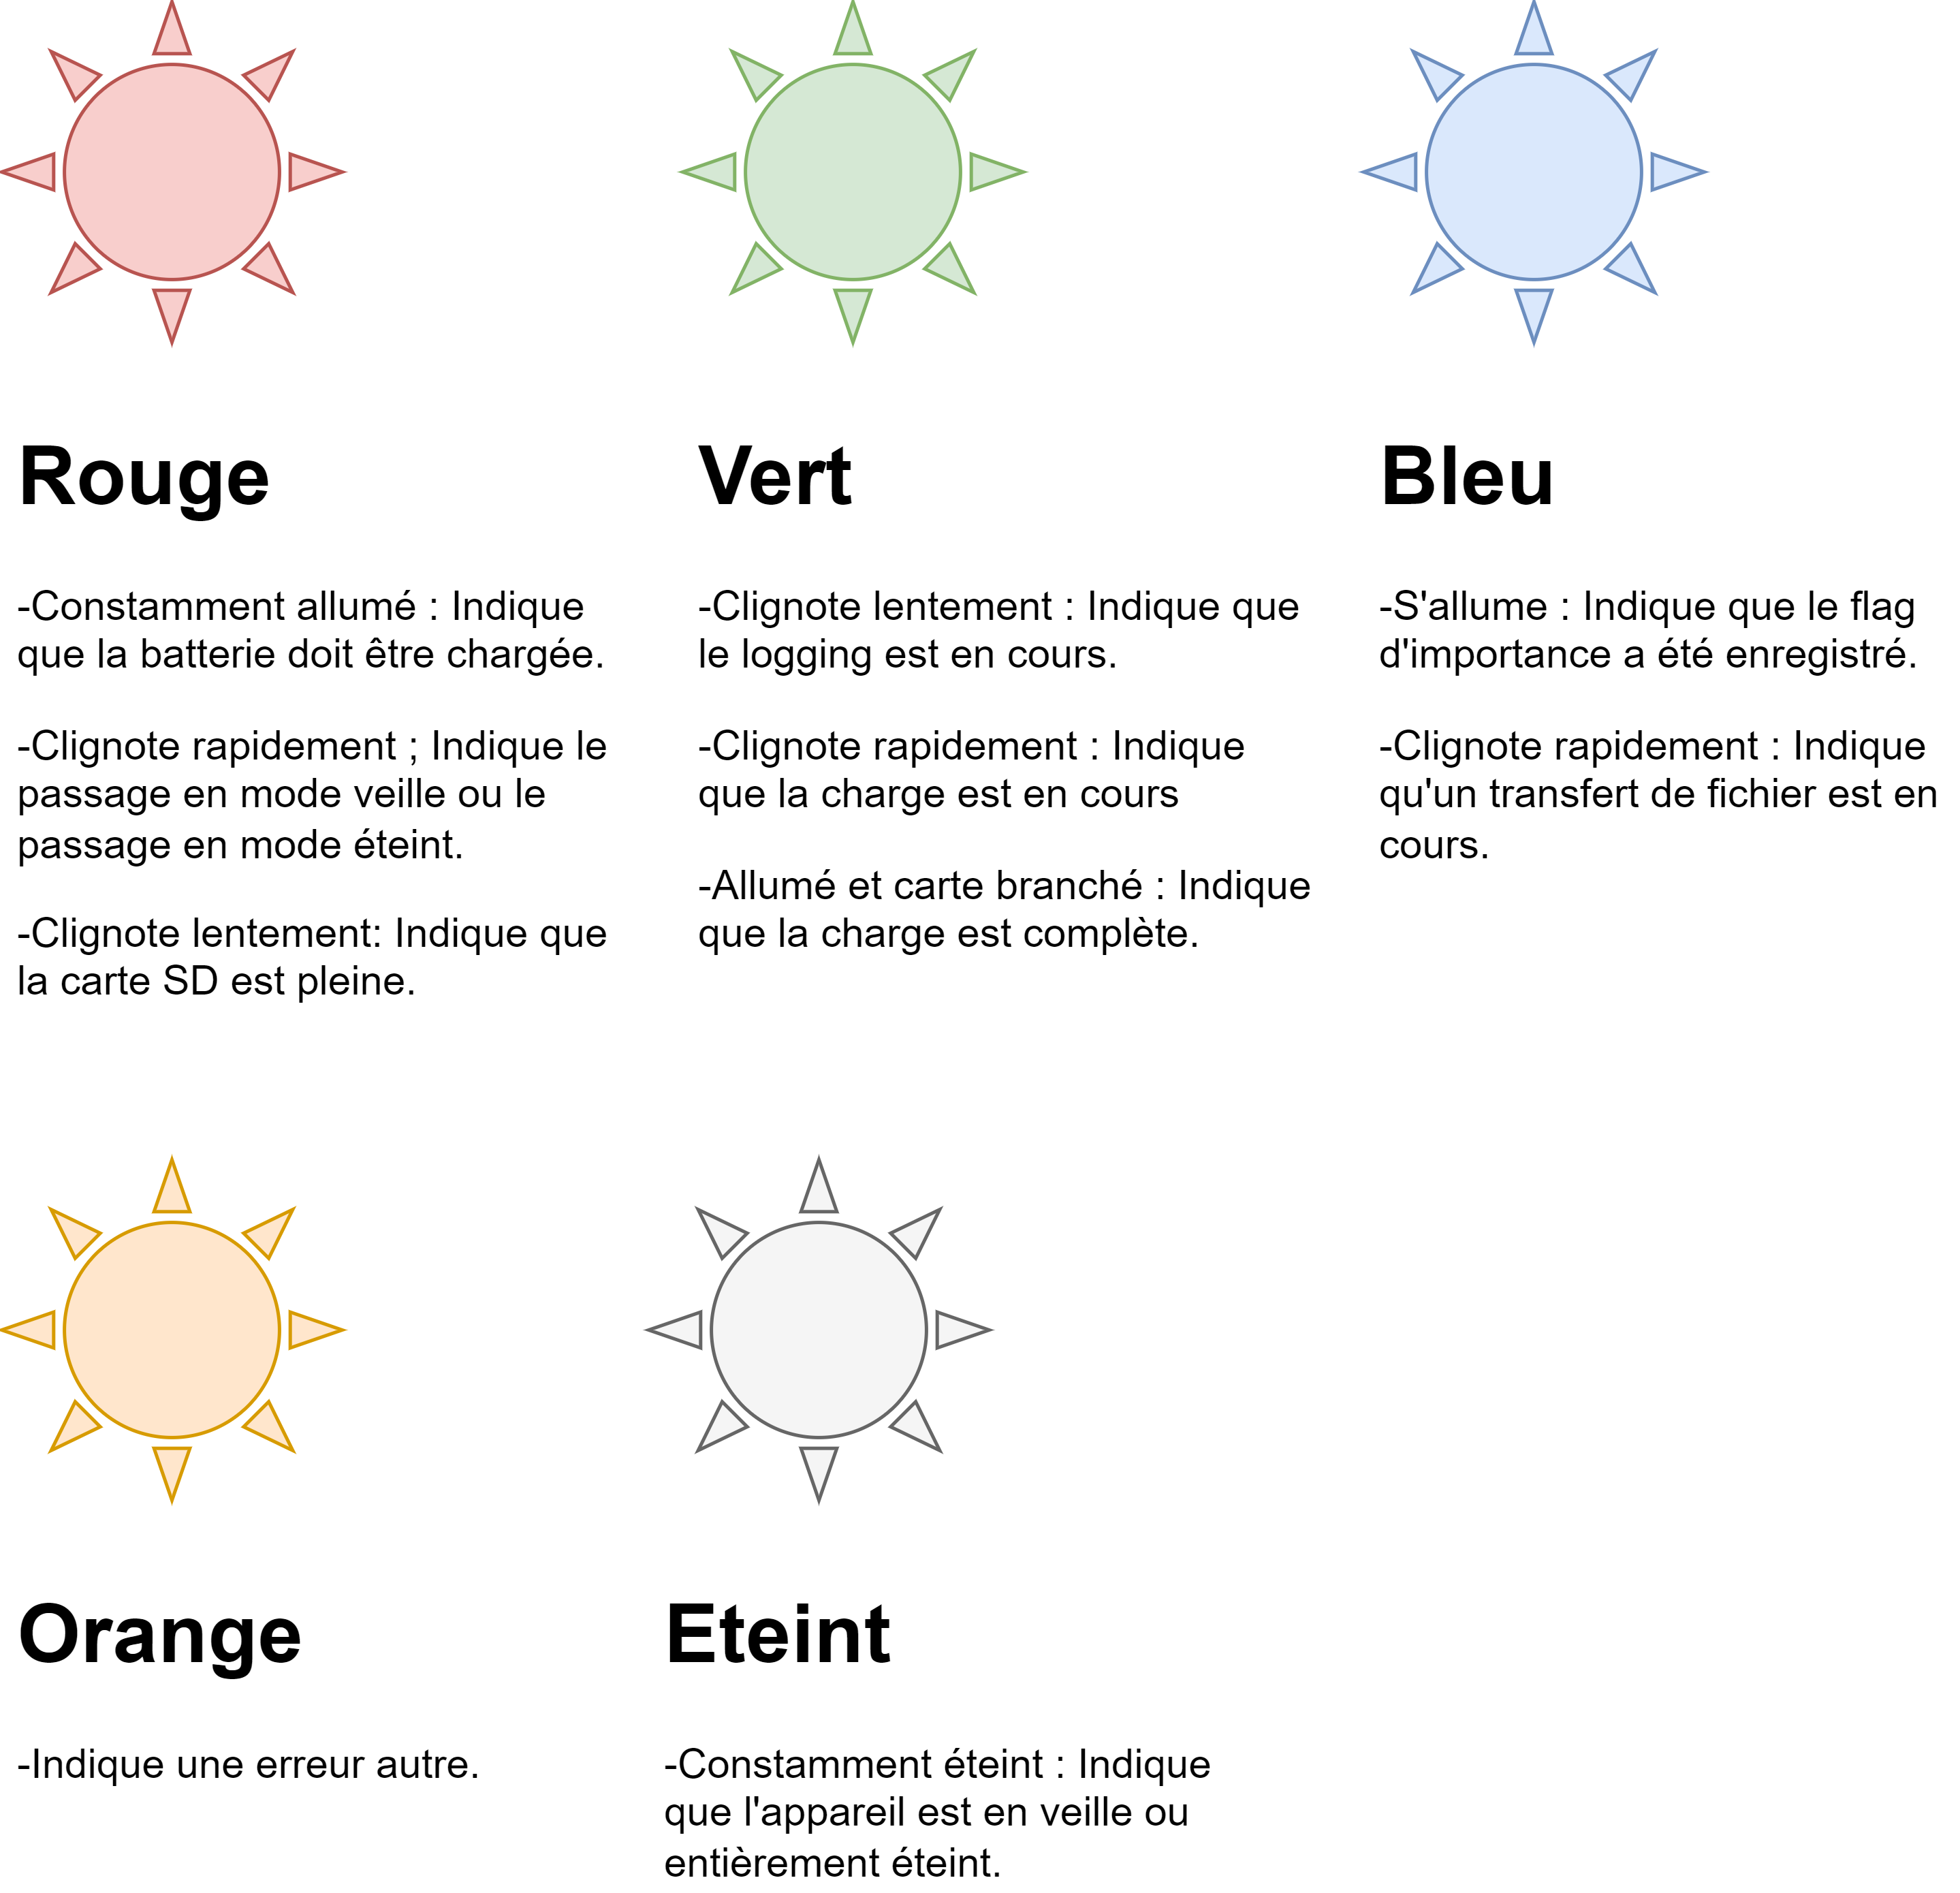
\includegraphics[width=0.95\linewidth]{Figures/Dev-SCH/LEDStates}
			\caption{Définitions des états de la LED RGB}
			\source{Auteur}
			\label{fig:ledstates}
		\end{figure}
	}

	\clearpage
	\subsubsection{Adaptation mécanique} \label{sssec:MecAdapt}
	{	
		L'idée étant d'obtenir une mesure de pression sans modification mécaniques sur le boîtier originale, plusieurs idées ont émergées :
		\begin{itemize}
			\item[1)] Mesurer une déformation mécanique a-même le module, dans le but de déduire la pression (Développement d'un capteur).
			\item[2)] Ajout d'une rallonge cylindrique au module, afin de fixer un capteur de pression à plat sur celui-ci, tout en permettant les modifications mécaniques sans altération du boîtier originale.
		\end{itemize}
		Par sa complexité moins importante et due aux contraintes de temps, la seconde option sera-celle développée lors de cette version du projet.
		Voici des ébauches (Pas à l'échelle) du concept : 
		\begin{figure}[h]
			\centering
			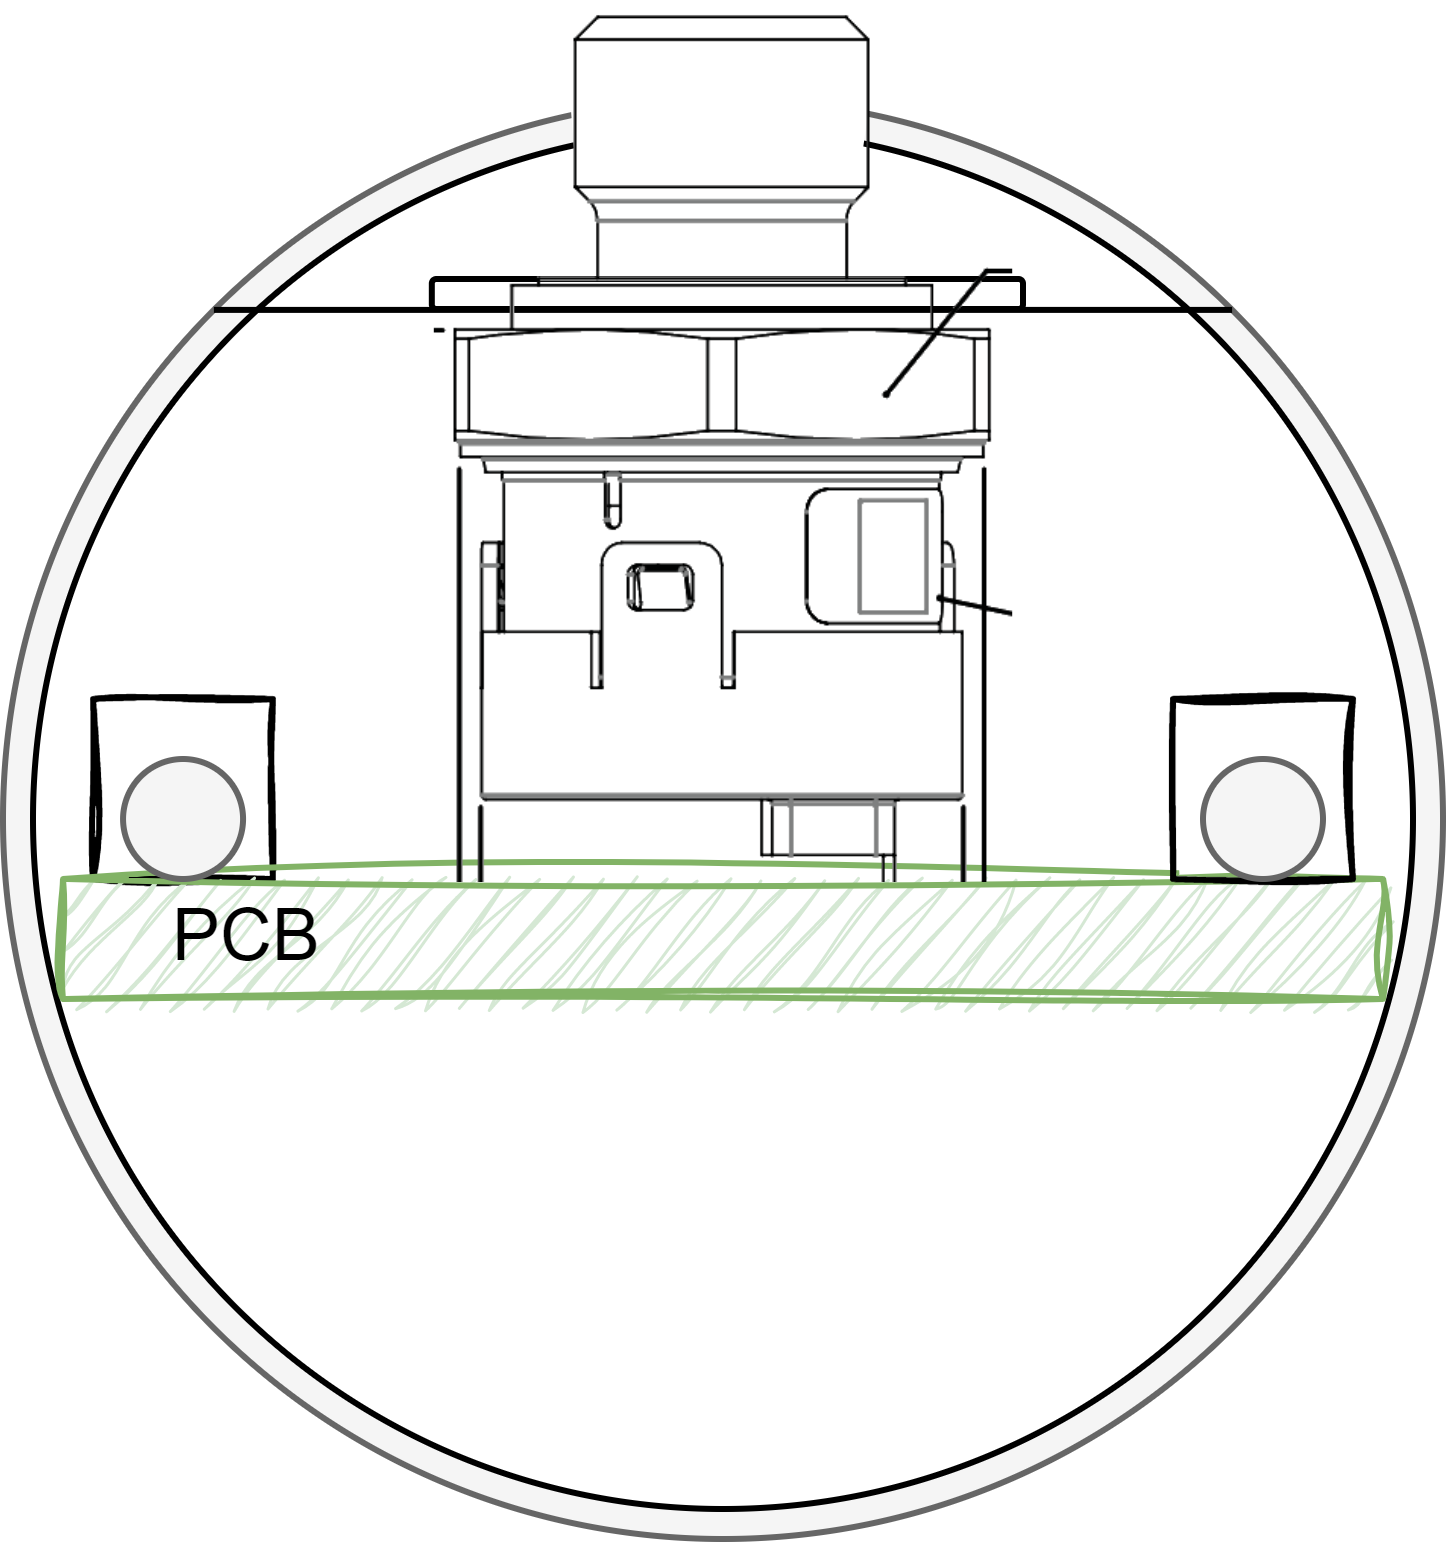
\includegraphics[width=0.45\linewidth]{Figures/Dev-SCH/MecaniqueProto1}
			\caption{Ébauche intérieur du cylindre}
			\label{fig:mecaniqueproto1}
			\source{Auteur}
		\end{figure}\vspace{-5mm}
		\begin{figure}[!h]
			\centering
			
\includegraphics[width=0.75\linewidth]{Figures/Dev-SCH/MecaniqueProto2}
			\caption{Ébauche globale}
			\label{fig:mecaniqueproto2}
			\source{Auteur}
		\end{figure}
		
		
	}

	\clearpage
	\subsubsection{Bus de communications}
	{
		\textbf{UART (1) :} \\
		\underline{Utilisation :} Communication avec les boards Mikroe, pour les clicks-boards utilisant la comm. série. \\
		\underline{Pinning :} \vspace{-6mm}
		\begin{figure}[h]
			\centering
			
\includegraphics[width=0.25\linewidth]{Figures/Dev-SCH/UART1}
			\label{fig:uart1}
		\end{figure}		
	
		\textbf{UART (2) :} \\
		\underline{Utilisation :} Communication avec FTDI conversion USB-Serial. Transfert des fichiers de la carte-SD et mise-à-jour de la RTCC. \\
		\underline{Pinning :} \vspace{-6mm}
		\begin{figure}[h]
			\centering
			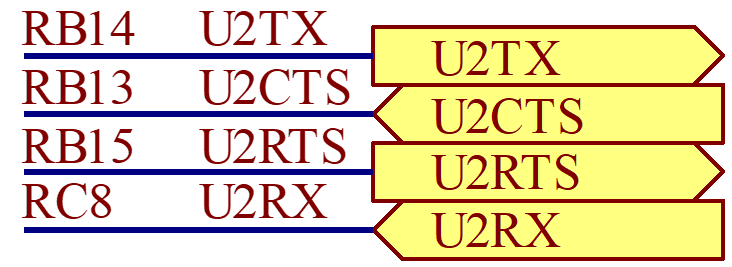
\includegraphics[width=0.25\linewidth]{Figures/Dev-SCH/UART2}
			\label{fig:uart2}
		\end{figure}		
	
		\textbf{SPI :} \\
		\underline{Utilisation :} Communication avec la carte micro-SD, écriture des mesures, timestamps et flag d'importance. \\
		\underline{Pinning :} \vspace{-6mm}
		\begin{figure}[h]
			\centering
			
\includegraphics[width=0.25\linewidth]{Figures/Dev-SCH/SPI}
			\label{fig:spi}
		\end{figure}
	
		\textbf{I2C (1) :} \\
		\underline{Utilisation :} Lecture des mesure de la centrale inertielle BNO055 et paramétrage des registres de celui-ci. \\
		\underline{Pinning :} \vspace{-6mm}
		\begin{figure}[h!]
			\centering
			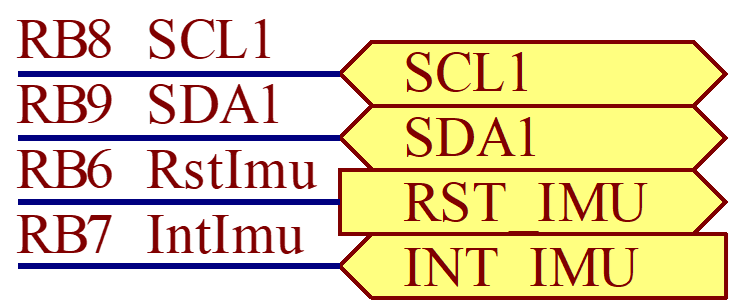
\includegraphics[width=0.25\linewidth]{Figures/Dev-SCH/I2C1}
			\label{fig:i2c1}
		\end{figure}
	
		\textbf{I2C (2) :} \\
		\underline{Utilisation :} Lecture des données du capteur de pression et est également connecté aux slots Mikroe, pour permettre à ceux-ci de communiquer via I2C. \\
		\underline{Pinning :} \vspace{-6mm}
		\begin{figure}[h!]
			\centering
			
\includegraphics[width=0.25\linewidth]{Figures/Dev-SCH/I2C2}
			\label{fig:i2c2}
		\end{figure}
	
		\clearpage
		Pour ce qui est des mesures sur ces différents bus de communications, des connecteurs bergs ont étés prévus, afin de pouvoir connecter facilement un analyseur logique sur les différentes trames : 
		
		\begin{figure}[h]
			\centering
			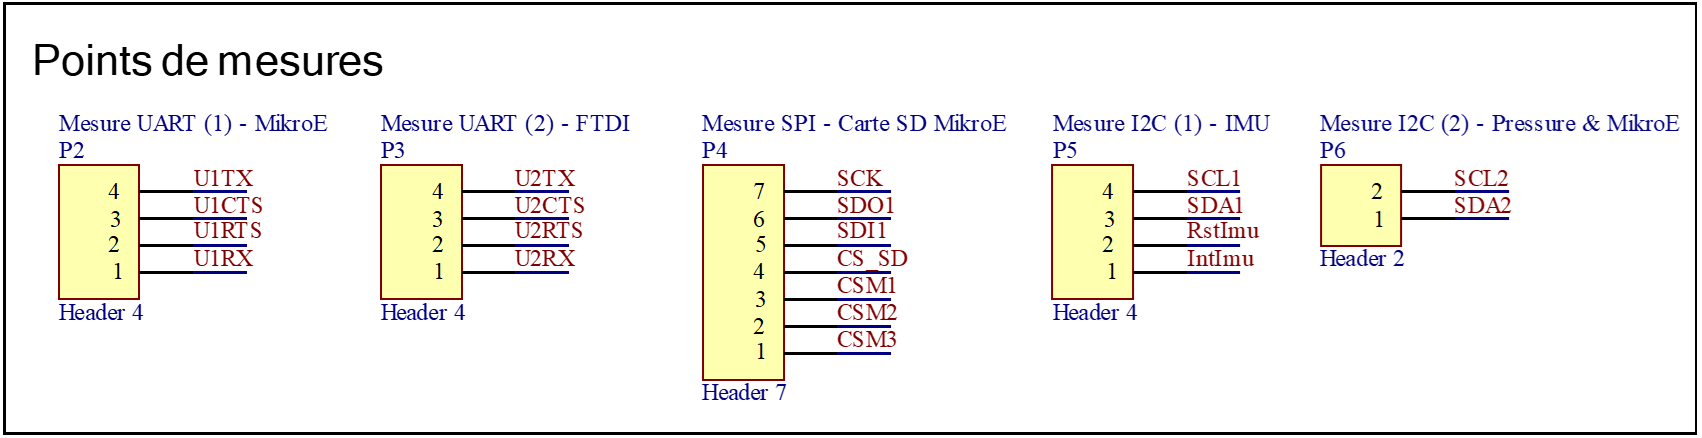
\includegraphics[width=0.9\linewidth]{Figures/Dev-SCH/PointsMesures}
			\caption{Connecteurs pour analyseur logique}
			\label{fig:pointsmesures}
		\end{figure}
		
		Une contrainte s'est crée, lorsque toutes les pins du microcontrôleur ont été allouée alors qu'il restait des connexion pour les "Chip select" et "Reset" des carte click-board Mikroe. Afin de remédier à ce problème, j'ai décidé d'utiliser un démultiplexeur, sachant que chacune des ces PINS, peuvent être activée seulement une à une : 
		
		\begin{figure}[h]
			\centering
			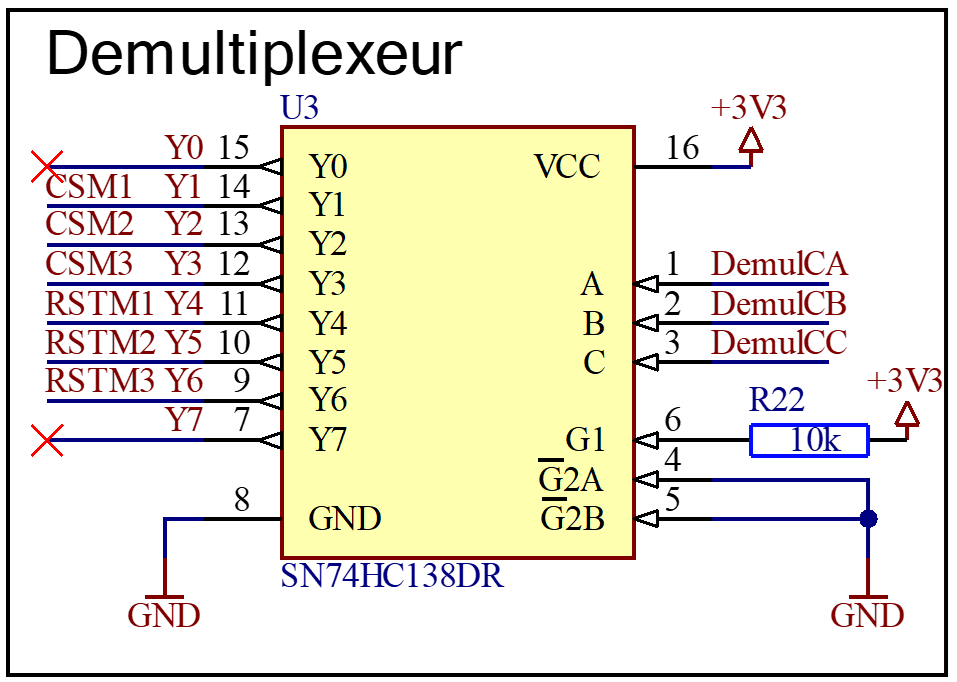
\includegraphics[width=0.6\linewidth]{Figures/Dev-SCH/Demultiplexeur}
			\caption{Demultiplexeur}
			\label{fig:demultiplexeur}
		\end{figure}
	}
	
	\clearpage
	\subsubsection{Périphériques}
	{
		\begin{figure}[h]
			\centering
			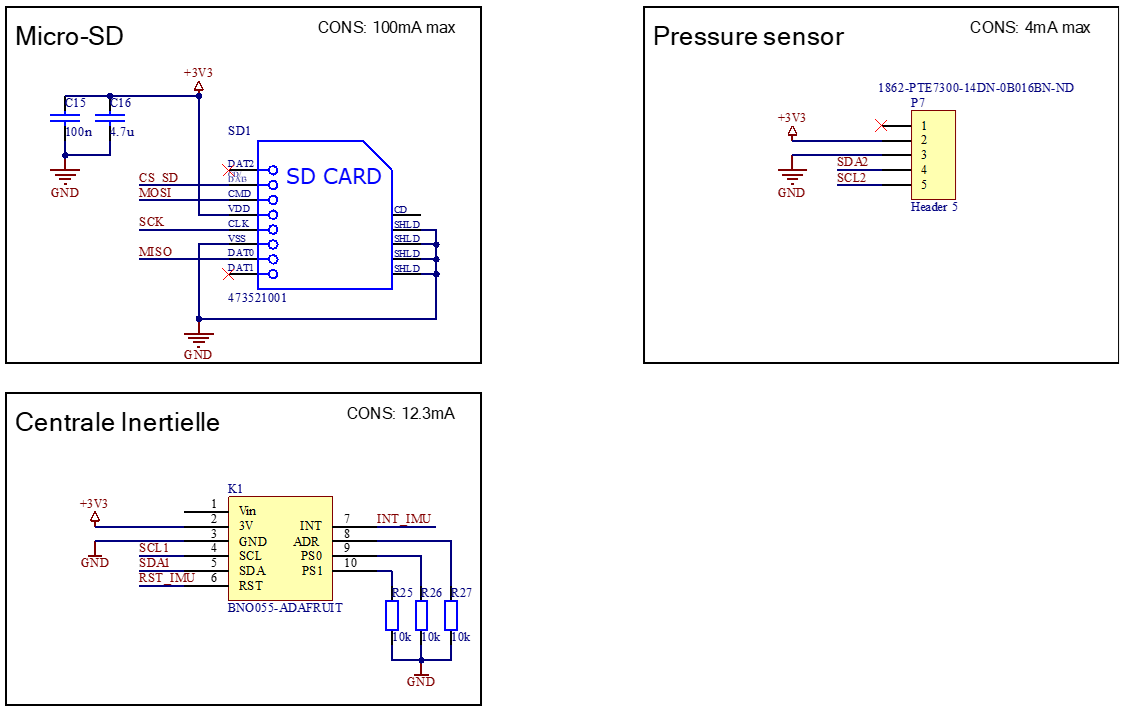
\includegraphics[width=0.85\linewidth]{Figures/Dev-SCH/Periph1}
			\caption{Carte-SD, capteur de pression et centrale inertielle.}
			\label{fig:periph1}
		\end{figure}
		
		Pour la carte-SD, certaines pins ne sont pas utilisée car pas utile dans le cadre du projet (Ex: Pin CD (Card Detect)).
		
		Pour le capteur de pression, il s'agit d'un simple connecteur (AMTEK 5H2001N0-105PXBL00A01) qui vas venir connecter le senseur rattaché à l'extension mécanique.
		
		Quant à la centrale inertielle (BNO055 adafruit-board) le bit d'adresse supplémentaire est mis à 0.
		
		\begin{figure}[h]
			\centering
			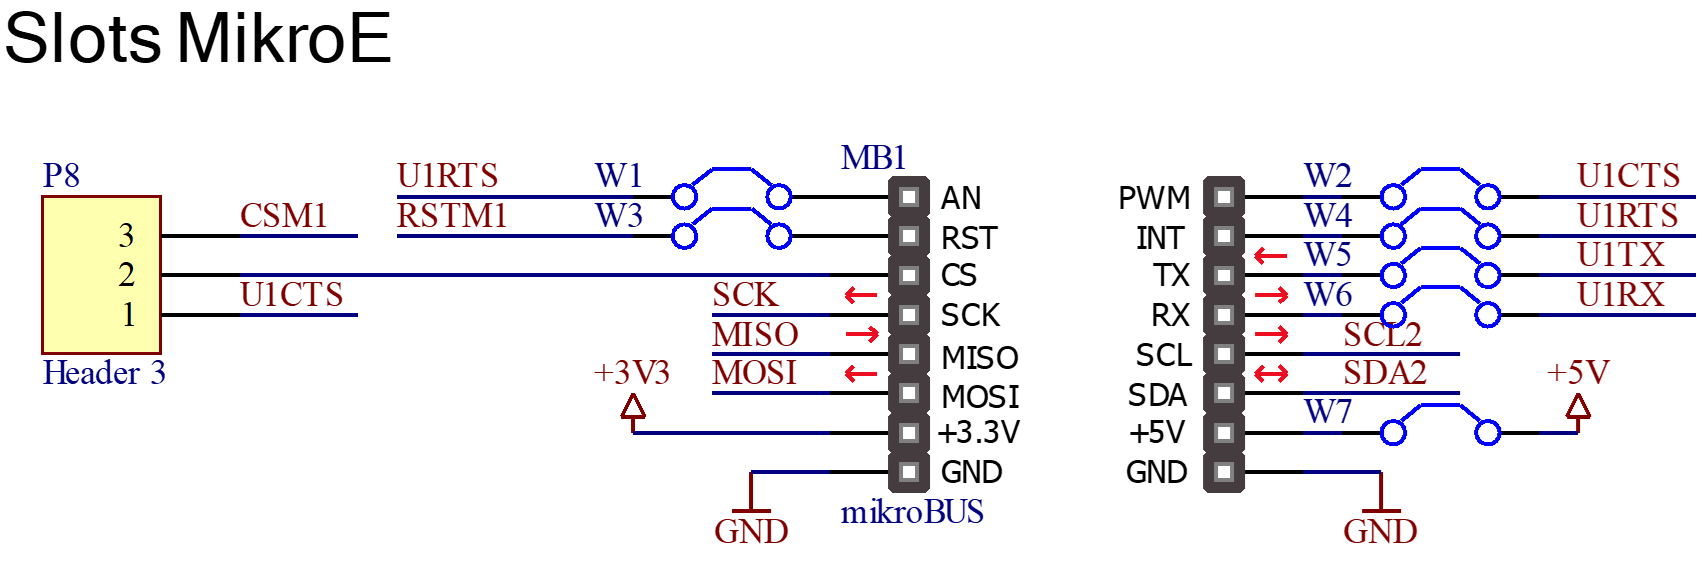
\includegraphics[width=0.8\linewidth]{Figures/Dev-SCH/Mikroe}
			\caption{}
			\label{fig:mikroe}
		\end{figure}
		Les slots Mikroe (3x figure \ref{fig:mikroe}) sont prévus pour pouvoir utiliser le plus de bus de communication possibles. Les jumpers sont prévus pour éviter les collisions sur les lignes.
		
	}

	\clearpage
	\subsubsection{Chargeur de batterie} \label{sssec:BatCharger}
	{
		Ici je vais me pencher sur les dimensionnement des 3 résistances \textit{PROG} du composant de régulation et de charge d'accu, les autres composants passifs n'ont pas requis de dimensionnements particuliers.
		\begin{figure}[h]
			\centering
			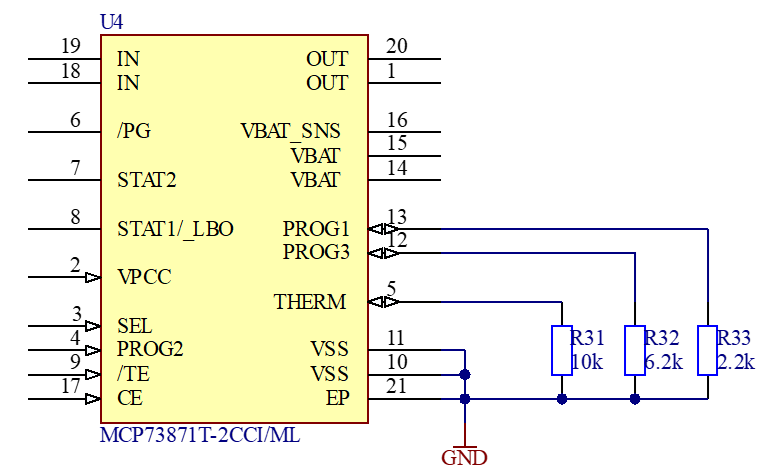
\includegraphics[width=0.55\linewidth]{Figures/Dev-SCH/ChargeBat}
			\caption{IC régulation et gestion charge de l'accu}
			\label{fig:chargebat}
		\end{figure}
		
		Afin de déterminer le comportement de la charge via les différentes étapes de courants, quelques équations ont été utiles : \\
		Où \\
		$C = 3400mAh$ \\
		$ratio_{term} = 0.05$
		$ratio_{chrg} = 0.1$
		
		\begin{equation} \label{equ:ich}
			I_{term} = C * ratio_{chrg} 
		\end{equation}
		D'après \ref{equ:ich}, $I_{term} = 170mA$.
	 
	 	\begin{equation} \label{equ:Rprog3}
		 	Rprog3 = \frac{1000V}{I_{term}}
		\end{equation}
		D'après \ref{equ:Rprog1}, $Rprog3 = 5k88 \Omega$ E12 $\Longrightarrow$ $6k2\Omega$ (Arrondis au supérieur pour limiter courant de terminaison).
		
		\begin{equation} \label{equ:Rprog1}
			Rprog1 = \frac{1000V}{C * ratio_{chrg}} 
		\end{equation}
		D'après \ref{equ:Rprog1}, $Rprog1 = 2k94 \Omega$ E12 $\Longrightarrow$ $2k2\Omega$ (Arrondis à l'inférieur pour limiter courant de charge).
		 
	}
	
	\clearpage
	\subsubsection{Conclusion et perspectives} \label{sssec:MethSchematic}
	{
		Lors du développement de la schématique, je n'ai pas eu de grands dimensionnements à faire mais plutôt dû mettre en place des mécanismes permettant la communication avec tous les senseurs et périphériques du système. J'ai essayé d'être le plus explicite possible lors de la création des différents blocs du schéma électrique, pour permettre une compréhension aisée de celui-ci. 
		
		J'ai pû faire un contrôle mutuel de la schématique avec mon collègue M. Meven Ricchieri.
		
		Je n'ai pas rencontré de problèmes particuliers, j'ai pus compléter la schématique, avancer sur le concept globale et je suis très enthousiaste de continuer ce projet.
		
		Désormais il vas falloir préparer la création du PCB, en contrôlant les footprints du circuit et développer d'avantage l'aspect mécanique du projet.
		
		La schématique issue de cette partie développement,  sera disponible en annexe de ce rapport.
		
		
	}
	

}


\clearpage

% ---------- DÉVELOPPEMENT PCB ----------------------------- 
% ------------------------- MAIN TASK ---------------------------------
\section{Développement du PCB}

\subsection{Footprints} \label{ssec:Footprints}
{}
\clearpage

\subsection{Bill of materials} \label{ssec:BOM}
{}
\clearpage

\subsection{Mécanique du projet} \label{ssec:mechProjet}
{}
\clearpage

\subsection{Restrictions mécaniques} \label{ssec:RestrictionMech}
{}
\clearpage

\subsection{Planification PCB} \label{ssec:planifPCB}
{}
\clearpage

\subsection{Placement des composants} \label{ssec:placementComp}
{}
\clearpage

\subsection{Routage} \label{ssec:routage}
{}
\clearpage

% ---------- DÉVELOPPEMENT SOFTWARE ----------------------------- 
% !TeX spellcheck = fr_FR
\section{Développement firmware}
Dans cette section, nous allons décrire et expliquer le processus de programmation du code qui a été implémenté dans le microcontrôleur PIC32MX130F256D.
Le processus de programmation du code dans le PIC32MX130F256D comprend plusieurs étapes. Tout d'abord, il est nécessaire de disposer d'un environnement de développement intégré (IDE) adapté à ce microcontrôleur, tel que MPLAB X IDE. Cet IDE est équipé de l'environnement Harmony, qui permet l'utilisation d'un configurateur graphique pour les différentes bibliothèques du PIC.

\subsection{Configuration des PINs dans Harmony}
{
	\begin{figure}[h]
		\centering
		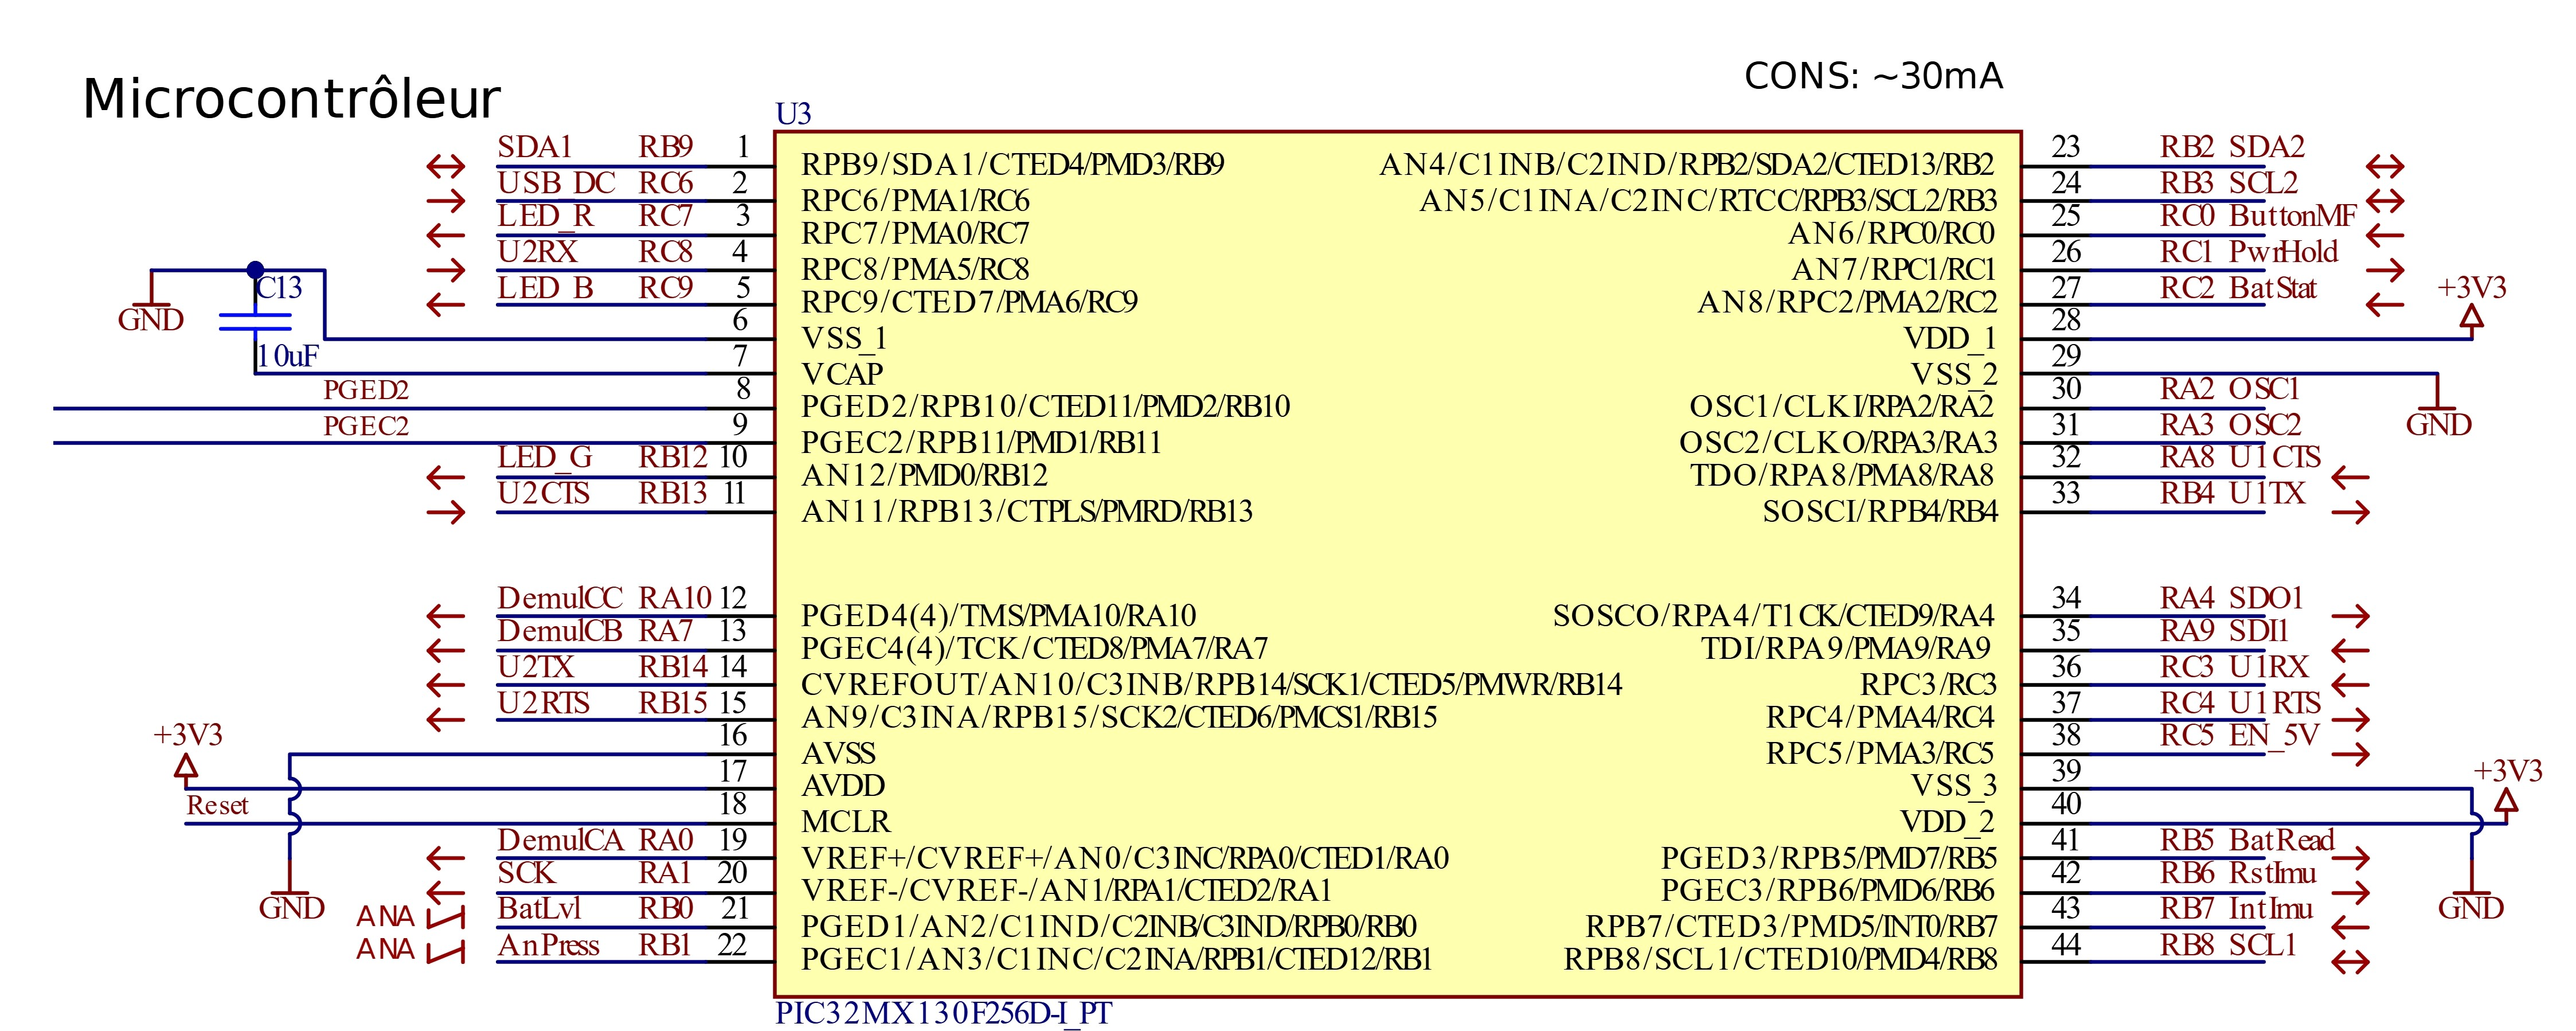
\includegraphics[width=.9\textwidth]{Figures/Dev-SOFT/MCU-Altium}
		\caption{Pinning réelles dans altium designer}
		\label{fig:mcu-altium}
	\end{figure}
	\begin{figure}[h]
		\centering
		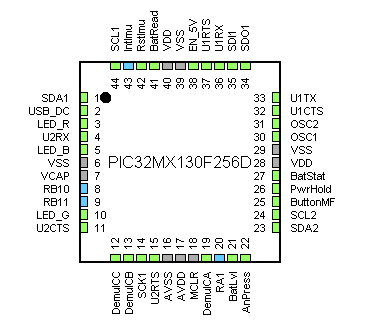
\includegraphics[width=0.5\textwidth]{Figures/Dev-SOFT/MCU-Harmony}
		\caption{Pinning dans Harmony}
		\label{fig:mcu-harmony}
	\end{figure}
	
	On peut constater que la PIN 20 (SCK) est en haute impédance dans Harmony, tandis que la PIN 14, qui était supposée être \textit{U2TX}, est maintenant configurée en tant que SCK. Cela est dû à une erreur : SCK ne peut être assigné qu'à la PIN 14. Par conséquent, il a été nécessaire d'ajouter un fil externe pour relier la PIN 14 à la PIN 20, ce qui a entraîné la perte de la communication USB sur l'UART2. Cette modification sera expliquée en détail ultérieurement.
	
	
}

\subsection{Configuration des périphériques dans Harmony}
{
	\subsubsection{Timers} 
	
	Deux timers seront utilisés, l'un pour mesurer des attentes en ms et l'autre moins rapide, pour les diverses actions du programmes, avec une interruptions chaque 10ms.
	\begin{table}[h]
		\centering
		\begin{tabular}{|l|l|}
			\hline
			Timer & Temps voulu \\
			\hline
			Timer 1 & 1ms \\
			\hline
			Timer 2 & 10ms \\
			\hline
		\end{tabular}
	\end{table}

	La fréquence de l'horloge système a été augmentée à 48 MHz dans le but d'accélérer l'ensemble du système, étant donné qu'il implique de nombreuses communications nécessitant des opérations rapides, que ce soit pour la préparation des tampons de données ou les divers calculs.
	
	\begin{figure}[h]
		\centering
		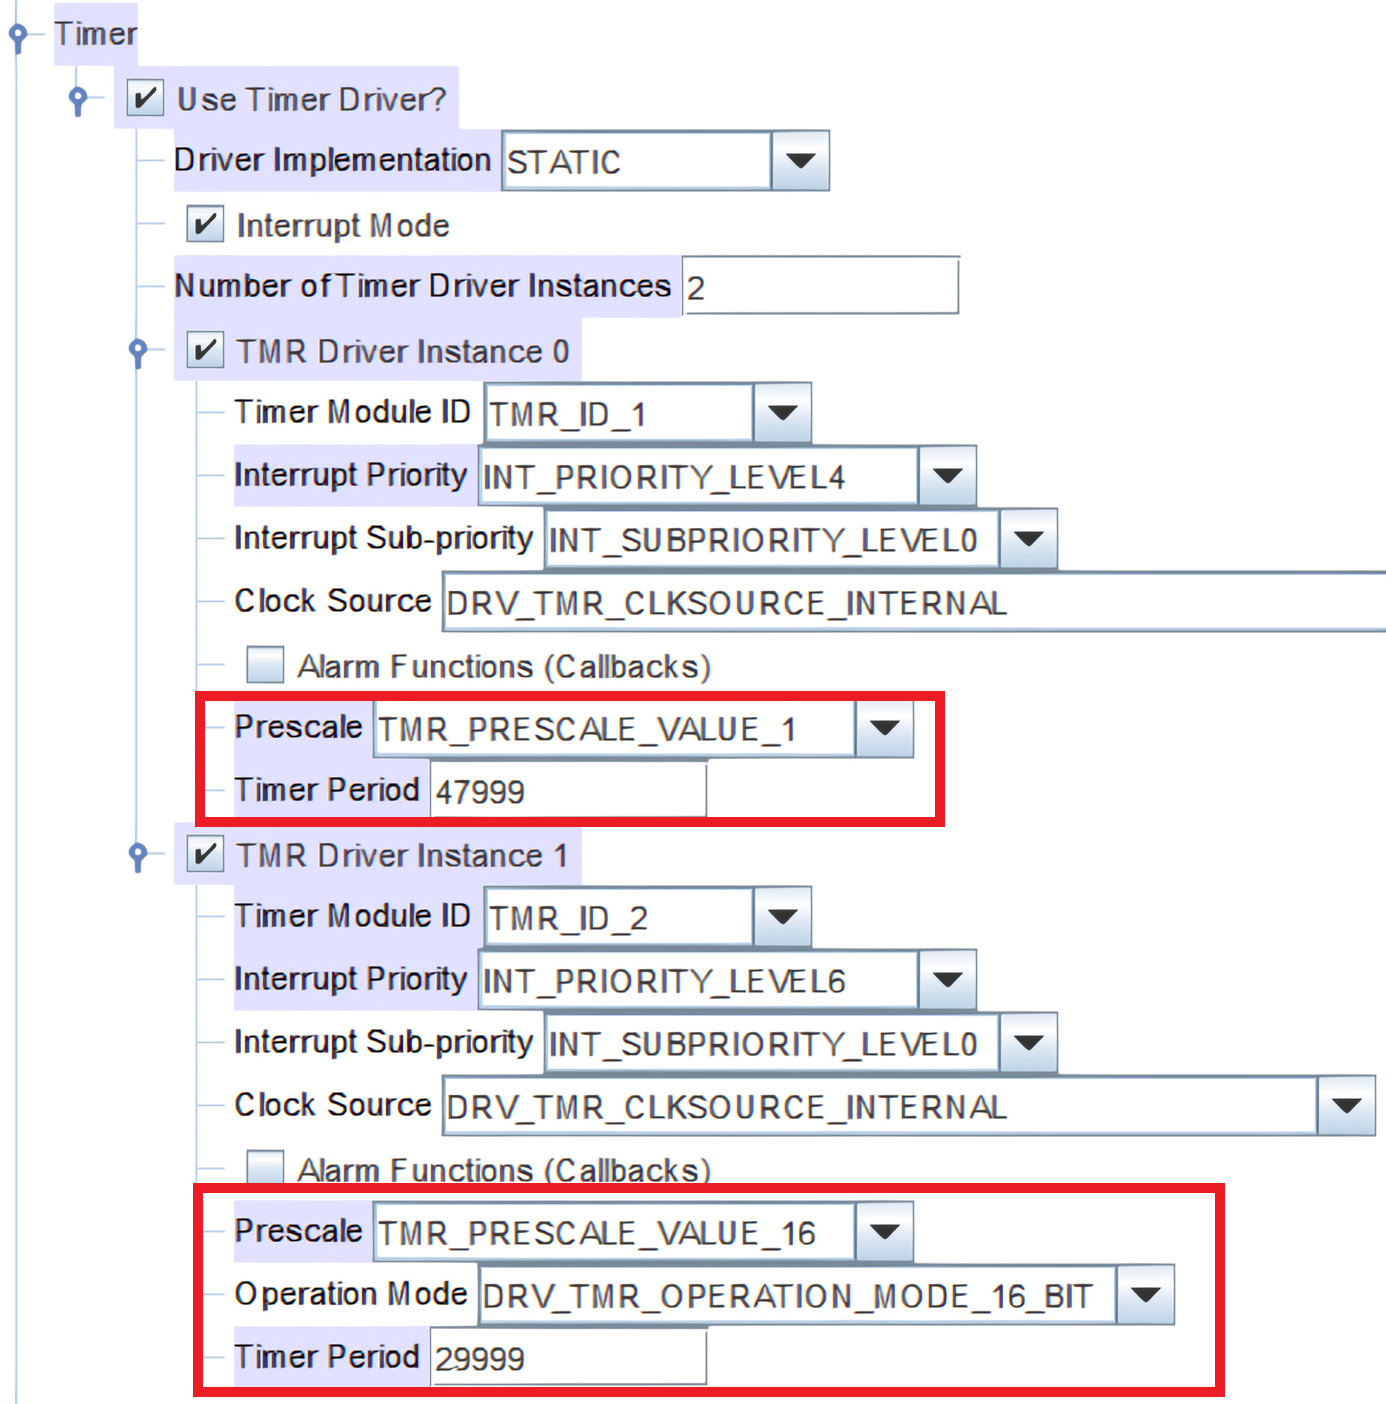
\includegraphics[width=0.55\linewidth]{Figures/Dev-SOFT/Timer_config}
		\caption{Configuration dans harmony}
		\label{fig:timerconfig}
	\end{figure}

	\begin{figure}[h]
		\centering
		\begin{subfigure}[b]{0.45\textwidth}
			\centering
			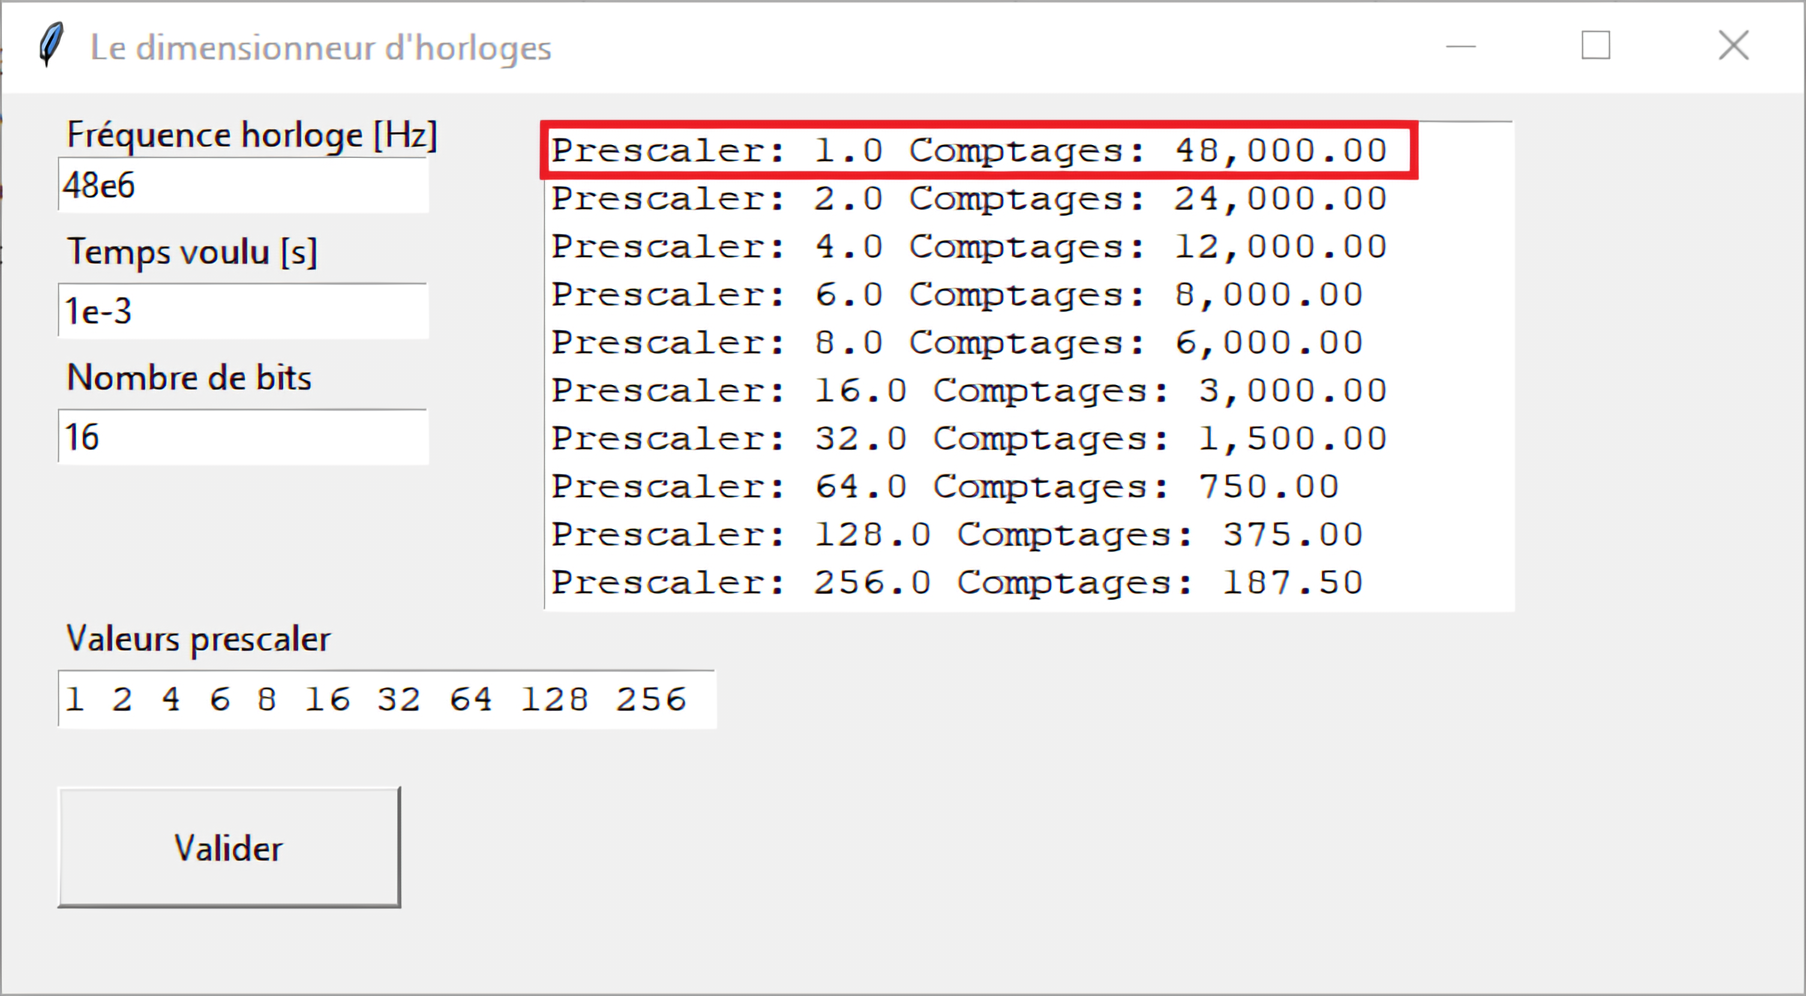
\includegraphics[width=\textwidth]{Figures/Dev-SOFT/Timer1ms}
			\caption{Timer 1, Dimensionnement pour 1ms}
			\label{fig:timer1ms}
		\end{subfigure}
		\hfill
		\begin{subfigure}[b]{0.45\textwidth}
			\centering
			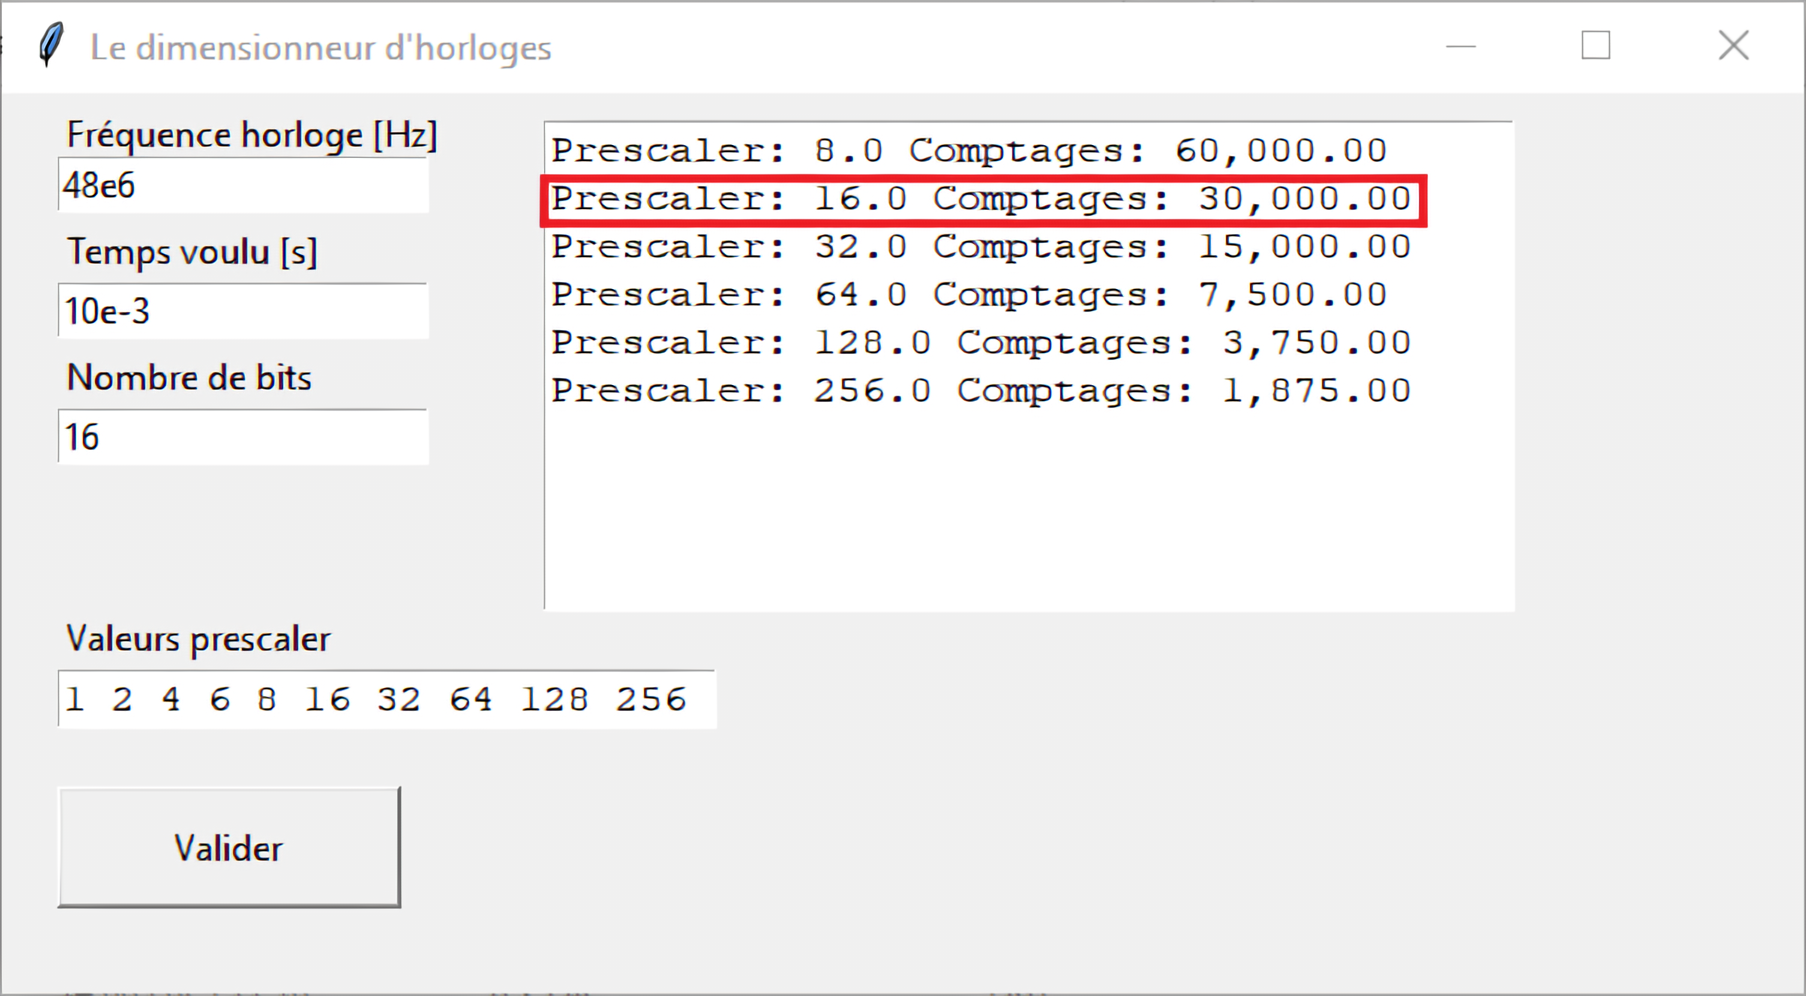
\includegraphics[width=\textwidth]{Figures/Dev-SOFT/Timer10ms}
			\caption{Timer 2, Dimensionnement pour 10ms}
			\label{fig:timer10ms}
		\end{subfigure}
		\hfill
		\caption{Application timer développée par l'auteur}
		\label{fig:appTimer}
	\end{figure}

	\clearpage

	\subsubsection{USART} \label{ssec:Usart}
	Dans le but de vérifier les données de mesure en temps réel et de faciliter le débogage, une communication sérielle UART a été mise en place. Pour cela, le périphérique UART1, initialement prévu pour le slot mikroe, a été utilisé. Un module USB-to-TTL externe sera utilisé pour lire les données via Putty sur un ordinateur.
	
	\begin{figure}[h]
		\centering
		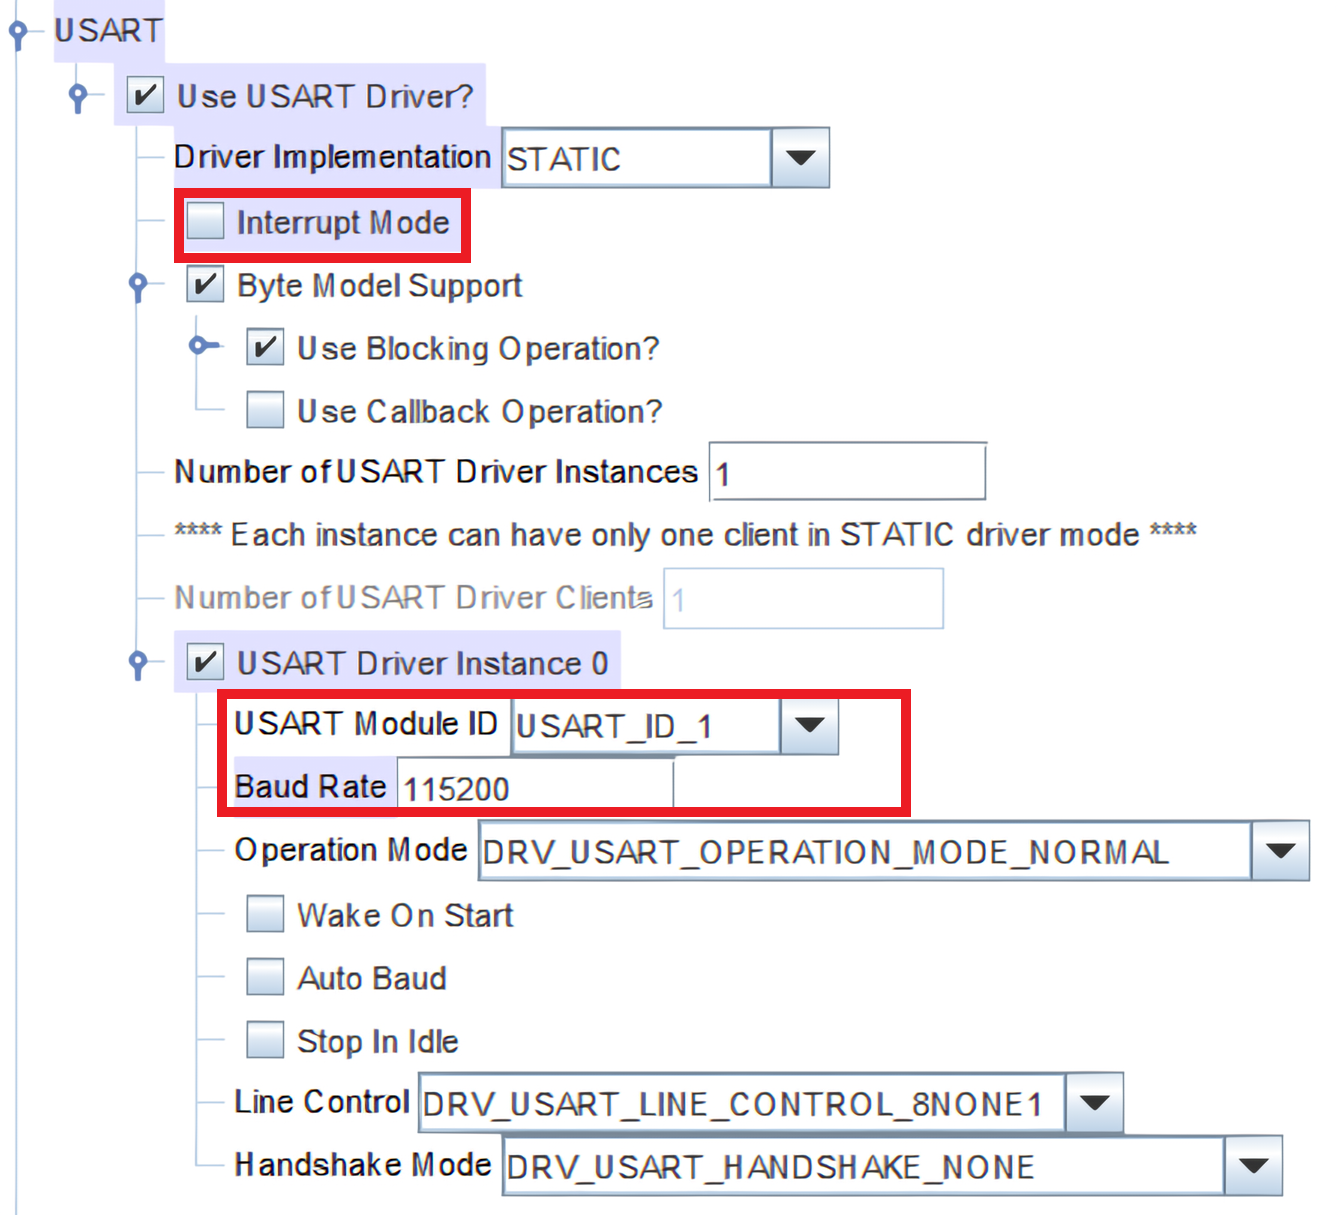
\includegraphics[width=0.7\linewidth]{Figures/Dev-SOFT/ConfigUart}
		\caption{Configuration UART}
		\label{fig:configuart}
	\end{figure}
	
	
	Nous pouvons constater sur la figure \ref{fig:configuart} que l'UART est configuré sans interruption à un bauderate de 115200.

	\subsubsection{Carte SD - SPI} 
	{
	L'utilisation du SPI a été optimisée en choisissant une fréquence de 5 MHz afin de réduire le temps d'exécution sur le microcontrôleur, compte tenu du grand nombre de trames nécessaires pour les opérations FAT. Cependant, j'ai rencontré un problème lié à la clock du SPI. En raison de la vitesse élevée et des modifications que j'ai dû apporter, la clock interfère inutilement avec le FTDI, et un fil relie SCK et U2TX, créant ainsi une inductance parasite. Pour résoudre ce problème, j'ai ajouté un condensateur de \textbf{33pF} entre SCK et GND pour stabiliser la communication. Vous pouvez consulter la configuration Harmony de la carte SD sur la figure \ref{fig:configsdspi}.
	\clearpage
	\begin{figure}[h]
		\centering
		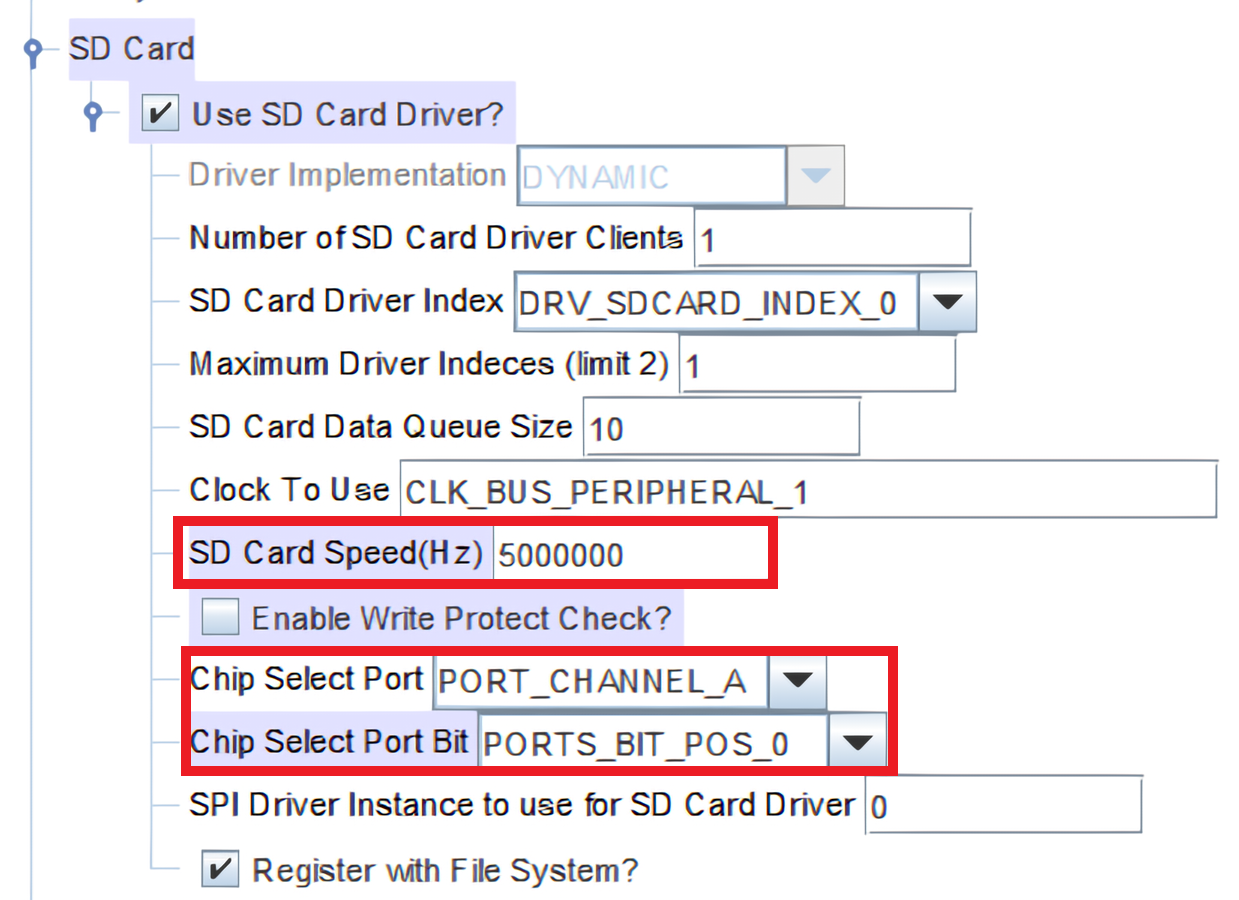
\includegraphics[width=0.7\linewidth]{Figures/Dev-SOFT/ConfigSD_SPI}
		\caption{Configuration du SPI}
		\label{fig:configsdspi}
	\end{figure}
	}

	\subsection{Code}
	Je vais dans cette section décrire le code du projet. Voici la hiérarchie des fichier du projet :
	\begin{figure}[h]
		\centering
		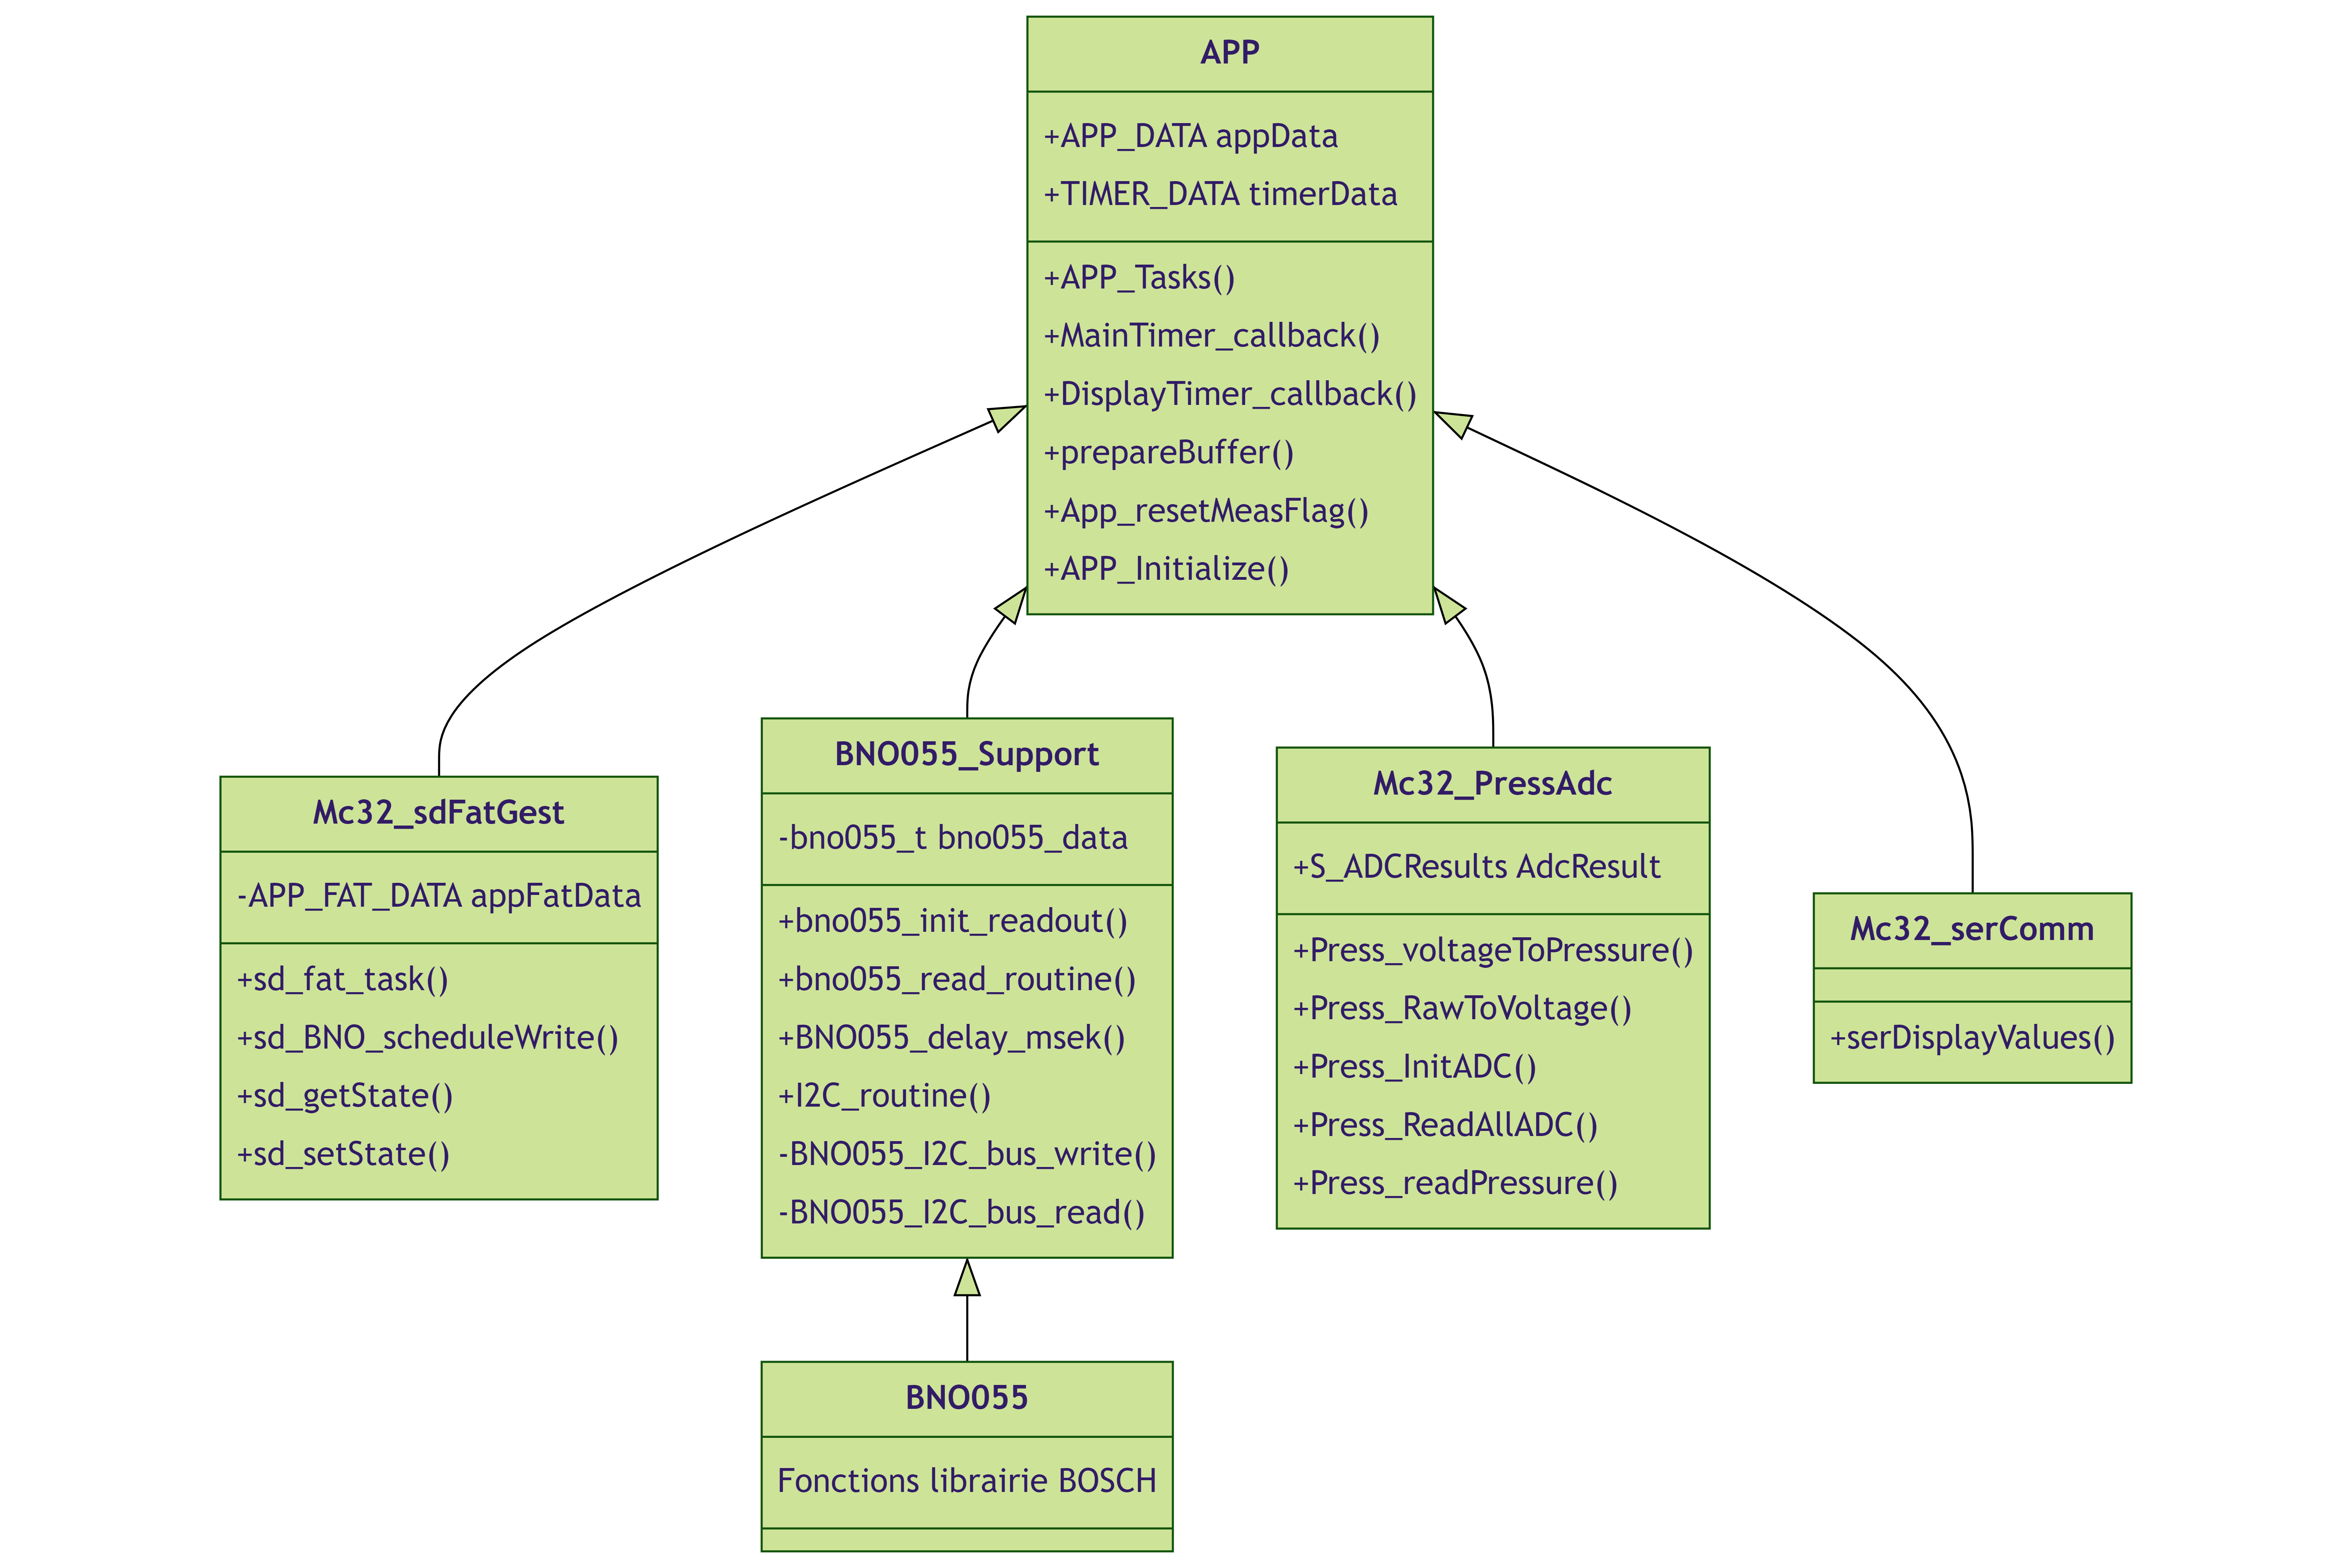
\includegraphics[width=0.79\linewidth]{Figures/Dev-SOFT/ClassesCode}
		\caption{Hiérarchie des fichiers du projet}
		\label{fig:classescode}
	\end{figure}
	
	\clearpage	
	
	\subsubsection{Callbacks}
	{
	Chacun des timers appelle dans leur interruption une fonction appartenant au fichier \textit{app.c}, qui contient les actions définies pour chaque intervalle de temps spécifique. On peut visualiser cela sur le diagramme présenté dans la figure \ref{fig:callbacks}.
	
	\begin{figure}[h!]
		\centering
		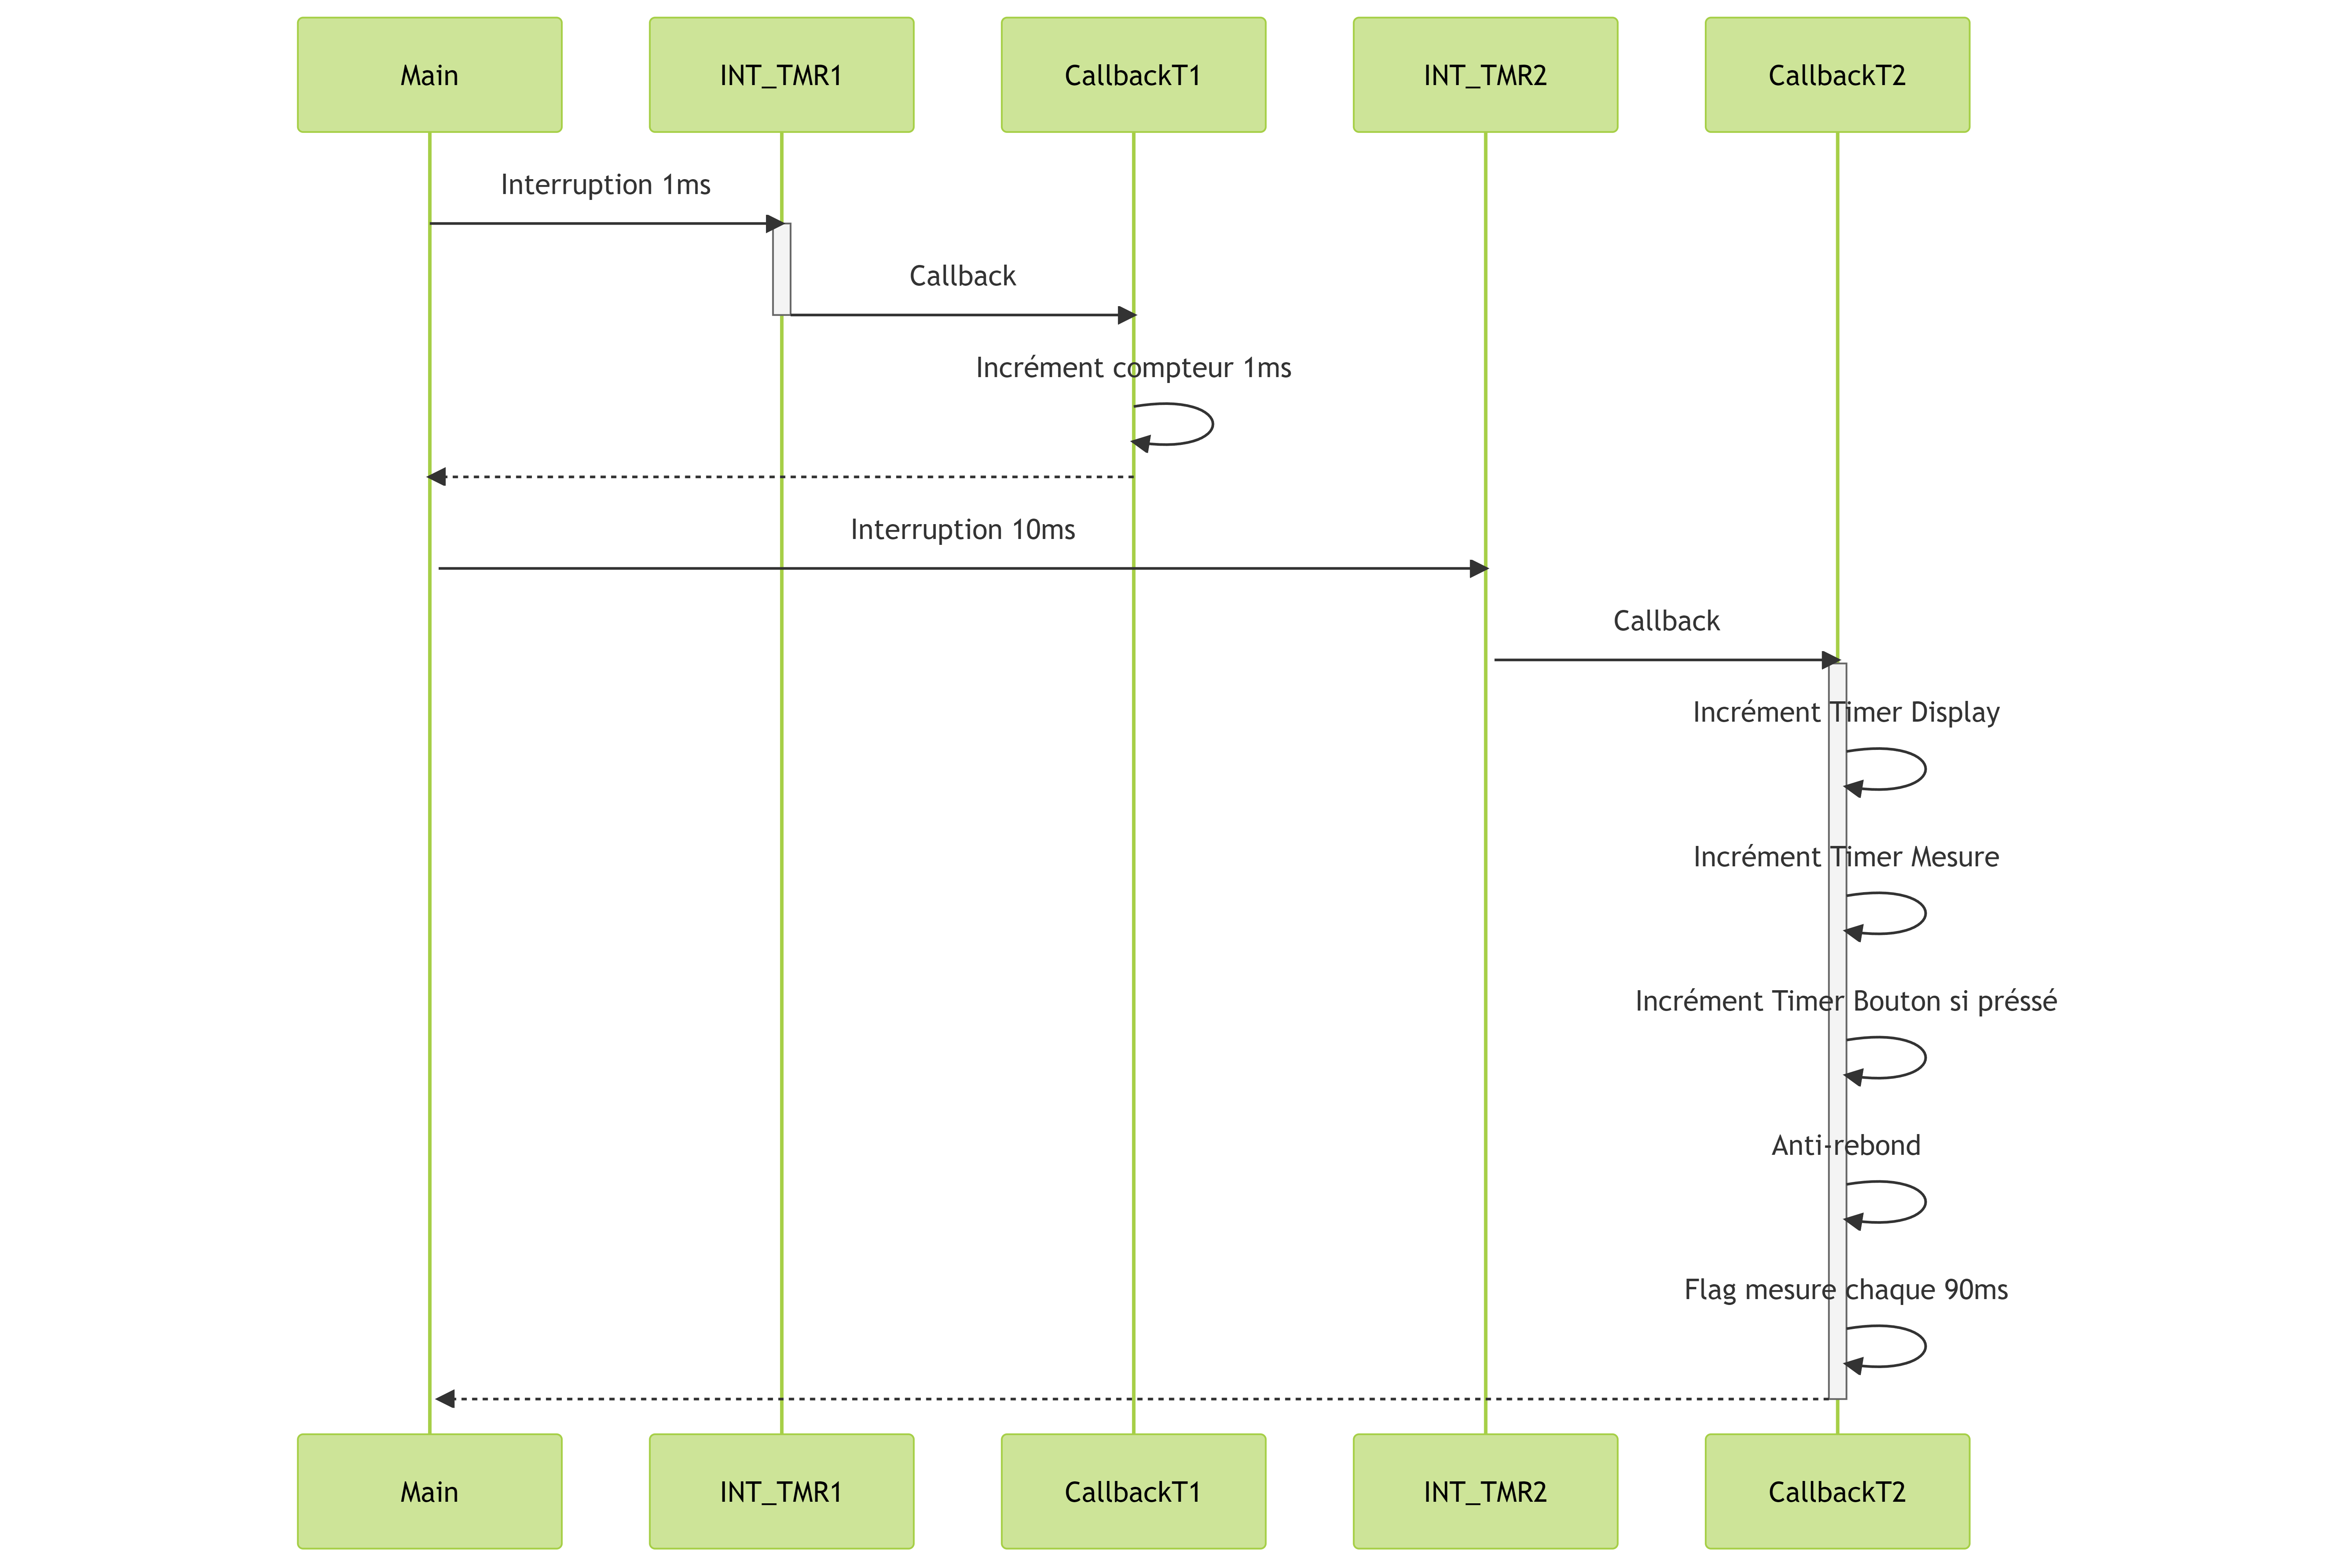
\includegraphics[width=1\textwidth]{Figures/Dev-SOFT/Callbacks}
		\caption{Interactions des interruptions et des callbacks}
		\label{fig:callbacks}
	\end{figure}

	Les callbacks en C offrent flexibilité, extensibilité et réutilisabilité. Ils permettent d'ajuster dynamiquement le comportement du programme, d'étendre les fonctionnalités et de réutiliser le code. Les callbacks favorisent également l'encapsulation et la personnalisation, améliorant ainsi la modularité et la maintenance du code.	
	}
	
	\clearpage
	\subsubsection{Centrale inertielle BNO055}
	Pour ce qui est de la centrale inertielle BNO055, j'ai utilisé la bibliothèque de BOSCH \footnote{\href{https://github.com/BoschSensortec/BNO055_driver}{Bibliothèque du fabricant}}. Je l'ai configurée en 32 bits et j'ai créé les fonctions de bas niveau (i2c) en établissant le lien avec la bibliothèque BOSCH. Tout cela a été fait dans le fichier BNO055\_support.c.
	
	Pour faire le lien entre la bibliothèque de haut niveau et la bibliothèque de bas niveau, j'ai utilisé un pointeur de fonction présent dans la structure de données du BNO, comme illustré dans le listing \ref{lst:lienPointeur}.
	
\begin{lstlisting}[frame=single, label={lst:lienPointeur}, language=C, caption={Code lien pointeur de fonction}, captionpos=b]
s8 I2C_routine(void)
{
	bno055.bus_write = BNO055_I2C_bus_write;
	bno055.bus_read = BNO055_I2C_bus_read;
	bno055.delay_msec = BNO055_delay_msek;
	bno055.dev_addr = BNO055_I2C_ADDR1;
	return BNO055_INIT_VALUE;
}
\end{lstlisting}
\begin{lstlisting}[frame=single, language=C, caption={Code écriture i2c au BNO055}, captionpos=b, breaklines=true]
s8 BNO055_I2C_bus_write(u8 dev_addr, u8 reg_addr, u8 *reg_data, u8 cnt)
{
	s8 BNO055_iERROR = BNO055_INIT_VALUE;
	u8 array[I2C_BUFFER_LEN];
	u8 stringpos = BNO055_INIT_VALUE;
	array[BNO055_INIT_VALUE] = reg_addr;
	
	i2c_start();
	BNO055_iERROR = i2c_write(dev_addr<<1);
	
	for (stringpos = BNO055_INIT_VALUE; stringpos < (cnt+BNO055_I2C_BUS_WRITE_ARRAY_INDEX); stringpos++)
	{
		BNO055_iERROR = i2c_write(array[stringpos]);
		array[stringpos + BNO055_I2C_BUS_WRITE_ARRAY_INDEX] = *(reg_data + stringpos);
	}
	
	i2c_stop();
	if(BNO055_iERROR-1 != 0)
		BNO055_iERROR = -1;
	else
		BNO055_iERROR = 0;
	return (s8)(BNO055_iERROR);
}
\end{lstlisting}
	Pour ce qui est de l'utilisation de la libraire haut-niveau bno055\_support, voici la préparation et la lecture des données : 
	
	\begin{lstlisting}[frame=single, language=C, caption={Code lecture des données par la librairie}, captionpos=b, breaklines=true]
/* BNO055 Read all important info routine */
bno055_local_data.comres = bno055_read_routine(&bno055_local_data);
/* Delta time */
bno055_local_data.d_time = timerData.TmrMeas - timerData.ltime;
/* Pressure measure */
bno055_local_data.pressure = Press_readPressure();
/* Flag measure value */
bno055_local_data.flagImportantMeas = flagMeas;
	\end{lstlisting}

	\subsubsection{Carte SD}
	La  communication de la carte SD fonctionne sous forme d'une machine d'état non-bloquante, permettant ainsi de s'adapter aux situations de la carte sans bloquer le système pour autant.
	
	\begin{figure}[h]
		\centering
		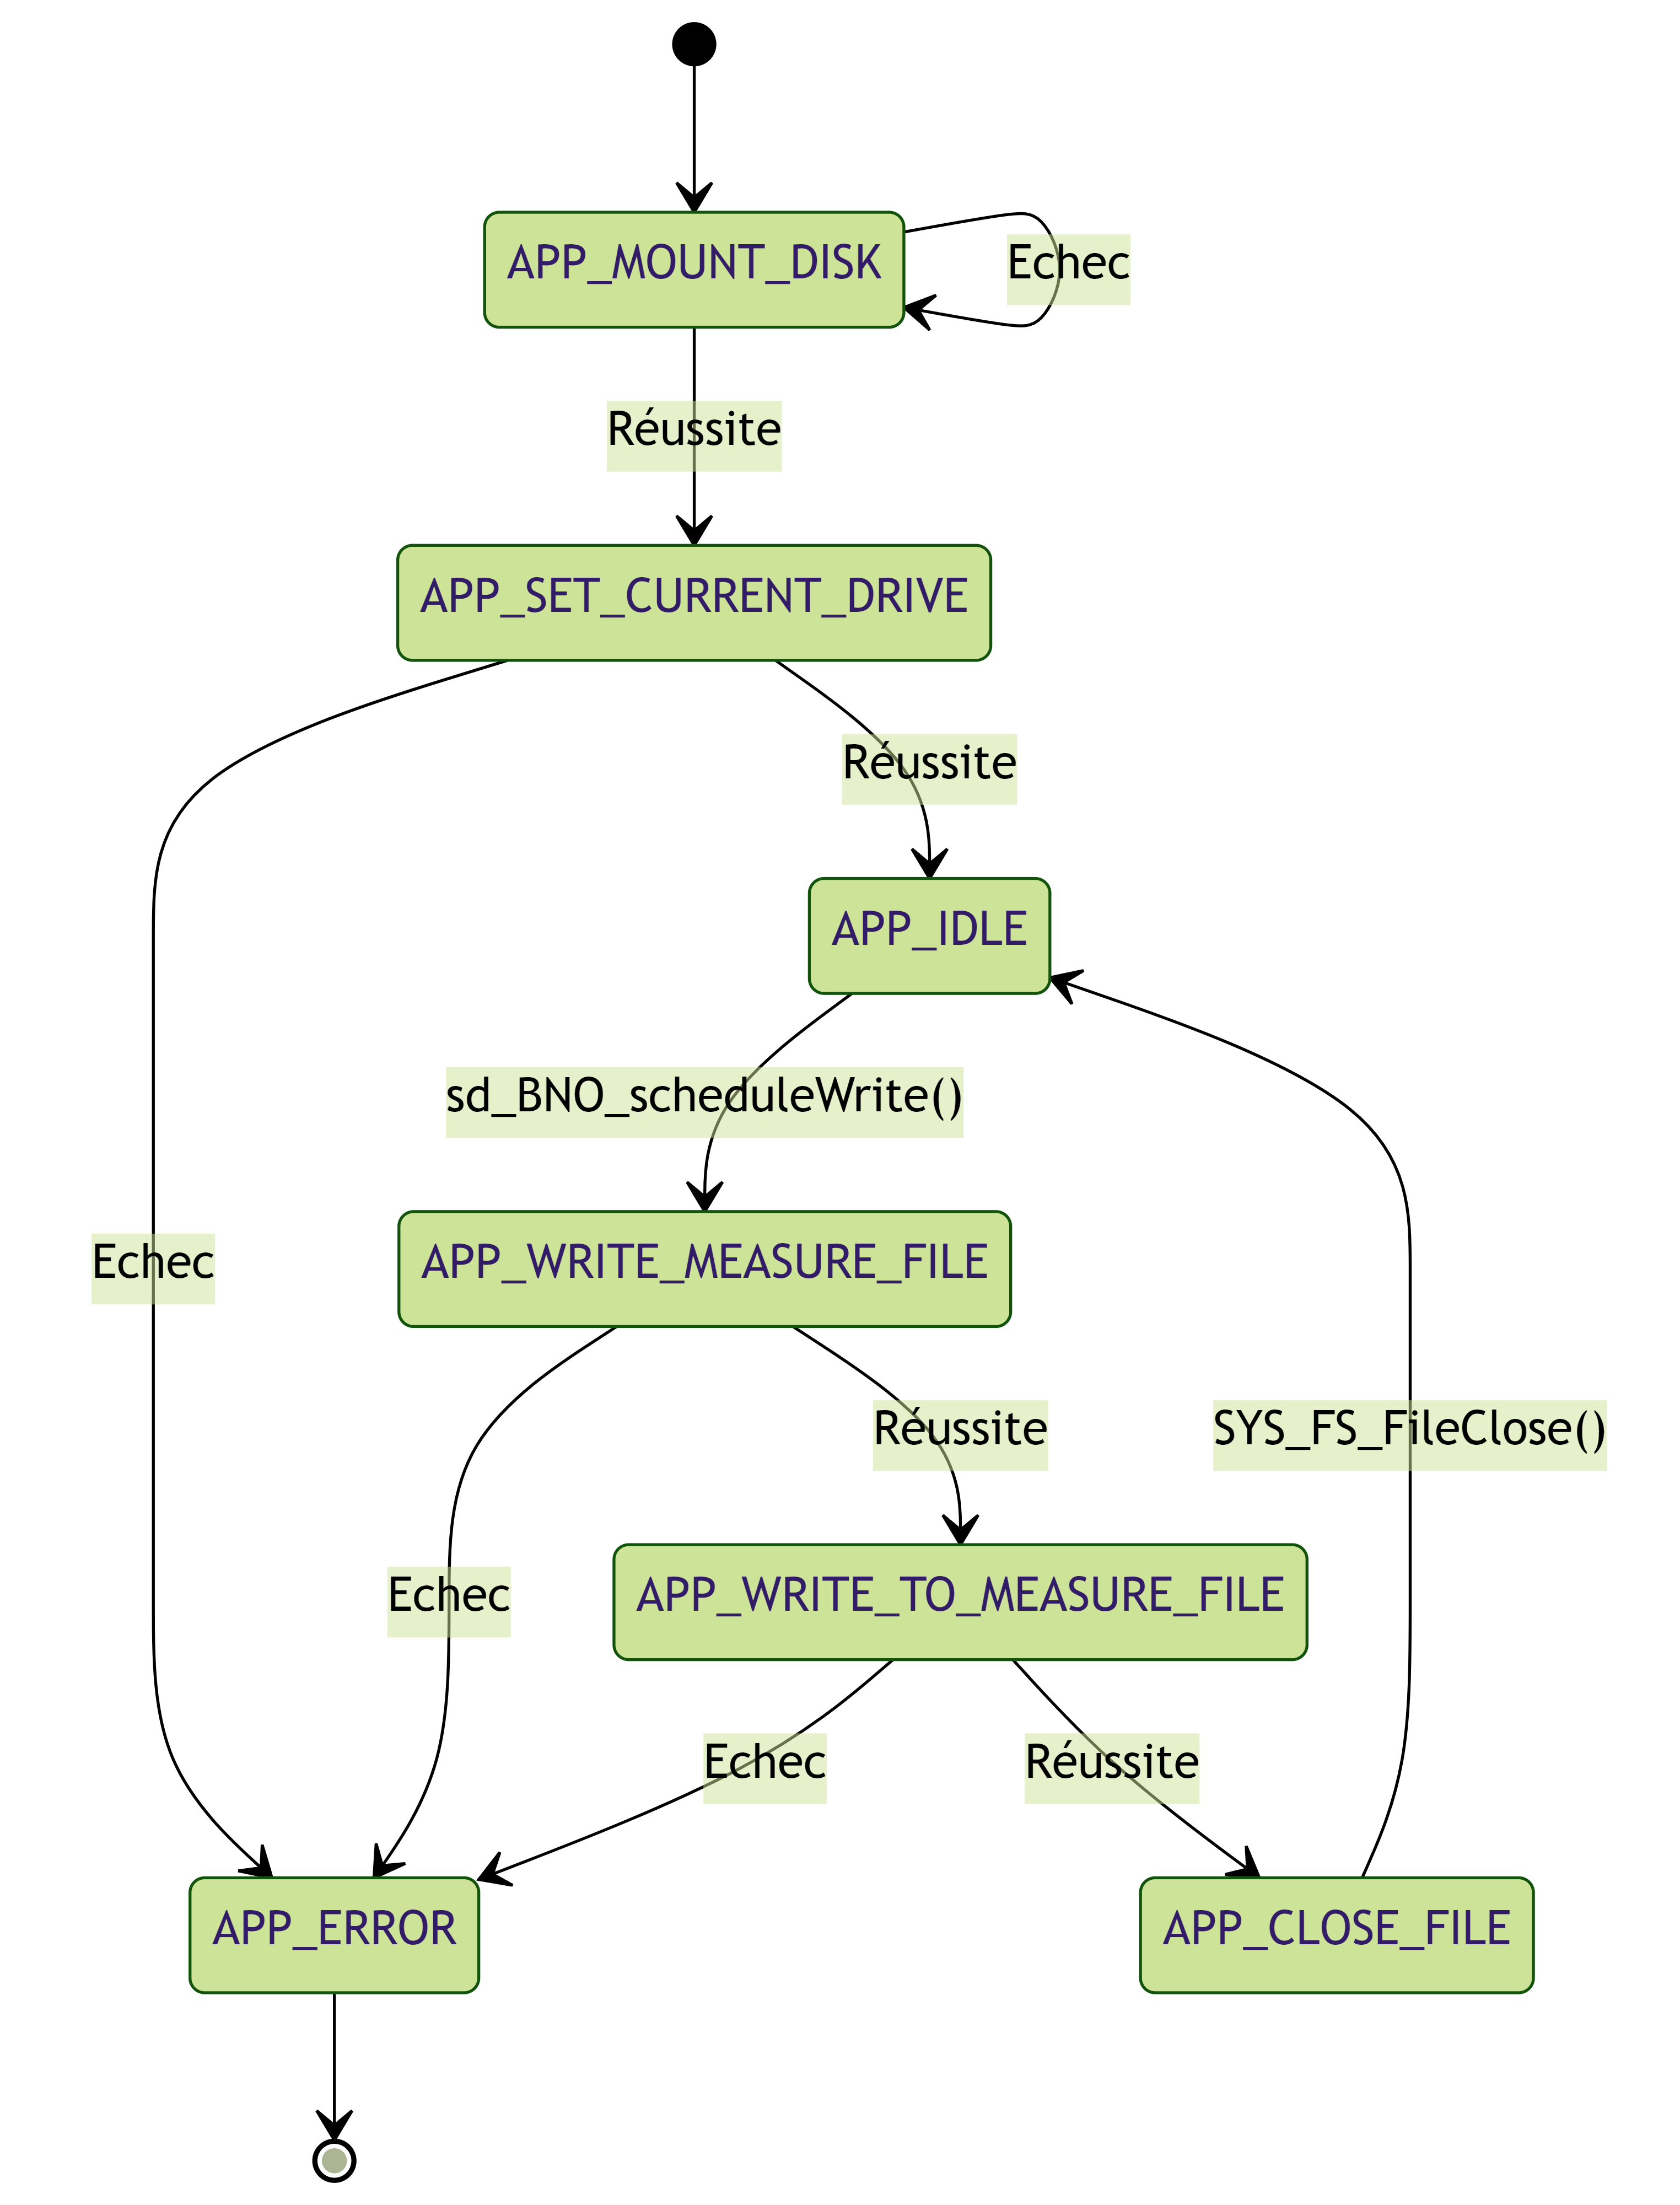
\includegraphics[width=0.6\linewidth]{Figures/Dev-SOFT/mermaid-diagram-2023-06-14-162436}
		\caption{Machine d'état de la carte SD}
		\label{fig:mermaid-diagram-2023-06-14-162436}
	\end{figure}

	\clearpage
	
	\paragraph{Planification d'une écriture}
	Afin de lancer une écriture d'un set de mesure sur la carte SD, il faut utiliser la fonction \textit{sd\_BNO\_scheduleWrite()} qui vas préparer le buffer d'écriture et modifier l'état de la carte SD : 
	\begin{lstlisting}[frame=single, language=C, caption={Lancement d'une écriture sur la carte SD}, captionpos=b, breaklines=true]
/* Write measures to sdCard */
sd_BNO_scheduleWrite(&bno055_local_data);
	\end{lstlisting}
	
	Les données sont écrite dans un fichier .CSV nommé "MESURES". La forme de la trame est la suivante :
	
	\begin{figure}[h]
		\centering
		
\includegraphics[width=1\textwidth]{Figures/Dev-SOFT/Trame}
		\caption{Format de la trame}
		\label{fig:trame}
	\end{figure}

	\begin{lstlisting}[frame=single, language=C, caption={Ecriture du buffer}, captionpos=b, breaklines=true]
"%d;%d0;%f;%.4f;%.4f;%.4f;%.4f;%.4f;%.4f;%.4f;%.4f;%.4f;%.4f;%.4f;%.4f;%.4f;%.4f;%.4f;%d;%d;%d;%d;"
	\end{lstlisting}
	
	\paragraph{Exemple trame CSV :} 
	0;372;1.025;-0.2500;0.3800;9.7900;-0.1250;0.1250;-0.0625;-44.8750;35.0625;-7.2500;0.0000;-0.0100;-0.2700;0.0000;-2.1875;-1.5000;16379;320;216;-1;

	
	\subsubsection{Application main}
	On peut visualiser la machine d'état de l'application principale sur la figure \ref{fig:stateapp}.
	\begin{figure}[h]
		\centering
		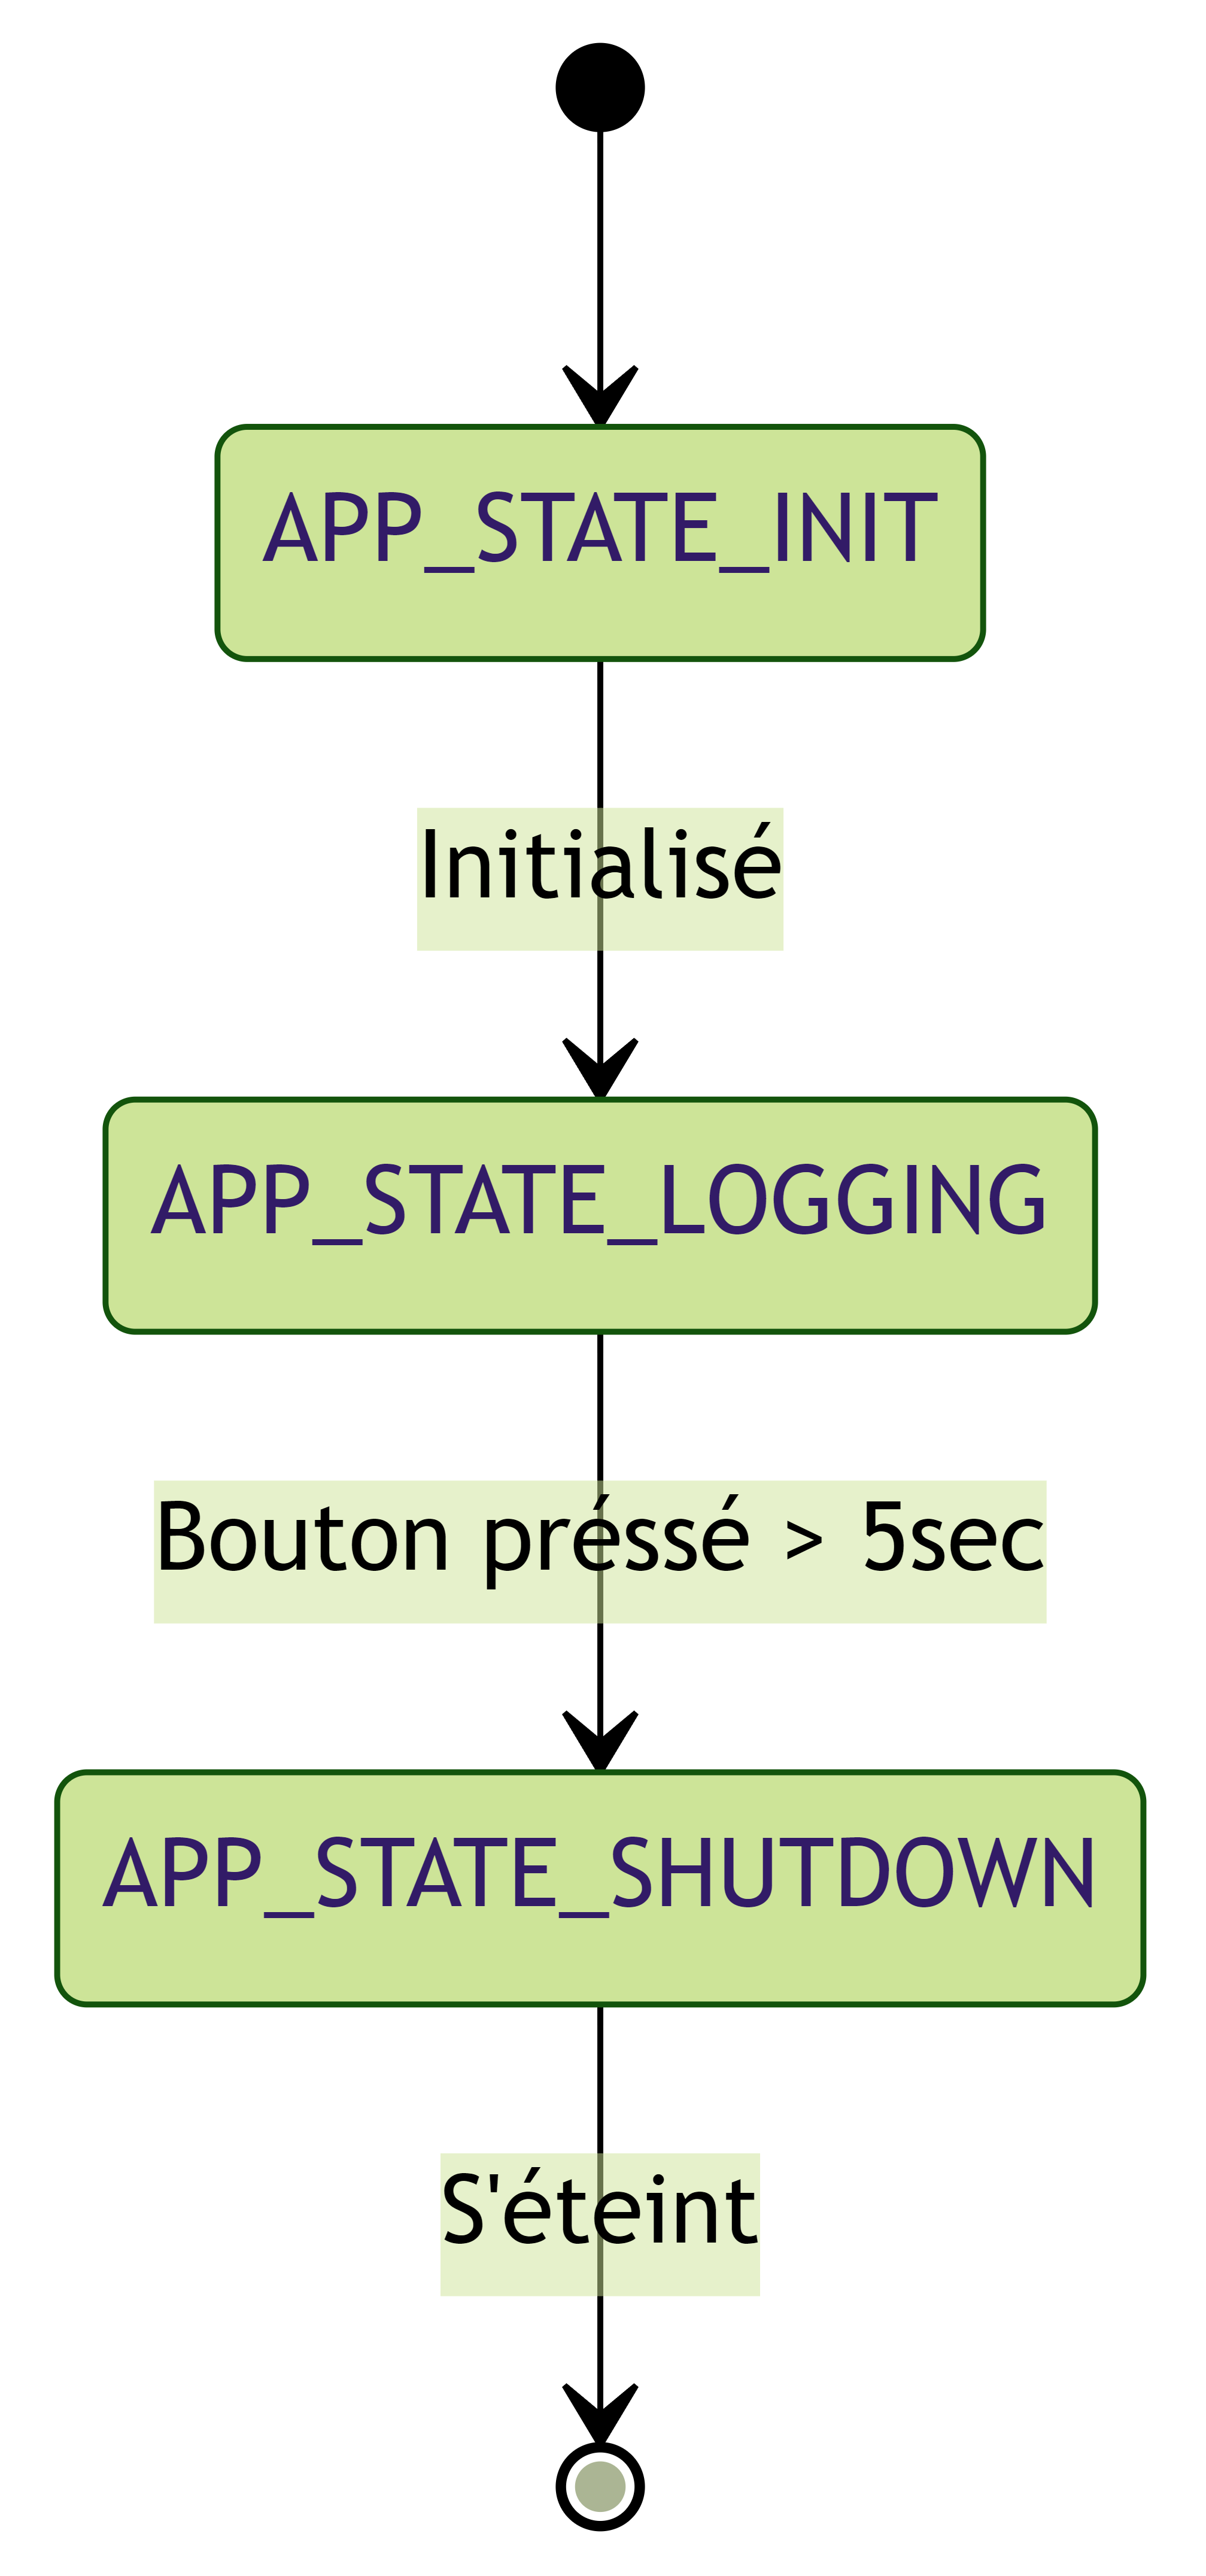
\includegraphics[width=0.28\linewidth]{Figures/Dev-SOFT/StateApp}
		\caption{Machine d'état application}
		\label{fig:stateapp}
	\end{figure}

	\clearpage
	
	\paragraph{Fonctionnement APP\_STATE\_LOGGING :} Une fois que l'application est en mode logging, le fonctionnement est décris sur la figure \ref{fig:appstatelogging} sous forme de flowchart.
	
	\begin{figure}[h]
		\centering
		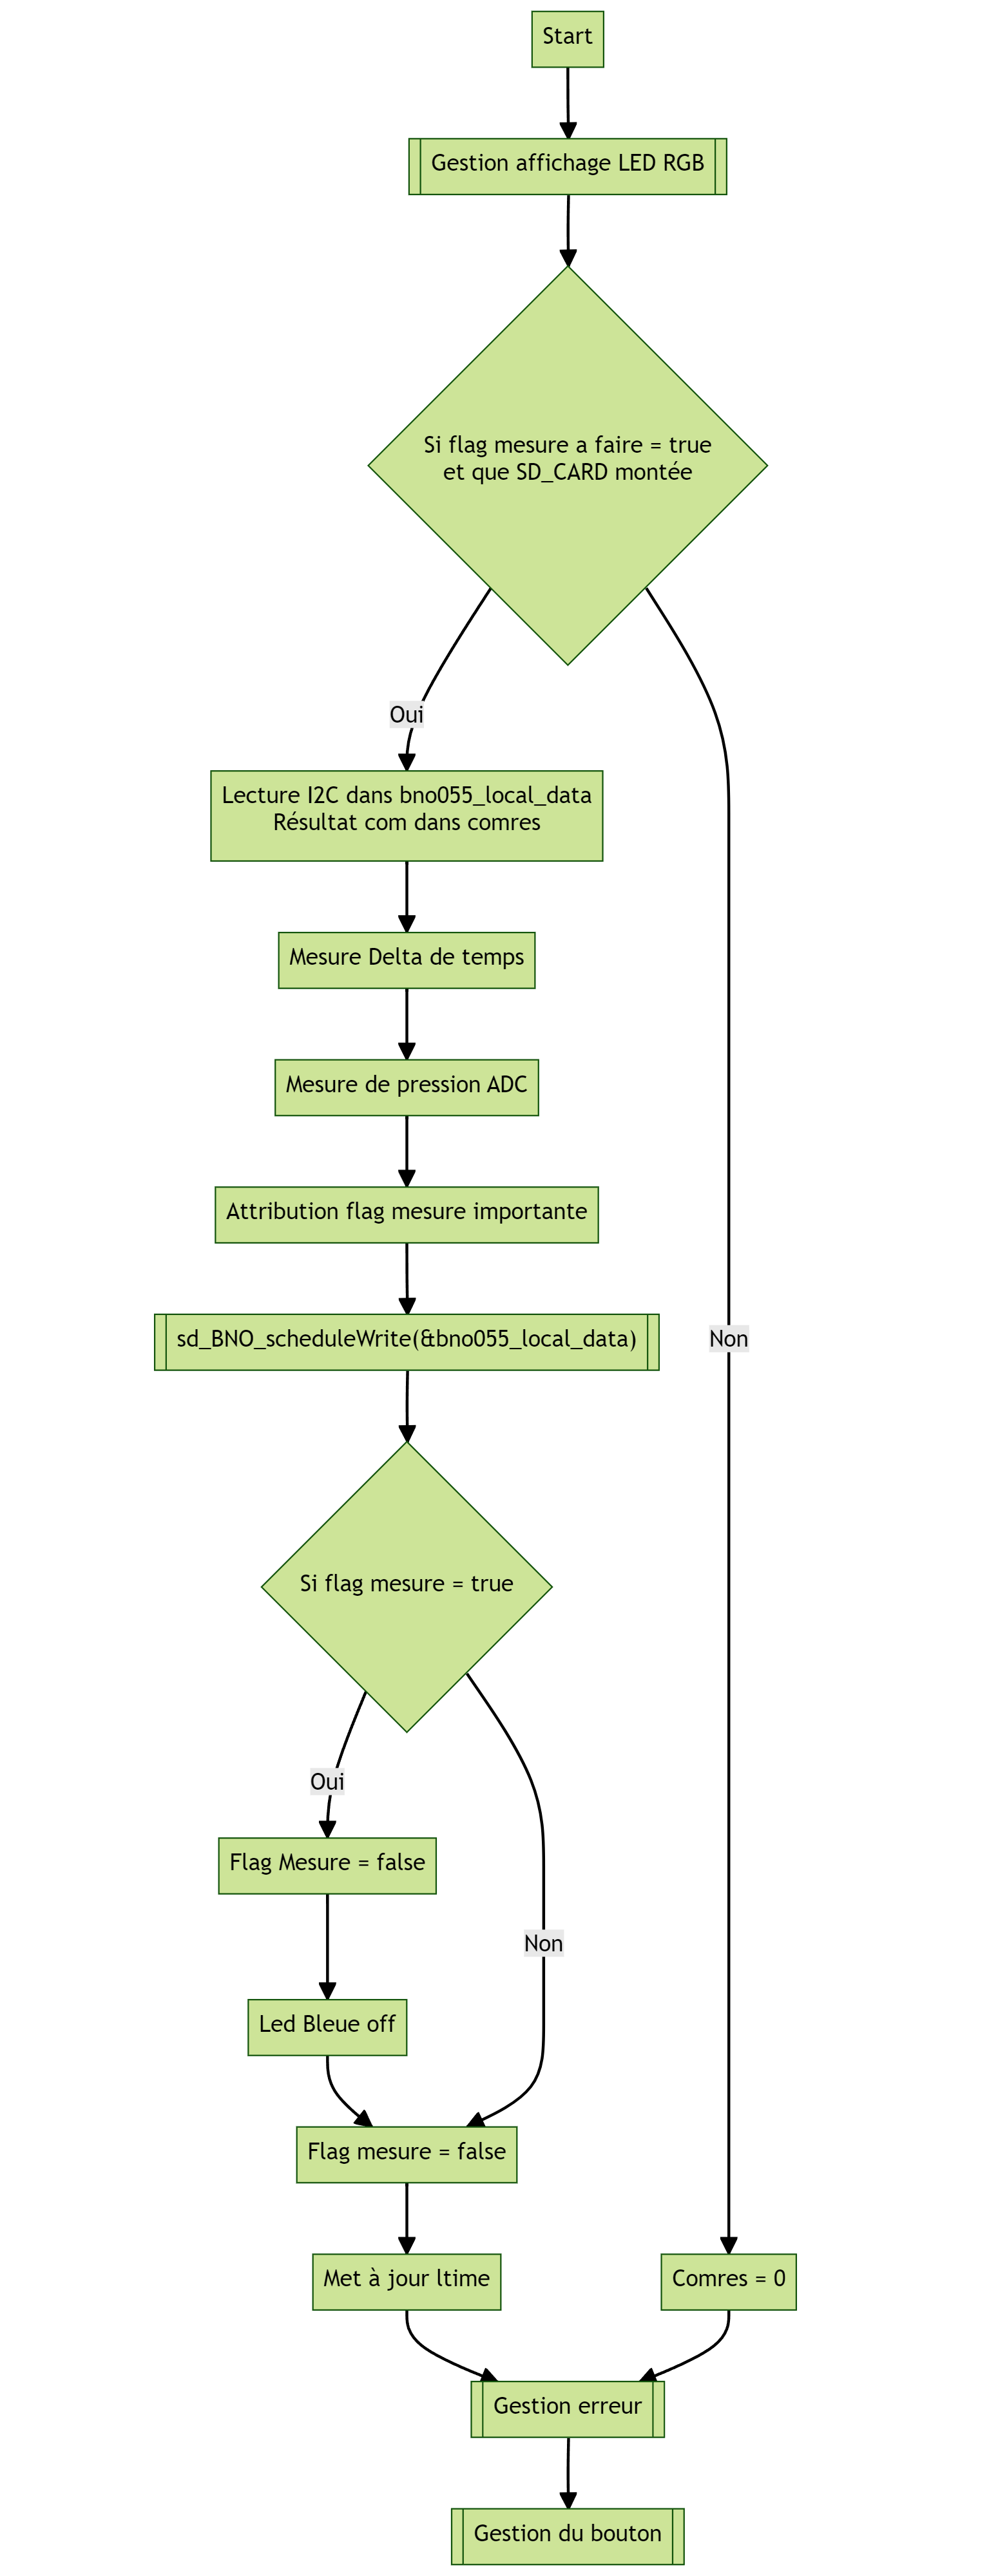
\includegraphics[width=0.446\linewidth]{Figures/Dev-SOFT/app_state_logging}
		\caption{Fowchart state logging}
		\label{fig:appstatelogging}
	\end{figure}

	\clearpage
	

}


% ---------- MESURE PREUVE DE CONCEPT ----------------------------- 
% !TeX spellcheck = fr_FR
\section{Validation du design}
Lors de cette section, sera décrite la procédure de vérification des caractéristiques du projet ainsi que sa validation.
\subsection{Liste de matériel} \label{ssec:ListeMateriel}
{
	\begin{enumerate}
		\item Oscilloscope Tektronix RTB2004 ES.SLO2.05.01.16 \label{enum:oscillo}
		\item Analyseur logique USB, 8 canaux, 24 MHz \label{enum:logicAnalyzer}
		\item USB vers TTL HW-597 \label{enum:USB-TTL}
		\item Carte Localisation-Sous-Marine V0.0 \label{enum:PCBL}
	\end{enumerate}
}

\subsection{Contrôle des alimentations}
{
	En premier lieu, une vérification des tensions d'alimentation permet de valider un aspect critique et fondamental de la carte.
	\subsubsection{Méthodologie}
	\paragraph{Mesure du 3.3V :} Alimentation de la carte par une connexion brève entre les pins du connecteur du bouton \textbf{P15}. Mesure sur le testpoint \textit{V\_regOUT5}, voir figure \ref{fig:sch3}.
	\begin{figure}[h]
		\centering
		\fbox{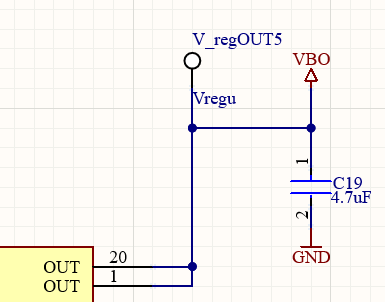
\includegraphics[width=0.3\linewidth]{Figures/DEV_MEAS/Sch3.3V}}
		\caption{Testpoint mesure 3.3V}
		\label{fig:sch3}
	\end{figure}
	
	\paragraph{Mesure du 5V :} Pour mesurer le 5V, il faut ponter par une résistance de $0\Omega$ la résistance R50, ainsi que activer la Pin RC5 / EN\_5V. Ensuite, la mesure a été prise sur le connecteur P16, pin-3, avec l'oscilloscope (Numéro \ref{enum:oscillo} de la liste de matériel \ref{ssec:ListeMateriel}) :
	\begin{figure}[h]
		\centering
		\fbox{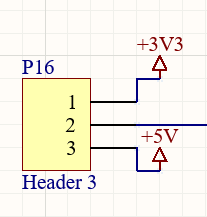
\includegraphics[width=0.2\linewidth]{Figures/DEV_MEAS/Sch5V}}
		\caption{Schéma de mesure 5V}
		\label{fig:sch5v}
	\end{figure}
	
	\clearpage
	
	\subsubsection{Mesures}
	
	\begin{figure}
		\begin{subfigure}{.5\textwidth}
			\centering
			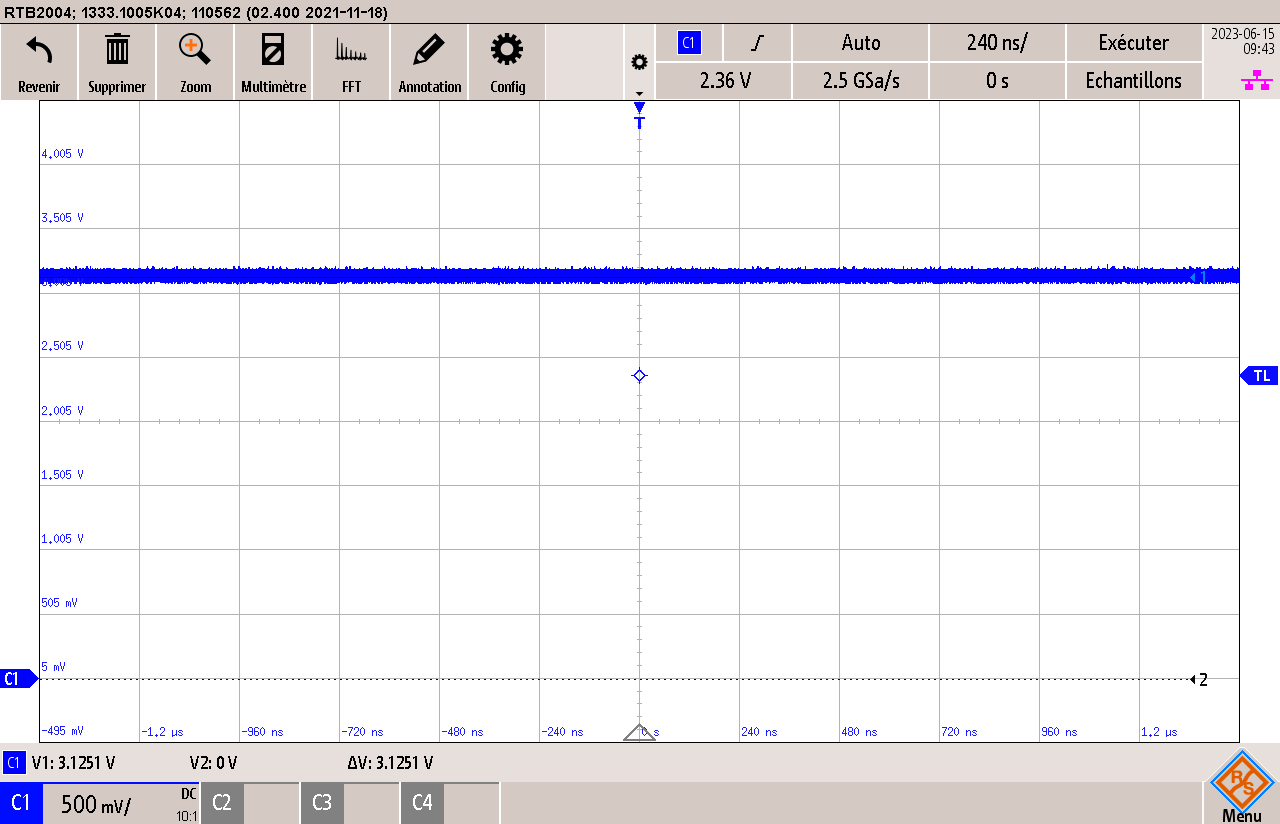
\includegraphics[width=\textwidth]{Mesures/Tension3.3V}
			\caption{Mesure 3.3V}
			\label{fig:Mes3.3V}
		\end{subfigure}
		\begin{subfigure}{.5\textwidth}
			\centering
			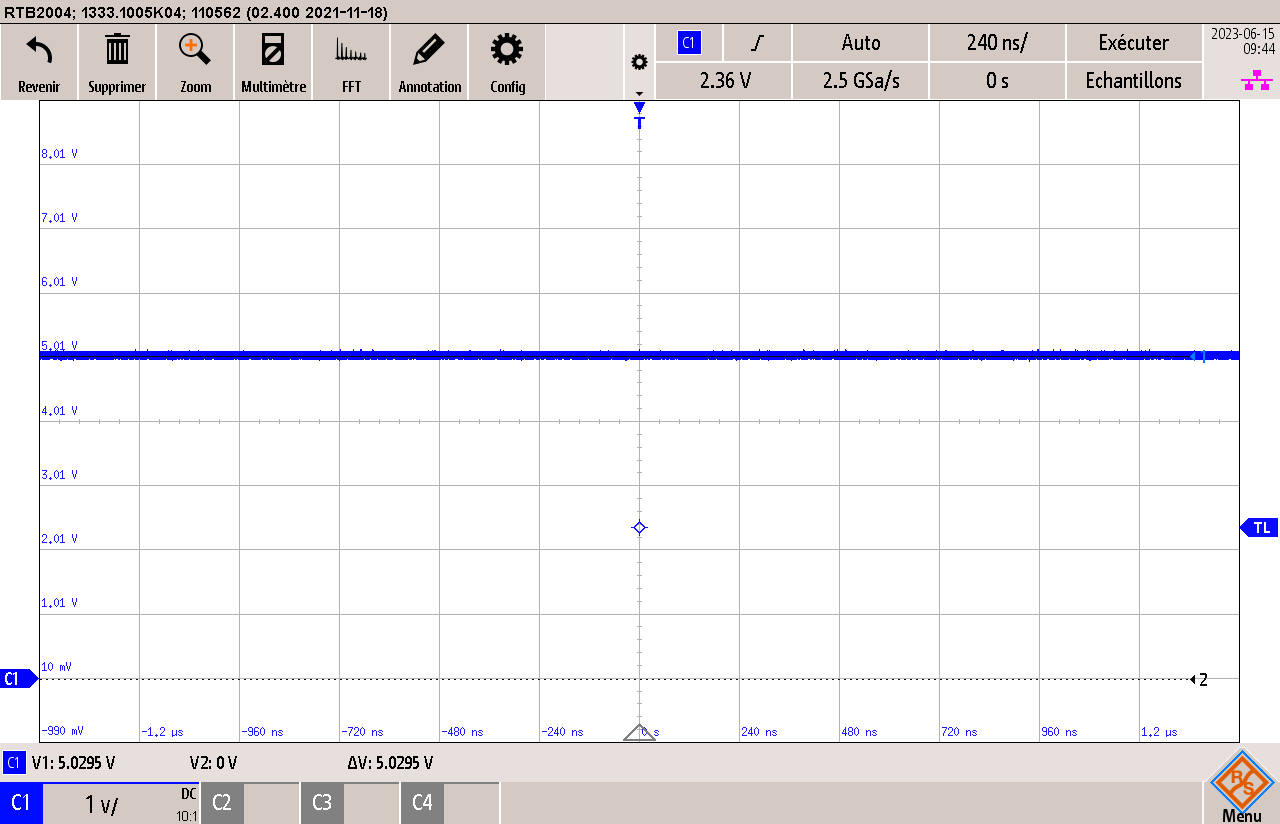
\includegraphics[width=\textwidth]{Mesures/Tension5V}
			\caption{Mesure 5V}
			\label{fig:Mes5V}
		\end{subfigure}
		\caption{Mesures des tensions d'alimentation}
		\label{fig:Mesure3.3et5V}
	\end{figure}
	
	\paragraph{Analyse :} Nous pouvons observer les valeurs respectives des tensions sur les figures \ref{fig:Mes3.3V} et \ref{fig:Mes5V}. La tension d'alimentation du microcontrôleur est mesurée à \textit{3.125V}, ce qui peut être expliqué par une chute de tension aux bornes de la batterie LI-ION qui nécessite donc d'être chargée. La tension 3.3V oscille légèrement, ce qui peut s'expliquer par le fait qu'il s'agit de l'alimentation principale de la carte avec le plus de consommateurs. Mais également par le fait que des signaux rapides sont générés par le microcontrôleur et ses différents périphériques.
	
	La tension d'alimentation du capteur de pression, dont la tension dimensionnée est de 5V, est quant à elle mesurée à \textit{5.0295V}, ce qui signifie une bonne précision de la part du circuit de boost. On peut également voir que la tension n'oscille pas et ne va donc pas perturber le capteur de pression.
	
	Nous pouvons donc confirmer le fonctionnement des blocs d'alimentation du projet.
}

\subsection{Communication UART}
{
	Comme décrit lors de la sous-section \ref{ssec:Usart}, une communication série est implémentée dans le projet. Cette communication n'est pas critique pour le projet, mais il est important de vérifier son fonctionnement pour d'éventuelles versions ultérieures.
	\subsubsection{Méthodologie}
	Pour la mesure, l'analyseur logique (Numéro \ref{enum:logicAnalyzer} de la liste de matériel \ref{ssec:ListeMateriel}) a été utilisé. Les trames U1TX et U1RX ont été mesurées sur le connecteur P4 :
	
	\begin{figure}[h]
		\centering
		\fbox{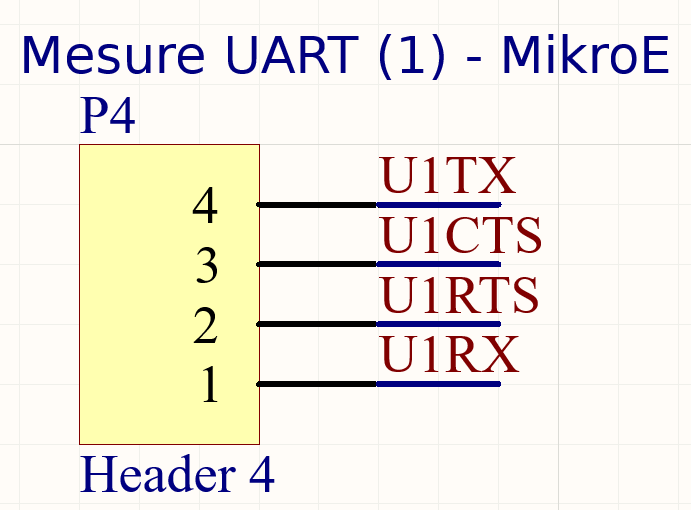
\includegraphics[width=0.2\linewidth]{Figures/DEV_MEAS/SchUart1}}
		\caption{Schéma de mesure UART1}
		\label{fig:schuart1}
	\end{figure}
	\clearpage	
	\subsubsection{Mesures}
	
	\begin{figure}[h]
		\centering
		\fbox{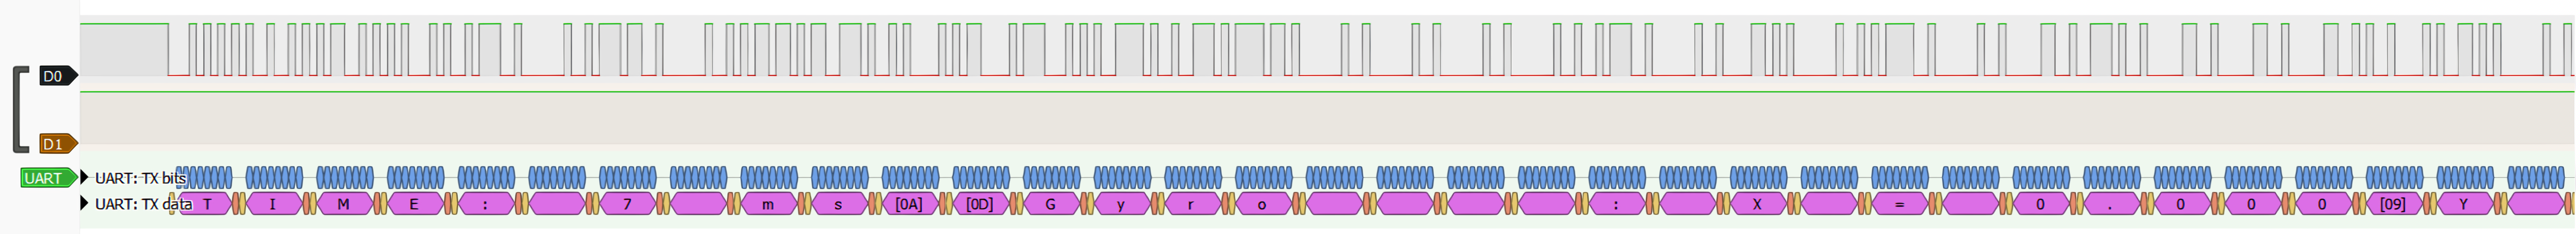
\includegraphics[width=1\linewidth]{Mesures/MesureTrameUart_Upscaled}}
		\caption{Mesures trames UART}
		\label{fig:mesuretrameuart}
	\end{figure}
	Nous pouvons lire des caractères ASCII sur la trame de la figure \ref{fig:mesuretrameuart}, qui reflètent le message envoyé contenant les mesures. 
	
	En connectant le module USB-TO-TTL (Numéro \ref{enum:USB-TTL} de la liste de matériel \ref{ssec:ListeMateriel}) aux broches Tx et Rx de la figure \ref{fig:mesuretrameuart}, puis en ouvrant une communication série via PuTTY à une baudrate de $115200$, nous obtenons la communication de la figure \ref{fig:puttytrames} dans la console :
	
	\begin{figure}[h]
		\centering
		\fbox{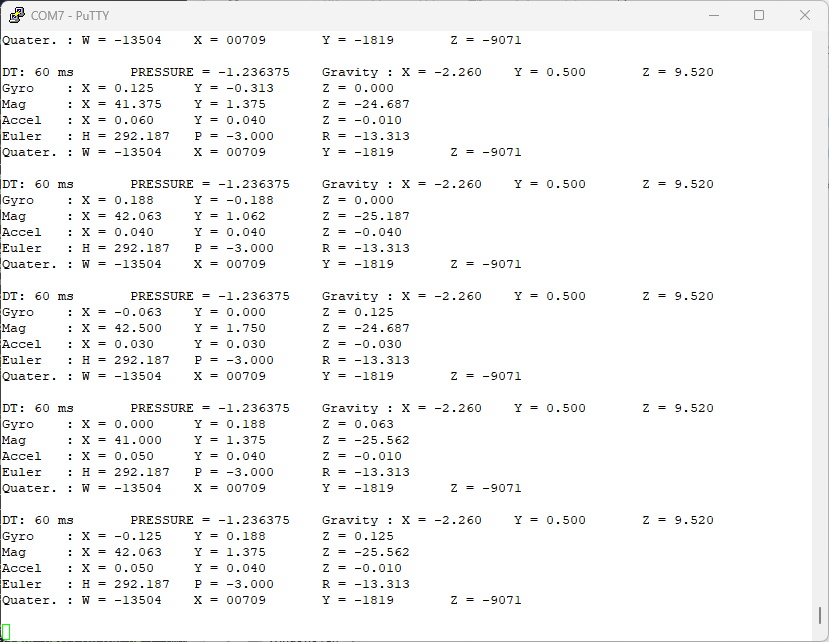
\includegraphics[width=0.65\linewidth]{Mesures/Putty_Trames}}
		\caption{Réception UART sur PuTTY}
		\label{fig:puttytrames}
	\end{figure}
	Analyse de la réception : Sur la figure \ref{fig:puttytrames}, on peut visualiser les données de la centrale inertielle, le temps écoulé entre chaque mesure, ainsi que les données du capteur de pression. Nous pouvons observer qu'entre chaque mesure, il s'écoule un laps de temps de $60 ms$, ce qui est plus rapide que les spécifications demandées par le cahier des charges. La mesure du capteur de pression à $-1.236$ bar n'est pas cohérente, car le capteur de pression n'était pas connecté au moment des mesures. Nous pouvons également constater que les mesures de la centrale inertielle sont cohérentes selon les données typiques d'une centrale inertielle\footnote{Exemple de données de fusion d'une centrale inertielle \cite{rozbicka2021estimation}}.
	
	\clearpage
}

\subsection{Communication SPI, carte SD}
{
	Il reste maintenant un élément critique à valider : la communication SPI avec la carte SD. Cette communication permet le logging des valeurs de mesure et est donc un aspect essentiel du projet.
	\subsubsection{Méthodologie}
	Pour cette mesure j'ai mesuré les signaux (SCK, SDO1, SDI1, CS\_SD) du SPI avec l'analyseur logique (Numéro \ref{enum:logicAnalyzer} de la liste de matériel \ref{ssec:ListeMateriel}).
	
	\begin{figure}[h]
		\centering
		\fbox{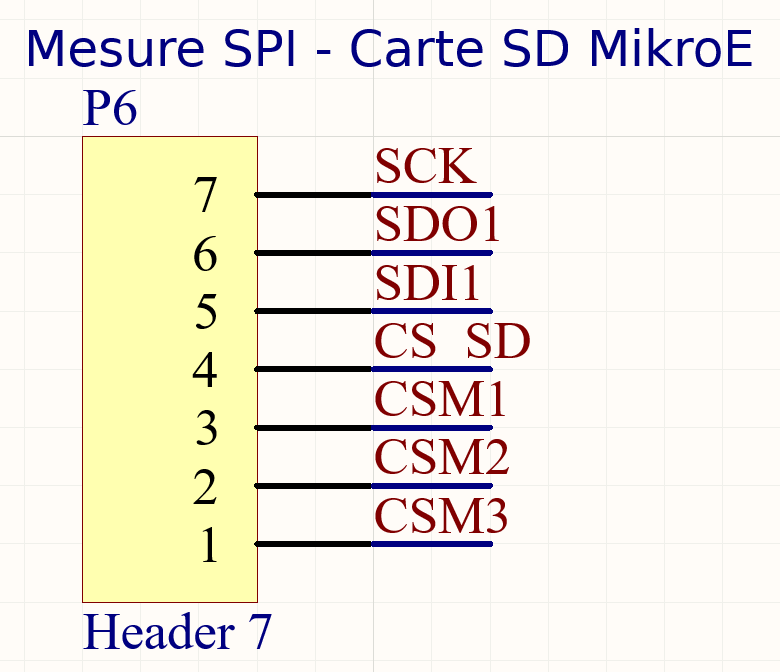
\includegraphics[width=0.35\linewidth]{Figures/DEV_MEAS/SchSpiSd}}
		\caption{Schéma de mesure carte SD}
		\label{fig:schspisd}
	\end{figure}
		
	\subsubsection{Mesures}
	\begin{figure}[h]
		\centering
		\includegraphics[width=1\linewidth]{Mesures/SPI_SD_CommEnsemble_Upscaled}
		\caption{Vue d'ensemble de la communication SPI}
		\label{fig:spisdcommensembleupscaled}
	\end{figure}
	Comme le montre la figure \ref{fig:spisdcommensembleupscaled}, on peut constater que les trames SPI utilisées pour la gestion de la FAT sont nombreuses. C'est pourquoi il est important d'avoir une fréquence élevée afin d'optimiser le temps des échanges de données.
	
	Nous allons maintenant mesurer le temps entre deux écritures sur la carte SD afin de vérifier le temps écoulé entre les mesures. et l'écriture.
	
	\clearpage
	
	\begin{figure}[h]
		\centering
		\includegraphics[width=1\linewidth]{Mesures/SPI_SD_TempreEntre2Comms_Upscaled}
		\caption{Temps entre deux écritures sur la carte SD}
		\label{fig:spisdtempreentre2commsupscaled}
	\end{figure}
	
	Nous pouvons observer sur la figure \ref{fig:spisdtempreentre2commsupscaled} que le temps mesuré entre une première écriture et le début de la suivante est de $89.804 ms$. Le temps disponible entre deux écritures est d'environ $\sim6ms$.
	Nous pouvons donc constater l'importance d'une vitesse élevée sur la communication SPI et sur le microcontrôleur.
	
	
	
	
	
}

\section{Caractéristiques du produit fini}

J'ai pu sans difficulté effectuer un logging de 5 heures et ai récolté 30 Mo de données dans le fichier CSV, ce qui correspond à environ 5 heures de logging.

% ---- Bibliographie ----
%\input{bibliography}

\clearpage

\section{Conclusion}
{
	\paragraph{Synthèse} Le présent rapport a décrit le développement et la validation d'un projet de localisation sous-marine. L'objectif principal du projet était de concevoir et de mettre en oeuvre un système capable de collecter et de stocker des données de déplacement, de temps et de pression lors de plongées. Après avoir réalisé les différentes étapes de développement, nous pouvons conclure que le projet a été mené à une version finie.
	
	\paragraph{Développement} Au cours de la phase de développement, plusieurs étapes clés ont été franchies. Tout d'abord, une analyse approfondie des besoins et des contraintes a été réalisée, ce qui a permis de définir les spécifications du système. Ensuite, un processus itératif de conception a été suivi, comprenant la sélection des composants appropriés, la création des schémas électroniques, et la fabrication du prototype.
	
	\paragraph{Design} L'évaluation du design du projet a été effectuée en suivant une méthodologie rigoureuse de vérification et de validation. Les principales caractéristiques du projet, telles que les tensions d'alimentation, la communication UART et la communication SPI avec la carte SD, ont été vérifiées avec succès. Les mesures effectuées ont montré que le système fonctionnait correctement et répondait aux spécifications requises.
	
	\paragraph{Test} Le projet a été testé avec succès lors d'un enregistrement de données de déplacement pendant une durée de 5 heures, ce qui a permis de collecter 30 MB de données. Ces résultats confirment que le système est capable de fonctionner de manière fiable et de fournir les fonctionnalités attendues.
	
	\paragraph{Apports} Ce projet a permis d'acquérir une expérience précieuse dans le domaine de la conception et du développement de systèmes électroniques. Il a également mis en évidence l'importance de l'organisation, de la structure et de la vérification étape par étape des éléments du design.
	
	\paragraph{Correctifs} Afin de simplifier la mise en place du système, des correctifs mentionnés dans le fichier MODIF (Section \ref{ssec:Modif}) permettrait de palier a certaines erreurs non-critiques de développements.
	
	\paragraph{Améliorations} Des améliorations et des développements futurs peuvent être envisagés, tels que l'ajout de fonctionnalités supplémentaires, l'optimisation de la communication, l'extension des capacités de stockage ainsi que la mise en place d'une communication USB directement par le FTDI en corrigeant le pinning de SCK. Ces évolutions permettraient d'explorer de nouvelles possibilités d'application de ce système de localisation sous-marine.
	
	\paragraph{Remerciements} Je tiens à remercier sincèrement M. Juan José Moreno, mon responsable de projet, Dr. Gaston Baudat pour avoir mandaté le projet et pour sa contribution algorithmique sur la localisation, et M. Fréderic Mueller pour son aide mécanique et pour la conception de la rallonge du module. Leur soutien et leur expertise ont été essentiels pour mener à bien ce projet. Je suis reconnaissant de leur précieuse collaboration et de leurs conseils tout au long du processus.
	
	
}


\newpage
\nocite{*}
\section{Bibliographie}
\bibliography{Biblio-Proj} 
\bibliographystyle{ieeetr}

% ANNEXES
\clearpage
\section{Annexes}

\begin{figure}[h]
	\centering
	\includegraphics[width=0.7\linewidth]{Figures/Annexes}
	\caption{Illustation annexes}
	\label{fig:annexes}
	\source{https://www.alamyimages.fr/photo-image-vecteur-icone-annexe-175637003.html}
\end{figure}

% Dossier Modif
\includepdf[scale=0.8,pages=1,pagecommand=\subsection{Fichier de modifs}\label{ssec:Modif}]{../../2221_LocalisationSousMarine-MOD-v1.pdf}

% Affiche
\includepdf[scale=0.8,pages=1,pagecommand=\subsection{Affiche du projet}\label{ssec:Affiche}]{../../2221_LocalisationSousMarine-AFFICHE.pdf}

% Résumé
\includepdf[scale=0.8,pages=1,pagecommand=\subsection{Résumé}\label{ssec:Resume}]{../../2221_LocalisationSousMarine-Résumé.pdf}

\subsection{Mode d'emploi}
\begin{enumerate}
	\item Insérer la carte SD format FAT.
	\item Allumer le système avec une impulsion sur le bouton.
	\subitem Si la LED clignote en vert,  le logging est en cours.
	\subitem Si la LED s'allume en rouge, il y a une erreur (Vérifier carte SD ou relancer système).
	\item Presser brièvement sur le bouton pour mettre la prochaine mesure en importance haute (1 dans CSV).
	\item Une fois le logging terminé, maintenir le bouton plus de 5 secondes pour éteindre le système.

\paragraph{Notes} Il est conseillé de bien éteindre le système par le bouton, pour ne pas mettre en danger l'intégrité de la carte SD. \vspace{+5mm}

	\item Retirer la carte SD.
	\item Insérer la carte SD sur un ordinateur avec un adaptateur.
	\item Récupérer le fichier \textit{MESURES.CSV}.
	\item Recommencer le cycle.
\end{enumerate}

% Schema
\includepdf[landscape=true, scale=0.9,pages=1,pagecommand=\subsection{Schéma électronique}\label{ssec:Schema}]{../../2221_Schematique.PDF}
\includepdf[landscape=true, scale=0.9,pages=2]{../../2221_Schematique.PDF}
\includepdf[landscape=true, scale=0.9,pages=3]{../../2221_Schematique.PDF}
\includepdf[landscape=true, scale=0.9,pages=4]{../../2221_Schematique.PDF}
\includepdf[landscape=true, scale=0.9,pages=5]{../../2221_Schematique.PDF}

% BOM
\includepdf[scale=0.8,pages=1,pagecommand=\subsection{Bill of materials}\label{ssec:BomAnnexe}]{../../bom/Bill of Materials.pdf}
\includepdf[scale=0.8,pages=2]{../../bom/Bill of Materials.pdf}

% Implémentation
\includepdf[scale=0.8,pages=1,pagecommand=\subsection{Implémentation}\label{ssec:Implementation}]{../../2221_Implémentation.PDF}
\includepdf[scale=0.8,pages=2]{../../2221_Implémentation.PDF}

\subsection{Code}

\begin{figure}[h]
	\centering
	\includegraphics[width=0.5\linewidth]{Figures/Illustration_code}
	\caption{Illustration code}
	\label{fig:illustrationcode}
	\source{https://www.vecteezy.com/vector-art/21464998-screen-coding-vector-illustration-on-a-background-premium-quality-symbols-vector-icons-for-concept-and-graphic-design}
\end{figure}


% Code
\includepdf[pages=-]{../../listing/LISTING.pdf}

% Journal de travail
\includepdf[scale=0.9,pages=1,pagecommand=\subsection{Journal de travail}\label{ssec:Journal}]{../../journal/Journal.pdf}

\includepdf[scale=0.9,pages=1,pagecommand=\subsection{Historique du Git}\label{ssec:GitHistory}]{../../journal/Git-History.pdf}
\includepdf[scale=0.9,pages=2]{../../journal/Git-History.pdf}
\includepdf[scale=0.9,pages=3]{../../journal/Git-History.pdf}
\includepdf[scale=0.9,pages=4]{../../journal/Git-History.pdf}
\includepdf[scale=0.9,pages=5]{../../journal/Git-History.pdf}


\end{document}
